\documentclass[]{book}
\usepackage{lmodern}
\usepackage{amssymb,amsmath}
\usepackage{ifxetex,ifluatex}
\usepackage{fixltx2e} % provides \textsubscript
\ifnum 0\ifxetex 1\fi\ifluatex 1\fi=0 % if pdftex
  \usepackage[T1]{fontenc}
  \usepackage[utf8]{inputenc}
\else % if luatex or xelatex
  \ifxetex
    \usepackage{mathspec}
  \else
    \usepackage{fontspec}
  \fi
  \defaultfontfeatures{Ligatures=TeX,Scale=MatchLowercase}
\fi
% use upquote if available, for straight quotes in verbatim environments
\IfFileExists{upquote.sty}{\usepackage{upquote}}{}
% use microtype if available
\IfFileExists{microtype.sty}{%
\usepackage{microtype}
\UseMicrotypeSet[protrusion]{basicmath} % disable protrusion for tt fonts
}{}
\usepackage[margin=1in]{geometry}
\usepackage{hyperref}
\hypersetup{unicode=true,
            pdftitle={R语言模型部署实战},
            pdfauthor={徐静},
            pdfborder={0 0 0},
            breaklinks=true}
\urlstyle{same}  % don't use monospace font for urls
\usepackage{natbib}
\bibliographystyle{apalike}
\usepackage{color}
\usepackage{fancyvrb}
\newcommand{\VerbBar}{|}
\newcommand{\VERB}{\Verb[commandchars=\\\{\}]}
\DefineVerbatimEnvironment{Highlighting}{Verbatim}{commandchars=\\\{\}}
% Add ',fontsize=\small' for more characters per line
\usepackage{framed}
\definecolor{shadecolor}{RGB}{248,248,248}
\newenvironment{Shaded}{\begin{snugshade}}{\end{snugshade}}
\newcommand{\KeywordTok}[1]{\textcolor[rgb]{0.13,0.29,0.53}{\textbf{#1}}}
\newcommand{\DataTypeTok}[1]{\textcolor[rgb]{0.13,0.29,0.53}{#1}}
\newcommand{\DecValTok}[1]{\textcolor[rgb]{0.00,0.00,0.81}{#1}}
\newcommand{\BaseNTok}[1]{\textcolor[rgb]{0.00,0.00,0.81}{#1}}
\newcommand{\FloatTok}[1]{\textcolor[rgb]{0.00,0.00,0.81}{#1}}
\newcommand{\ConstantTok}[1]{\textcolor[rgb]{0.00,0.00,0.00}{#1}}
\newcommand{\CharTok}[1]{\textcolor[rgb]{0.31,0.60,0.02}{#1}}
\newcommand{\SpecialCharTok}[1]{\textcolor[rgb]{0.00,0.00,0.00}{#1}}
\newcommand{\StringTok}[1]{\textcolor[rgb]{0.31,0.60,0.02}{#1}}
\newcommand{\VerbatimStringTok}[1]{\textcolor[rgb]{0.31,0.60,0.02}{#1}}
\newcommand{\SpecialStringTok}[1]{\textcolor[rgb]{0.31,0.60,0.02}{#1}}
\newcommand{\ImportTok}[1]{#1}
\newcommand{\CommentTok}[1]{\textcolor[rgb]{0.56,0.35,0.01}{\textit{#1}}}
\newcommand{\DocumentationTok}[1]{\textcolor[rgb]{0.56,0.35,0.01}{\textbf{\textit{#1}}}}
\newcommand{\AnnotationTok}[1]{\textcolor[rgb]{0.56,0.35,0.01}{\textbf{\textit{#1}}}}
\newcommand{\CommentVarTok}[1]{\textcolor[rgb]{0.56,0.35,0.01}{\textbf{\textit{#1}}}}
\newcommand{\OtherTok}[1]{\textcolor[rgb]{0.56,0.35,0.01}{#1}}
\newcommand{\FunctionTok}[1]{\textcolor[rgb]{0.00,0.00,0.00}{#1}}
\newcommand{\VariableTok}[1]{\textcolor[rgb]{0.00,0.00,0.00}{#1}}
\newcommand{\ControlFlowTok}[1]{\textcolor[rgb]{0.13,0.29,0.53}{\textbf{#1}}}
\newcommand{\OperatorTok}[1]{\textcolor[rgb]{0.81,0.36,0.00}{\textbf{#1}}}
\newcommand{\BuiltInTok}[1]{#1}
\newcommand{\ExtensionTok}[1]{#1}
\newcommand{\PreprocessorTok}[1]{\textcolor[rgb]{0.56,0.35,0.01}{\textit{#1}}}
\newcommand{\AttributeTok}[1]{\textcolor[rgb]{0.77,0.63,0.00}{#1}}
\newcommand{\RegionMarkerTok}[1]{#1}
\newcommand{\InformationTok}[1]{\textcolor[rgb]{0.56,0.35,0.01}{\textbf{\textit{#1}}}}
\newcommand{\WarningTok}[1]{\textcolor[rgb]{0.56,0.35,0.01}{\textbf{\textit{#1}}}}
\newcommand{\AlertTok}[1]{\textcolor[rgb]{0.94,0.16,0.16}{#1}}
\newcommand{\ErrorTok}[1]{\textcolor[rgb]{0.64,0.00,0.00}{\textbf{#1}}}
\newcommand{\NormalTok}[1]{#1}
\usepackage{longtable,booktabs}
\usepackage{graphicx,grffile}
\makeatletter
\def\maxwidth{\ifdim\Gin@nat@width>\linewidth\linewidth\else\Gin@nat@width\fi}
\def\maxheight{\ifdim\Gin@nat@height>\textheight\textheight\else\Gin@nat@height\fi}
\makeatother
% Scale images if necessary, so that they will not overflow the page
% margins by default, and it is still possible to overwrite the defaults
% using explicit options in \includegraphics[width, height, ...]{}
\setkeys{Gin}{width=\maxwidth,height=\maxheight,keepaspectratio}
\IfFileExists{parskip.sty}{%
\usepackage{parskip}
}{% else
\setlength{\parindent}{0pt}
\setlength{\parskip}{6pt plus 2pt minus 1pt}
}
\setlength{\emergencystretch}{3em}  % prevent overfull lines
\providecommand{\tightlist}{%
  \setlength{\itemsep}{0pt}\setlength{\parskip}{0pt}}
\setcounter{secnumdepth}{5}
% Redefines (sub)paragraphs to behave more like sections
\ifx\paragraph\undefined\else
\let\oldparagraph\paragraph
\renewcommand{\paragraph}[1]{\oldparagraph{#1}\mbox{}}
\fi
\ifx\subparagraph\undefined\else
\let\oldsubparagraph\subparagraph
\renewcommand{\subparagraph}[1]{\oldsubparagraph{#1}\mbox{}}
\fi

%%% Use protect on footnotes to avoid problems with footnotes in titles
\let\rmarkdownfootnote\footnote%
\def\footnote{\protect\rmarkdownfootnote}

%%% Change title format to be more compact
\usepackage{titling}

% Create subtitle command for use in maketitle
\newcommand{\subtitle}[1]{
  \posttitle{
    \begin{center}\large#1\end{center}
    }
}

\setlength{\droptitle}{-2em}

  \title{R语言模型部署实战}
    \pretitle{\vspace{\droptitle}\centering\huge}
  \posttitle{\par}
    \author{徐静}
    \preauthor{\centering\large\emph}
  \postauthor{\par}
      \predate{\centering\large\emph}
  \postdate{\par}
    \date{2018-12-31}

\usepackage{booktabs}
\usepackage{xeCJK}

\setCJKmainfont{宋体}

\setmainfont{Georgia}

\setromanfont{Georgia}

\setmonofont{Courier New}

\begin{document}
\maketitle

{
\setcounter{tocdepth}{1}
\tableofcontents
}
\chapter*{序言}
\addcontentsline{toc}{chapter}{序言}

我们的模型不能只停留在线下的分析报告中,训练好的R模型如何应用到生产环境?目前针对于R语言的模型生产环境应用的方式有很多,比如用其他语言去调用,Java,Python等语言均可方便的调用R脚本;生成PMML文件,目前R中主流的一些R模型均支持PMML比如xgboost,lightGBM等,其他语言不需要调用R脚本只需调用统一的PMML文件就可以;还有就是Web端的部署,比如可以做成REST
API供其他语言调用,或直接做成web应用供其他用户访问,本书主要针对于R语言模型的Web端的部署。过程中,我们会先后介绍httpuv,opencpu,plumber,
jug,fiery,Rserve,RestRserve,等一些和模型线上化部署相关的R包(当然shiny也可以,但他不是我们本书的重点),最后会介绍mailR和Rweixin两个R和邮件与微信通信的R包,用于线上化部署的监测。当然会有其他的线上化部署方式。

欢迎进入R模型线上化部署的海洋!

\chapter*{关于我}
\addcontentsline{toc}{chapter}{关于我}

\textbf{徐静:}

硕士研究生,
目前的研究兴趣主要包括:数理统计,统计机器学习,深度学习,网络爬虫,前端可视化,R语言和Python语言的超级粉丝,多个R包和Python模块的作者,现在正逐步向Java迁移。

Graduate students,the current research interests include: mathematical
statistics, statistical machine learning, deep learning, web crawler,
front-end visualization. He is a super fan of R and Python, and the
author of several R packages and Python modules, and now gradually
migrating to Java.

\chapter{httpuv}\label{httpuv}

在httpuv的官网中,有这么一段描述:

\begin{quote}
Allows R code to listen for and interact with HTTP and WebSocket
clients, so you can serve web traffic directly out of your R process.
Implementation is based on libuv and http-parser.
\end{quote}

\begin{quote}
This is a low-level library that provides little more than network I/O
and implementations of the HTTP and WebSocket protocols. For an easy way
to create web applications, try Shiny instead.
\end{quote}

我们可以通过httpuv搭建一个访问R模型的web API,但可能这不是最好的。

本部分我们首先介绍官方提供的一些方法,然后解析官方提供的演示Demo,从而达到熟练使用httpuv的目的。

\section{方法介绍}

下面我们解析一下httpuv官方提供的一些调用方法,并演示一些调用方法对应的实例

1.使用URI编码/解码以与Web浏览器相同的方式对字符串进行编码/解码。

\begin{Shaded}
\begin{Highlighting}[]
\KeywordTok{encodeURI}\NormalTok{(value)}
\KeywordTok{encodeURIComponent}\NormalTok{(value)}
\KeywordTok{decodeURI}\NormalTok{(value)}
\KeywordTok{decodeURIComponent}\NormalTok{(value)}
\end{Highlighting}
\end{Shaded}

参数列表

\begin{itemize}
\tightlist
\item
  value 用于编码和解码的字符向量,UTF-8字符编码
\end{itemize}

\begin{Shaded}
\begin{Highlighting}[]
\KeywordTok{library}\NormalTok{(httpuv)}
\NormalTok{value <-}\StringTok{ "https://baidu.com/中国;?/"}
\KeywordTok{encodeURI}\NormalTok{(value)}
\end{Highlighting}
\end{Shaded}

\begin{verbatim}
## [1] "https://baidu.com/%D6%D0%B9%FA;?/"
\end{verbatim}

\begin{Shaded}
\begin{Highlighting}[]
\KeywordTok{encodeURIComponent}\NormalTok{(value)}
\end{Highlighting}
\end{Shaded}

\begin{verbatim}
## [1] "https%3A%2F%2Fbaidu.com%2F%D6%D0%B9%FA%3B%3F%2F"
\end{verbatim}

\begin{Shaded}
\begin{Highlighting}[]
\KeywordTok{decodeURI}\NormalTok{(value)}
\end{Highlighting}
\end{Shaded}

\begin{verbatim}
## [1] "https://baidu.com/中国;?/"
\end{verbatim}

\begin{Shaded}
\begin{Highlighting}[]
\KeywordTok{decodeURIComponent}\NormalTok{(value)}
\end{Highlighting}
\end{Shaded}

\begin{verbatim}
## [1] "https://baidu.com/中国;?/"
\end{verbatim}

注意: encodeURI 与 encodeURIComponent是不一样的因为前者不对特殊字符:
;,/?:@\&=+\$等进行encode

2.中断httpuv运行的环路

\begin{Shaded}
\begin{Highlighting}[]
\KeywordTok{interrupt}\NormalTok{()}
\end{Highlighting}
\end{Shaded}

\begin{enumerate}
\def\labelenumi{\arabic{enumi}.}
\setcounter{enumi}{2}
\tightlist
\item
  检查ip地址的类型是ipv4还是ipv6
\end{enumerate}

\begin{Shaded}
\begin{Highlighting}[]
\KeywordTok{ipFamily}\NormalTok{(ip)}
\end{Highlighting}
\end{Shaded}

参数列表

\begin{itemize}
\item
  ip 一个代表IP地址的字符串
\item
  返回值的意义:如果是IPv4返回4,如果是IPv6返回6,如果不是IP地址返回-1
\end{itemize}

\begin{Shaded}
\begin{Highlighting}[]
\KeywordTok{ipFamily}\NormalTok{(}\StringTok{"127.0.0.1"}\NormalTok{) }\CommentTok{# 4}
\end{Highlighting}
\end{Shaded}

\begin{verbatim}
## [1] 4
\end{verbatim}

\begin{Shaded}
\begin{Highlighting}[]
\KeywordTok{ipFamily}\NormalTok{(}\StringTok{"500.0.0.500"}\NormalTok{) }\CommentTok{# -1}
\end{Highlighting}
\end{Shaded}

\begin{verbatim}
## [1] -1
\end{verbatim}

\begin{Shaded}
\begin{Highlighting}[]
\KeywordTok{ipFamily}\NormalTok{(}\StringTok{"500.0.0.500"}\NormalTok{) }\CommentTok{# -1}
\end{Highlighting}
\end{Shaded}

\begin{verbatim}
## [1] -1
\end{verbatim}

\begin{Shaded}
\begin{Highlighting}[]
\KeywordTok{ipFamily}\NormalTok{(}\StringTok{"::"}\NormalTok{) }\CommentTok{# 6}
\end{Highlighting}
\end{Shaded}

\begin{verbatim}
## [1] 6
\end{verbatim}

\begin{Shaded}
\begin{Highlighting}[]
\KeywordTok{ipFamily}\NormalTok{(}\StringTok{"::1"}\NormalTok{) }\CommentTok{# 6}
\end{Highlighting}
\end{Shaded}

\begin{verbatim}
## [1] 6
\end{verbatim}

\begin{Shaded}
\begin{Highlighting}[]
\KeywordTok{ipFamily}\NormalTok{(}\StringTok{"fe80::1ff:fe23:4567:890a"}\NormalTok{) }\CommentTok{# 6}
\end{Highlighting}
\end{Shaded}

\begin{verbatim}
## [1] 6
\end{verbatim}

3.将原始向量转换为BASE64编码字符串

\begin{Shaded}
\begin{Highlighting}[]
\KeywordTok{rawToBase64}\NormalTok{(x)}
\end{Highlighting}
\end{Shaded}

参数列表

\begin{itemize}
\tightlist
\item
  x 原始向量
\end{itemize}

\begin{Shaded}
\begin{Highlighting}[]
\KeywordTok{set.seed}\NormalTok{(}\DecValTok{100}\NormalTok{)}
\NormalTok{result <-}\StringTok{ }\KeywordTok{rawToBase64}\NormalTok{(}\KeywordTok{as.raw}\NormalTok{(}\KeywordTok{runif}\NormalTok{(}\DecValTok{19}\NormalTok{, }\DataTypeTok{min=}\DecValTok{0}\NormalTok{, }\DataTypeTok{max=}\DecValTok{256}\NormalTok{)))}
\CommentTok{#stopifnot(identical(result, "TkGNDnd7z16LK5/hR2bDqzRbXA=="))}
\NormalTok{result}
\end{Highlighting}
\end{Shaded}

\begin{verbatim}
## [1] "TkGNDnd7z16LK5/hR2bDqzRbXA=="
\end{verbatim}

4.运行一个server

\begin{Shaded}
\begin{Highlighting}[]
\KeywordTok{runServer}\NormalTok{(host, port, app, }\DataTypeTok{interruptIntervalMs =} \OtherTok{NULL}\NormalTok{)}
\end{Highlighting}
\end{Shaded}

参数列表

\begin{itemize}
\item
  host IPv4地址, 或是``0.0.0.0''监听所有的IP
\item
  port 端口号
\item
  app 一个定义应用的函数集合
\item
  interruptIntervalMs 该参数不提倡使用,1.3.5版本后废除
\end{itemize}

\begin{Shaded}
\begin{Highlighting}[]
\NormalTok{app <-}\StringTok{ }\KeywordTok{list}\NormalTok{(}\DataTypeTok{call =} \ControlFlowTok{function}\NormalTok{(req)\{}
  \KeywordTok{list}\NormalTok{(}\DataTypeTok{status=}\NormalTok{200L,}
       \DataTypeTok{headers =} \KeywordTok{list}\NormalTok{(}
         \StringTok{'Content-Type'}\NormalTok{ =}\StringTok{ 'text/html'}
\NormalTok{       ),}
       \DataTypeTok{body =} \StringTok{"HelloWorld!"}\NormalTok{)}
\NormalTok{\})}

\KeywordTok{runServer}\NormalTok{(}\StringTok{"0.0.0.0"}\NormalTok{, }\DecValTok{5000}\NormalTok{,app)}
\end{Highlighting}
\end{Shaded}

5.过程请求

处理HTTP请求和WebSocket消息。 如果R的调用堆栈上没有任何东西,如果R是
在命令提示符下闲置,不必调用此函数,因为请求将
自动处理。但是,如果R正在执行代码,则请求将不被处理。
要么调用栈是空的,要么调用这个函数(或者,调用run\_now())。

\begin{Shaded}
\begin{Highlighting}[]
\KeywordTok{service}\NormalTok{(}\DataTypeTok{timeoutMs =} \KeywordTok{ifelse}\NormalTok{(}\KeywordTok{interactive}\NormalTok{(), }\DecValTok{100}\NormalTok{, }\DecValTok{1000}\NormalTok{))}
\end{Highlighting}
\end{Shaded}

参数列表

\begin{itemize}
\tightlist
\item
  timeoutMs 返回之前运行的毫秒数。
\end{itemize}

6.创建HTTP/WebSocket后台服务器(弃用)

\begin{Shaded}
\begin{Highlighting}[]
\KeywordTok{startDaemonizedServer}\NormalTok{(host, port, app)}
\end{Highlighting}
\end{Shaded}

7.创建HTTP/WebSocket服务器

\begin{Shaded}
\begin{Highlighting}[]
\KeywordTok{startServer}\NormalTok{(host, port, app)}
\KeywordTok{startPipeServer}\NormalTok{(name, mask, app)}
\end{Highlighting}
\end{Shaded}

参数列表

\begin{itemize}
\item
  host ip地址
\item
  port 端口号
\item
  app 一个定义应用的函数集
\end{itemize}

\begin{Shaded}
\begin{Highlighting}[]

\NormalTok{app <-}\StringTok{ }\KeywordTok{list}\NormalTok{(}
  \DataTypeTok{call =} \ControlFlowTok{function}\NormalTok{(req) \{}
    \KeywordTok{list}\NormalTok{(}
      \DataTypeTok{status =}\NormalTok{ 200L,}
      \DataTypeTok{headers =} \KeywordTok{list}\NormalTok{(}
        \StringTok{'Content-Type'}\NormalTok{ =}\StringTok{ 'text/html'}
\NormalTok{        ),}
      \DataTypeTok{body =} \StringTok{"Hello world!"}
\NormalTok{    )}
\NormalTok{    \}}
\NormalTok{  )}
\NormalTok{handle <-}\StringTok{ }\KeywordTok{startServer}\NormalTok{(}\StringTok{"0.0.0.0"}\NormalTok{, }\DecValTok{5000}\NormalTok{,app)}

\CommentTok{# 此服务器的句柄,可以传递给StestServer以关闭服务器。}
\KeywordTok{stopServer}\NormalTok{(handle)}
\end{Highlighting}
\end{Shaded}

8.停止所有应用

\begin{Shaded}
\begin{Highlighting}[]
\KeywordTok{stopAllServers}\NormalTok{()}
\end{Highlighting}
\end{Shaded}

9.在UNIX环境中停止运行的后台服务器(弃用)

\begin{Shaded}
\begin{Highlighting}[]
\KeywordTok{stopDaemonizedServer}\NormalTok{(handle)}
\end{Highlighting}
\end{Shaded}

10.停止一个服务

\begin{Shaded}
\begin{Highlighting}[]
\KeywordTok{stopServer}\NormalTok{(handle)}
\end{Highlighting}
\end{Shaded}

\section{例子演示}

\begin{enumerate}
\def\labelenumi{\arabic{enumi}.}
\tightlist
\item
  json-server
\end{enumerate}

\begin{Shaded}
\begin{Highlighting}[]

\CommentTok{# Connect to this using websockets on port 9454}
\CommentTok{# Client sends to server in the format of \{"data":[1,2,3]\}}
\CommentTok{# The websocket server returns the standard deviation of the sent array}
\KeywordTok{library}\NormalTok{(jsonlite)}
\KeywordTok{library}\NormalTok{(httpuv)}

\CommentTok{# Server}
\NormalTok{app <-}\StringTok{ }\KeywordTok{list}\NormalTok{(}
  \DataTypeTok{onWSOpen =} \ControlFlowTok{function}\NormalTok{(ws) \{}
\NormalTok{    ws}\OperatorTok{$}\KeywordTok{onMessage}\NormalTok{(}\ControlFlowTok{function}\NormalTok{(binary, message) \{}
      \CommentTok{# Decodes message from client}
\NormalTok{      message <-}\StringTok{ }\KeywordTok{fromJSON}\NormalTok{(message)}
      \CommentTok{# Sends message to client}
\NormalTok{      ws}\OperatorTok{$}\KeywordTok{send}\NormalTok{(}
        \CommentTok{# JSON encode the message}
        \KeywordTok{toJSON}\NormalTok{(}
          \CommentTok{# Returns standard deviation for message}
          \KeywordTok{sd}\NormalTok{(message}\OperatorTok{$}\NormalTok{data)}
\NormalTok{        )}
\NormalTok{      )}
\NormalTok{    \})}
\NormalTok{  \}}
\NormalTok{)}
\KeywordTok{runServer}\NormalTok{(}\StringTok{"0.0.0.0"}\NormalTok{, }\DecValTok{9454}\NormalTok{, app, }\DecValTok{250}\NormalTok{)}
\end{Highlighting}
\end{Shaded}

2.echo

\begin{Shaded}
\begin{Highlighting}[]
\KeywordTok{library}\NormalTok{(httpuv)}

\NormalTok{app <-}\StringTok{ }\KeywordTok{list}\NormalTok{(}
  \DataTypeTok{call =} \ControlFlowTok{function}\NormalTok{(req) \{}
\NormalTok{    wsUrl =}\StringTok{ }\KeywordTok{paste}\NormalTok{(}\DataTypeTok{sep=}\StringTok{''}\NormalTok{,}
                  \StringTok{'"'}\NormalTok{,}
                  \StringTok{"ws://"}\NormalTok{,}
                  \KeywordTok{ifelse}\NormalTok{(}\KeywordTok{is.null}\NormalTok{(req}\OperatorTok{$}\NormalTok{HTTP_HOST), req}\OperatorTok{$}\NormalTok{SERVER_NAME, req}\OperatorTok{$}\NormalTok{HTTP_HOST),}
                  \StringTok{'"'}\NormalTok{)}
    
    \KeywordTok{list}\NormalTok{(}
      \DataTypeTok{status =}\NormalTok{ 200L,}
      \DataTypeTok{headers =} \KeywordTok{list}\NormalTok{(}
        \StringTok{'Content-Type'}\NormalTok{ =}\StringTok{ 'text/html'}
\NormalTok{      ),}
      \DataTypeTok{body =} \KeywordTok{paste}\NormalTok{(}
        \DataTypeTok{sep =} \StringTok{"}\CharTok{\textbackslash{}r\textbackslash{}n}\StringTok{"}\NormalTok{,}
        \StringTok{"<!DOCTYPE html>"}\NormalTok{,}
        \StringTok{"<html>"}\NormalTok{,}
        \StringTok{"<head>"}\NormalTok{,}
        \StringTok{'<style type="text/css">'}\NormalTok{,}
        \StringTok{'body \{ font-family: Helvetica; \}'}\NormalTok{,}
        \StringTok{'pre \{ margin: 0 \}'}\NormalTok{,}
        \StringTok{'</style>'}\NormalTok{,}
        \StringTok{"<script>"}\NormalTok{,}
        \KeywordTok{sprintf}\NormalTok{(}\StringTok{"var ws = new WebSocket(%s);"}\NormalTok{, wsUrl),}
        \StringTok{"ws.onmessage = function(msg) \{"}\NormalTok{,}
        \StringTok{'  var msgDiv = document.createElement("pre");'}\NormalTok{,}
        \StringTok{'  msgDiv.innerHTML = msg.data.replace(/&/g, "&amp;").replace(/}\CharTok{\textbackslash{}\textbackslash{}}\StringTok{</g, "&lt;");'}\NormalTok{,}
        \StringTok{'  document.getElementById("output").appendChild(msgDiv);'}\NormalTok{,}
        \StringTok{"\}"}\NormalTok{,}
        \StringTok{"function sendInput() \{"}\NormalTok{,}
        \StringTok{"  var input = document.getElementById('input');"}\NormalTok{,}
        \StringTok{"  ws.send(input.value);"}\NormalTok{,}
        \StringTok{"  input.value = '';"}\NormalTok{,}
        \StringTok{"\}"}\NormalTok{,}
        \StringTok{"</script>"}\NormalTok{,}
        \StringTok{"</head>"}\NormalTok{,}
        \StringTok{"<body>"}\NormalTok{,}
        \StringTok{'<h3>Send Message</h3>'}\NormalTok{,}
        \StringTok{'<form action="" onsubmit="sendInput(); return false">'}\NormalTok{,}
        \StringTok{'<input type="text" id="input"/>'}\NormalTok{,}
        \StringTok{'<h3>Received</h3>'}\NormalTok{,}
        \StringTok{'<div id="output"/>'}\NormalTok{,}
        \StringTok{'</form>'}\NormalTok{,}
        \StringTok{"</body>"}\NormalTok{,}
        \StringTok{"</html>"}
\NormalTok{      )}
\NormalTok{    )}
\NormalTok{  \},}
  \DataTypeTok{onWSOpen =} \ControlFlowTok{function}\NormalTok{(ws) \{}
\NormalTok{    ws}\OperatorTok{$}\KeywordTok{onMessage}\NormalTok{(}\ControlFlowTok{function}\NormalTok{(binary, message) \{}
\NormalTok{      ws}\OperatorTok{$}\KeywordTok{send}\NormalTok{(message)}
\NormalTok{    \})}
\NormalTok{  \}}
\NormalTok{)}

\KeywordTok{browseURL}\NormalTok{(}\StringTok{"http://localhost:9454/"}\NormalTok{)}
\KeywordTok{runServer}\NormalTok{(}\StringTok{"0.0.0.0"}\NormalTok{, }\DecValTok{9454}\NormalTok{, app, }\DecValTok{250}\NormalTok{)}

\end{Highlighting}
\end{Shaded}

3.deamon-echo

\begin{Shaded}
\begin{Highlighting}[]
\KeywordTok{library}\NormalTok{(httpuv)}

\NormalTok{.lastMessage <-}\StringTok{ }\OtherTok{NULL}

\NormalTok{app <-}\StringTok{ }\KeywordTok{list}\NormalTok{(}
  \DataTypeTok{call =} \ControlFlowTok{function}\NormalTok{(req) \{}
\NormalTok{    wsUrl =}\StringTok{ }\KeywordTok{paste}\NormalTok{(}\DataTypeTok{sep=}\StringTok{''}\NormalTok{,}
                  \StringTok{'"'}\NormalTok{,}
                  \StringTok{"ws://"}\NormalTok{,}
                  \KeywordTok{ifelse}\NormalTok{(}\KeywordTok{is.null}\NormalTok{(req}\OperatorTok{$}\NormalTok{HTTP_HOST), req}\OperatorTok{$}\NormalTok{SERVER_NAME, req}\OperatorTok{$}\NormalTok{HTTP_HOST),}
                  \StringTok{'"'}\NormalTok{)}
    
    \KeywordTok{list}\NormalTok{(}
      \DataTypeTok{status =}\NormalTok{ 200L,}
      \DataTypeTok{headers =} \KeywordTok{list}\NormalTok{(}
        \StringTok{'Content-Type'}\NormalTok{ =}\StringTok{ 'text/html'}
\NormalTok{      ),}
      \DataTypeTok{body =} \KeywordTok{paste}\NormalTok{(}
        \DataTypeTok{sep =} \StringTok{"}\CharTok{\textbackslash{}r\textbackslash{}n}\StringTok{"}\NormalTok{,}
        \StringTok{"<!DOCTYPE html>"}\NormalTok{,}
        \StringTok{"<html>"}\NormalTok{,}
        \StringTok{"<head>"}\NormalTok{,}
        \StringTok{'<style type="text/css">'}\NormalTok{,}
        \StringTok{'body \{ font-family: Helvetica; \}'}\NormalTok{,}
        \StringTok{'pre \{ margin: 0 \}'}\NormalTok{,}
        \StringTok{'</style>'}\NormalTok{,}
        \StringTok{"<script>"}\NormalTok{,}
        \KeywordTok{sprintf}\NormalTok{(}\StringTok{"var ws = new WebSocket(%s);"}\NormalTok{, wsUrl),}
        \StringTok{"ws.onmessage = function(msg) \{"}\NormalTok{,}
        \StringTok{'  var msgDiv = document.createElement("pre");'}\NormalTok{,}
        \StringTok{'  msgDiv.innerHTML = msg.data.replace(/&/g, "&amp;").replace(/}\CharTok{\textbackslash{}\textbackslash{}}\StringTok{</g, "&lt;");'}\NormalTok{,}
        \StringTok{'  document.getElementById("output").appendChild(msgDiv);'}\NormalTok{,}
        \StringTok{"\}"}\NormalTok{,}
        \StringTok{"function sendInput() \{"}\NormalTok{,}
        \StringTok{"  var input = document.getElementById('input');"}\NormalTok{,}
        \StringTok{"  ws.send(input.value);"}\NormalTok{,}
        \StringTok{"  input.value = '';"}\NormalTok{,}
        \StringTok{"\}"}\NormalTok{,}
        \StringTok{"</script>"}\NormalTok{,}
        \StringTok{"</head>"}\NormalTok{,}
        \StringTok{"<body>"}\NormalTok{,}
        \StringTok{'<h3>Send Message</h3>'}\NormalTok{,}
        \StringTok{'<form action="" onsubmit="sendInput(); return false">'}\NormalTok{,}
        \StringTok{'<input type="text" id="input"/>'}\NormalTok{,}
        \StringTok{'<h3>Received</h3>'}\NormalTok{,}
        \StringTok{'<div id="output"/>'}\NormalTok{,}
        \StringTok{'</form>'}\NormalTok{,}
        \StringTok{"</body>"}\NormalTok{,}
        \StringTok{"</html>"}
\NormalTok{      )}
\NormalTok{    )}
\NormalTok{  \},}
  \DataTypeTok{onWSOpen =} \ControlFlowTok{function}\NormalTok{(ws) \{}
\NormalTok{    ws}\OperatorTok{$}\KeywordTok{onMessage}\NormalTok{(}\ControlFlowTok{function}\NormalTok{(binary, message) \{}
\NormalTok{      .lastMessage <<-}\StringTok{ }\NormalTok{message}
\NormalTok{      ws}\OperatorTok{$}\KeywordTok{send}\NormalTok{(message)}
\NormalTok{    \})}
\NormalTok{  \}}
\NormalTok{)}

\NormalTok{server <-}\StringTok{ }\KeywordTok{startDaemonizedServer}\NormalTok{(}\StringTok{"0.0.0.0"}\NormalTok{, }\DecValTok{9454}\NormalTok{, app)}

\CommentTok{# check the value of .lastMessage after echoing to check it is being updated}

\CommentTok{# call this after done}
\CommentTok{#stopDaemonizedServer(server)}

\end{Highlighting}
\end{Shaded}

\begin{enumerate}
\def\labelenumi{\arabic{enumi}.}
\setcounter{enumi}{3}
\item
\end{enumerate}

\begin{Shaded}
\begin{Highlighting}[]
\KeywordTok{library}\NormalTok{(httpuv)}
\NormalTok{app =}\StringTok{ }\KeywordTok{list}\NormalTok{(}\DataTypeTok{call =} \ControlFlowTok{function}\NormalTok{(req)\{}
  \CommentTok{# 获取POST的参数}
\NormalTok{  postdata =}\StringTok{ }\NormalTok{req}\OperatorTok{$}\NormalTok{rook.input}\OperatorTok{$}\KeywordTok{read_lines}\NormalTok{()}
\NormalTok{  qs =}\StringTok{ }\NormalTok{httr}\OperatorTok{:::}\KeywordTok{parse_query}\NormalTok{(}\KeywordTok{gsub}\NormalTok{(}\StringTok{"^}\CharTok{\textbackslash{}\textbackslash{}}\StringTok{?"}\NormalTok{, }\StringTok{""}\NormalTok{, postdata))}
\NormalTok{  dat =}\StringTok{ }\NormalTok{jsonlite}\OperatorTok{::}\KeywordTok{fromJSON}\NormalTok{(qs}\OperatorTok{$}\NormalTok{jsonDat)}
  \KeywordTok{print}\NormalTok{(dat)}
  \CommentTok{# 计算返回结果}
\NormalTok{  r =}\StringTok{ }\FloatTok{0.3} \OperatorTok{+}\StringTok{ }\FloatTok{0.1} \OperatorTok{*}\StringTok{ }\NormalTok{dat}\OperatorTok{$}\NormalTok{v1 }\OperatorTok{-}\StringTok{ }\FloatTok{0.2} \OperatorTok{*}\StringTok{ }\NormalTok{dat}\OperatorTok{$}\NormalTok{v2 }\OperatorTok{+}\StringTok{ }\FloatTok{0.1} \OperatorTok{*}\StringTok{ }\NormalTok{dat}\OperatorTok{$}\NormalTok{v3}
\NormalTok{  output =}\StringTok{ }\NormalTok{jsonlite}\OperatorTok{::}\KeywordTok{toJSON}\NormalTok{(}\KeywordTok{list}\NormalTok{(}\DataTypeTok{message =} \StringTok{'suceess'}\NormalTok{, }\DataTypeTok{result =}\NormalTok{ r), }\DataTypeTok{auto_unbox =}\NormalTok{ T)}
\NormalTok{  res =}\StringTok{ }\KeywordTok{list}\NormalTok{(}\DataTypeTok{status =}\NormalTok{ 200L, }\DataTypeTok{headers =} \KeywordTok{list}\NormalTok{(}\StringTok{'Content-Type'}\NormalTok{ =}\StringTok{ 'application/json'}\NormalTok{), }\DataTypeTok{body =}\NormalTok{ output)}
                                           \KeywordTok{return}\NormalTok{(res)}
\NormalTok{\})}
                                           \CommentTok{# 启动服务}
\NormalTok{                                           server =}\StringTok{ }\KeywordTok{startServer}\NormalTok{(}\StringTok{"0.0.0.0"}\NormalTok{, 1124L, }\DataTypeTok{app =}\NormalTok{ app)}
                                           \ControlFlowTok{while}\NormalTok{(}\OtherTok{TRUE}\NormalTok{) \{}
                                           \KeywordTok{service}\NormalTok{()}
                                           \KeywordTok{Sys.sleep}\NormalTok{(}\FloatTok{0.001}\NormalTok{)}
\NormalTok{                                           \}}
                                           \CommentTok{# stopServer(server)}

\end{Highlighting}
\end{Shaded}

\begin{Shaded}
\begin{Highlighting}[]

\NormalTok{RCurl}\OperatorTok{::}\KeywordTok{postForm}\NormalTok{(}\StringTok{'127.0.0.1:1124'}\NormalTok{,}
\DataTypeTok{style =} \StringTok{'post'}\NormalTok{,}
\DataTypeTok{.params =} \KeywordTok{list}\NormalTok{(}\DataTypeTok{jsonDat =} \StringTok{'\{"v1":1,"v2":2,"v3":3\}'}\NormalTok{)}
\NormalTok{)}
\end{Highlighting}
\end{Shaded}

httpuv是相对比较底层的包,熟练使用需要掌握前端知识,并且需要用到RCurl,httr相关爬虫包的一些知识去处理。本人不推荐这种方式进行模型的部署。

\chapter{opencpu}\label{opencpu}

\section{安装}

关于opencpu-server的安装和本地单用户服务器的安装可以参考
\url{https://www.opencpu.org/download.html}, opencpu官方推荐在Ubuntu
18.04 / 16.04中使用opencpu-server,
关于Fedora,Debian,CentOS等系统的安装可以参考\url{https://github.com/opencpu}

\subsection{Ubuntu 18.04/16.04 安装}\label{ubuntu-18.0416.04-}

\begin{Shaded}
\begin{Highlighting}[]
\CommentTok{# Requires Ubuntu 18.04 (Bionic) or 16.04 (Xenial)}
\NormalTok{sudo add}\OperatorTok{-}\NormalTok{apt}\OperatorTok{-}\NormalTok{repository }\OperatorTok{-}\NormalTok{y ppa}\OperatorTok{:}\NormalTok{opencpu}\OperatorTok{/}\NormalTok{opencpu}\OperatorTok{-}\FloatTok{2.1}
\NormalTok{sudo apt}\OperatorTok{-}\NormalTok{get update }
\NormalTok{sudo apt}\OperatorTok{-}\NormalTok{get upgrade}

\CommentTok{# Installs OpenCPU server}
\NormalTok{sudo apt}\OperatorTok{-}\NormalTok{get install }\OperatorTok{-}\NormalTok{y opencpu}\OperatorTok{-}\NormalTok{server}
\CommentTok{# Done! Open http://yourhost/ocpu in your browser}

\CommentTok{# rstudio server的安装(不是必须的)}
\NormalTok{sudo apt}\OperatorTok{-}\NormalTok{get install }\OperatorTok{-}\NormalTok{y rstudio}\OperatorTok{-}\NormalTok{server }

\CommentTok{# 安装完之后,需要检查自己R中的curl包及stringi等包的版本,}
\CommentTok{# 同时如果需要R markdown还需要安装pandoc}

\NormalTok{sudo apt}\OperatorTok{-}\NormalTok{get install pandoc}
\end{Highlighting}
\end{Shaded}

\subsection{本地单用户服务器}

\begin{Shaded}
\begin{Highlighting}[]
\CommentTok{# Install OpenCPU}
\KeywordTok{install.packages}\NormalTok{(}\StringTok{"opencpu"}\NormalTok{)}

\CommentTok{# Run Apps directly from Github}
\KeywordTok{library}\NormalTok{(opencpu)}
\KeywordTok{ocpu_start_app}\NormalTok{(}\StringTok{"rwebapps/nabel"}\NormalTok{)}
\KeywordTok{ocpu_start_app}\NormalTok{(}\StringTok{"rwebapps/markdownapp"}\NormalTok{)}
\KeywordTok{ocpu_start_app}\NormalTok{(}\StringTok{"rwebapps/stockapp"}\NormalTok{)}

\CommentTok{# Run Apps directly from library}
\KeywordTok{library}\NormalTok{(opencpu)}
\KeywordTok{ocpu_start_server}\NormalTok{()}

\CommentTok{# Install / remove apps}
\KeywordTok{remove_apps}\NormalTok{(}\StringTok{"rwebapps/stockapp"}\NormalTok{)}
\end{Highlighting}
\end{Shaded}

\section{API文档}\label{api}

\subsection{OpenCPU中的HTTP}\label{opencpuhttp}

\begin{center}\rule{0.5\linewidth}{\linethickness}\end{center}

OpenCPU根路径

API的root是动态的。默认为\texttt{/ocpu/},可以更改此设置。通过R启动的本地服务,可以通过\texttt{ocpu\_start\_server(port\ =\ 5656,\ root\ =\ "/ocpu",\ workers\ =\ 2,preload\ =\ NULL,\ on\_startup\ =\ NULL,\ no\_cache\ =\ FALSE)}中的rootc参数修改,opencpu-server可以通过修改\texttt{/usr/lib/opencpu/rapache}中的文件进行修改。在下面的示例中,我们假设默认值/ocpu/。

\begin{center}\rule{0.5\linewidth}{\linethickness}\end{center}

Debug

\begin{itemize}
\tightlist
\item
  \texttt{http://172.16.100.202/ocpu/info} opencpu的一些详细的信息
\item
  该\texttt{http://172.16.100.202/ocpu/test}
  URL为您提供了一个方便的测试网页来执行服务器请求
\end{itemize}

\begin{center}\rule{0.5\linewidth}{\linethickness}\end{center}

Http的方法

OpenCPU目前只使用HTTP方法GET和POST。GET用于检索资源,POST用于\href{https://blog.csdn.net/b1303110335/article/details/79557292}{RPC}。POST请求仅对脚本或功能URL有效。

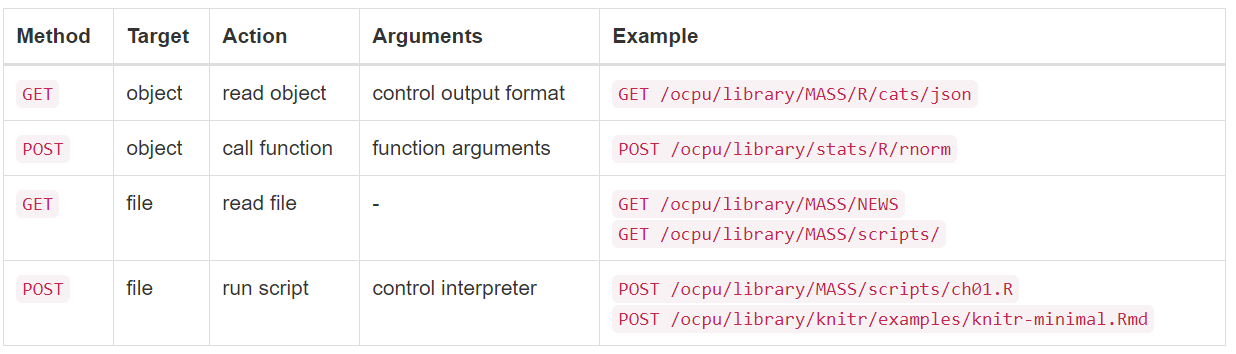
\includegraphics{pic/opencpu/p1.png}

\begin{Shaded}
\begin{Highlighting}[]
\CommentTok{# Get 举栗}
\NormalTok{curl http}\OperatorTok{:}\ErrorTok{//}\FloatTok{172.16}\NormalTok{.}\FloatTok{100.202}\OperatorTok{/}\NormalTok{ocpu}\OperatorTok{/}\NormalTok{library}\OperatorTok{/}\NormalTok{MASS}\OperatorTok{/}\NormalTok{data}\OperatorTok{/}\NormalTok{Boston}\OperatorTok{/}\NormalTok{json}
\NormalTok{curl http}\OperatorTok{:}\ErrorTok{//}\FloatTok{172.16}\NormalTok{.}\FloatTok{100.202}\OperatorTok{/}\NormalTok{ocpu}\OperatorTok{/}\NormalTok{library}\OperatorTok{/}\NormalTok{MASS}\OperatorTok{/}\NormalTok{NEWS}
\NormalTok{curl http}\OperatorTok{:}\ErrorTok{//}\FloatTok{172.16}\NormalTok{.}\FloatTok{100.202}\OperatorTok{/}\NormalTok{ocpu}\OperatorTok{/}\NormalTok{library}\OperatorTok{/}\NormalTok{MASS}\OperatorTok{/}\NormalTok{scripts}\OperatorTok{/}

\CommentTok{#Post 举栗 -X POST or -d "arg=value"}
\NormalTok{curl http}\OperatorTok{:}\ErrorTok{//}\FloatTok{172.16}\NormalTok{.}\FloatTok{100.202}\OperatorTok{/}\NormalTok{ocpu}\OperatorTok{/}\NormalTok{library}\OperatorTok{/}\NormalTok{MASS}\OperatorTok{/}\NormalTok{scripts}\OperatorTok{/}\NormalTok{ch01.R }\OperatorTok{-}\NormalTok{X POST}
\NormalTok{curl http}\OperatorTok{:}\ErrorTok{//}\FloatTok{172.16}\NormalTok{.}\FloatTok{100.202}\OperatorTok{/}\NormalTok{ocpu}\OperatorTok{/}\NormalTok{library}\OperatorTok{/}\NormalTok{stats}\OperatorTok{/}\NormalTok{R}\OperatorTok{/}\NormalTok{rnorm }\OperatorTok{-}\NormalTok{d }\StringTok{"n=10&mean=5"}

\end{Highlighting}
\end{Shaded}

\begin{center}\rule{0.5\linewidth}{\linethickness}\end{center}

Http状态码

这些是OpenCPU返回的常见状态代码,客户端应该能够解释这些状态代码

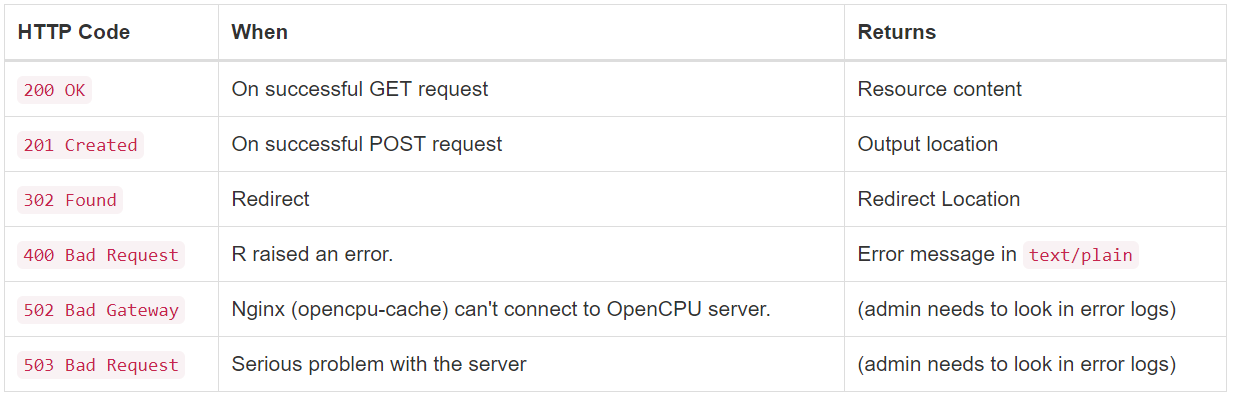
\includegraphics{pic/opencpu/p2.png}

\subsection{API 端点(EndPoints)}\label{api-endpoints}

\begin{center}\rule{0.5\linewidth}{\linethickness}\end{center}

The API Libraries

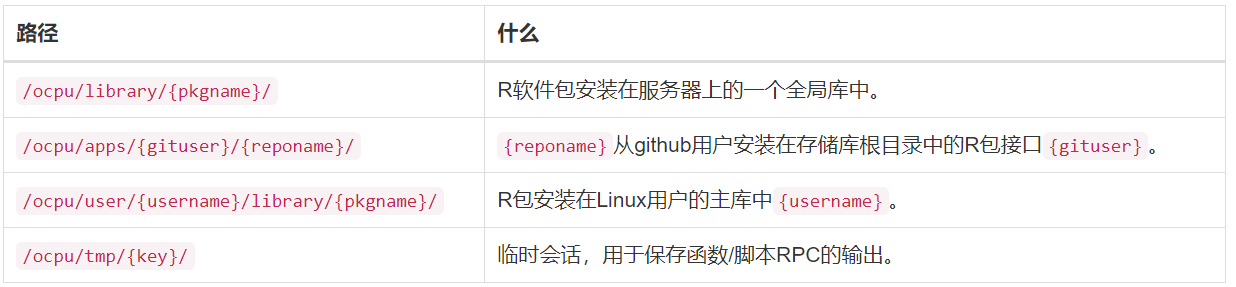
\includegraphics{pic/opencpu/p3.png}

\begin{Shaded}
\begin{Highlighting}[]
\CommentTok{#read packages 举栗}
\NormalTok{curl http}\OperatorTok{:}\ErrorTok{//}\FloatTok{172.16}\NormalTok{.}\FloatTok{100.202}\OperatorTok{/}\NormalTok{ocpu}\OperatorTok{/}\NormalTok{library}\OperatorTok{/}
\NormalTok{curl http}\OperatorTok{:}\ErrorTok{//}\FloatTok{172.16}\NormalTok{.}\FloatTok{100.202}\OperatorTok{/}\NormalTok{ocpu}\OperatorTok{/}\NormalTok{apps}\OperatorTok{/}\NormalTok{rwebapps}\OperatorTok{/}
\NormalTok{curl http}\OperatorTok{:}\ErrorTok{//}\FloatTok{172.16}\NormalTok{.}\FloatTok{100.202}\OperatorTok{/}\NormalTok{ocpu}\OperatorTok{/}\NormalTok{user}\OperatorTok{/}\NormalTok{jeroen}\OperatorTok{/}\NormalTok{library}\OperatorTok{/}

\CommentTok{#read session 举栗}
\NormalTok{curl http}\OperatorTok{:}\ErrorTok{//}\FloatTok{172.16}\NormalTok{.}\FloatTok{100.202}\OperatorTok{/}\NormalTok{ocpu}\OperatorTok{/}\NormalTok{tmp}\OperatorTok{/}\NormalTok{x2c5ab8d4d6}
\end{Highlighting}
\end{Shaded}

\begin{center}\rule{0.5\linewidth}{\linethickness}\end{center}

The R package API

\texttt{/\{package\}/}库都支持以下端点:

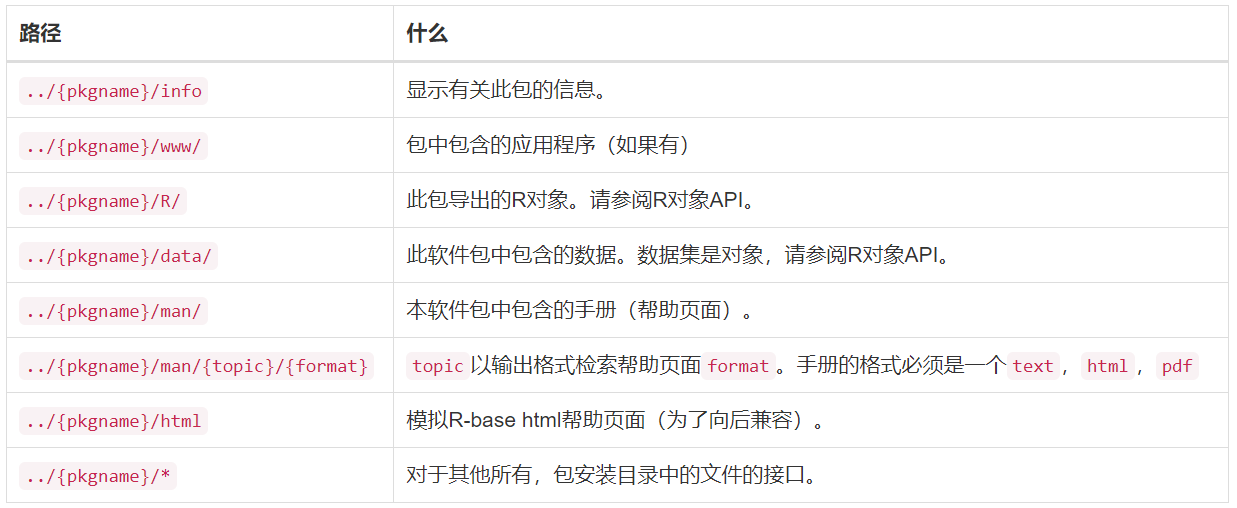
\includegraphics{pic/opencpu/p4.png}

\begin{Shaded}
\begin{Highlighting}[]
\CommentTok{#package info}
\NormalTok{curl http}\OperatorTok{:}\ErrorTok{//}\FloatTok{172.16}\NormalTok{.}\FloatTok{100.202}\OperatorTok{/}\NormalTok{ocpu}\OperatorTok{/}\NormalTok{library}\OperatorTok{/}\NormalTok{MASS}\OperatorTok{/}

\CommentTok{#package objects (mostly functions)}
\NormalTok{curl http}\OperatorTok{:}\ErrorTok{//}\FloatTok{172.16}\NormalTok{.}\FloatTok{100.202}\OperatorTok{/}\NormalTok{ocpu}\OperatorTok{/}\NormalTok{library}\OperatorTok{/}\NormalTok{MASS}\OperatorTok{/}\NormalTok{R}\OperatorTok{/}
\NormalTok{curl http}\OperatorTok{:}\ErrorTok{//}\FloatTok{172.16}\NormalTok{.}\FloatTok{100.202}\OperatorTok{/}\NormalTok{ocpu}\OperatorTok{/}\NormalTok{library}\OperatorTok{/}\NormalTok{MASS}\OperatorTok{/}\NormalTok{R}\OperatorTok{/}\NormalTok{rlm}\OperatorTok{/}\NormalTok{print}

\CommentTok{#package data objects}
\NormalTok{curl http}\OperatorTok{:}\ErrorTok{//}\FloatTok{172.16}\NormalTok{.}\FloatTok{100.202}\OperatorTok{/}\NormalTok{ocpu}\OperatorTok{/}\NormalTok{library}\OperatorTok{/}\NormalTok{MASS}\OperatorTok{/}\NormalTok{data}\OperatorTok{/}
\NormalTok{curl http}\OperatorTok{:}\ErrorTok{//}\FloatTok{172.16}\NormalTok{.}\FloatTok{100.202}\OperatorTok{/}\NormalTok{ocpu}\OperatorTok{/}\NormalTok{library}\OperatorTok{/}\NormalTok{MASS}\OperatorTok{/}\NormalTok{data}\OperatorTok{/}\NormalTok{housing}\OperatorTok{/}\NormalTok{json}

\CommentTok{#read manuals pages}
\NormalTok{curl http}\OperatorTok{:}\ErrorTok{//}\FloatTok{172.16}\NormalTok{.}\FloatTok{100.202}\OperatorTok{/}\NormalTok{ocpu}\OperatorTok{/}\NormalTok{library}\OperatorTok{/}\NormalTok{MASS}\OperatorTok{/}\NormalTok{man}\OperatorTok{/}
\NormalTok{curl http}\OperatorTok{:}\ErrorTok{//}\FloatTok{172.16}\NormalTok{.}\FloatTok{100.202}\OperatorTok{/}\NormalTok{ocpu}\OperatorTok{/}\NormalTok{library}\OperatorTok{/}\NormalTok{MASS}\OperatorTok{/}\NormalTok{man}\OperatorTok{/}\NormalTok{rlm}\OperatorTok{/}\NormalTok{text}
\NormalTok{curl http}\OperatorTok{:}\ErrorTok{//}\FloatTok{172.16}\NormalTok{.}\FloatTok{100.202}\OperatorTok{/}\NormalTok{ocpu}\OperatorTok{/}\NormalTok{library}\OperatorTok{/}\NormalTok{MASS}\OperatorTok{/}\NormalTok{man}\OperatorTok{/}\NormalTok{rlm}\OperatorTok{/}\NormalTok{html}
\NormalTok{curl http}\OperatorTok{:}\ErrorTok{//}\FloatTok{172.16}\NormalTok{.}\FloatTok{100.202}\OperatorTok{/}\NormalTok{ocpu}\OperatorTok{/}\NormalTok{library}\OperatorTok{/}\NormalTok{MASS}\OperatorTok{/}\NormalTok{man}\OperatorTok{/}\NormalTok{rlm}\OperatorTok{/}\NormalTok{pdf}

\CommentTok{#read files included with this package}
\NormalTok{curl http}\OperatorTok{:}\ErrorTok{//}\FloatTok{172.16}\NormalTok{.}\FloatTok{100.202}\OperatorTok{/}\NormalTok{ocpu}\OperatorTok{/}\NormalTok{library}\OperatorTok{/}\NormalTok{MASS}\OperatorTok{/}\NormalTok{scripts}\OperatorTok{/}
\NormalTok{curl http}\OperatorTok{:}\ErrorTok{//}\FloatTok{172.16}\NormalTok{.}\FloatTok{100.202}\OperatorTok{/}\NormalTok{ocpu}\OperatorTok{/}\NormalTok{library}\OperatorTok{/}\NormalTok{MASS}\OperatorTok{/}\NormalTok{scripts}\OperatorTok{/}\NormalTok{ch01.R}
\NormalTok{curl http}\OperatorTok{:}\ErrorTok{//}\FloatTok{172.16}\NormalTok{.}\FloatTok{100.202}\OperatorTok{/}\NormalTok{ocpu}\OperatorTok{/}\NormalTok{library}\OperatorTok{/}\NormalTok{MASS}\OperatorTok{/}\NormalTok{NEWS}

\CommentTok{#call a function (example from 'rlm' help page)}
\NormalTok{curl http}\OperatorTok{:}\ErrorTok{//}\FloatTok{172.16}\NormalTok{.}\FloatTok{100.202}\OperatorTok{/}\NormalTok{ocpu}\OperatorTok{/}\NormalTok{library}\OperatorTok{/}\NormalTok{MASS}\OperatorTok{/}\NormalTok{R}\OperatorTok{/}\NormalTok{rlm }\OperatorTok{-}\NormalTok{d }\StringTok{"formula=stack.loss ~ .&data=stackloss&psi=psi.bisquare"}

\CommentTok{#run R script}
\NormalTok{curl http}\OperatorTok{:}\ErrorTok{//}\FloatTok{172.16}\NormalTok{.}\FloatTok{100.202}\OperatorTok{/}\NormalTok{ocpu}\OperatorTok{/}\NormalTok{library}\OperatorTok{/}\NormalTok{MASS}\OperatorTok{/}\NormalTok{scripts}\OperatorTok{/}\NormalTok{ch01.R }\OperatorTok{-}\NormalTok{X POST}

\CommentTok{#read output (replace key with value returned from previous request)}
\NormalTok{curl http}\OperatorTok{:}\ErrorTok{//}\FloatTok{172.16}\NormalTok{.}\FloatTok{100.202}\OperatorTok{/}\NormalTok{ocpu}\OperatorTok{/}\NormalTok{tmp}\OperatorTok{/}\NormalTok{x0648ec526b}\OperatorTok{/}\NormalTok{R}\OperatorTok{/}\NormalTok{.val}\OperatorTok{/}\NormalTok{print}
\end{Highlighting}
\end{Shaded}

\begin{center}\rule{0.5\linewidth}{\linethickness}\end{center}

The R object API

\texttt{/R} API 用来读取R对象或者调用R的方法.

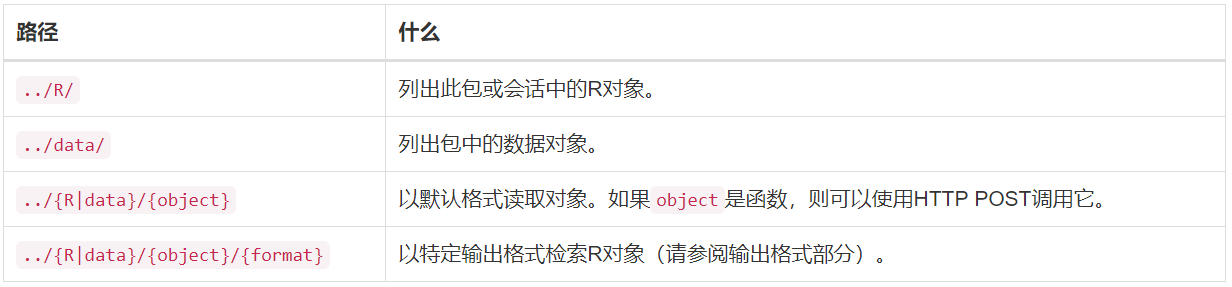
\includegraphics{pic/opencpu/p5.png}

\begin{Shaded}
\begin{Highlighting}[]
\CommentTok{#list objects and datasets from MASS}
\NormalTok{curl http}\OperatorTok{:}\ErrorTok{//}\FloatTok{172.16}\NormalTok{.}\FloatTok{100.202}\OperatorTok{/}\NormalTok{ocpu}\OperatorTok{/}\NormalTok{library}\OperatorTok{/}\NormalTok{MASS}\OperatorTok{/}\NormalTok{R}\OperatorTok{/}
\NormalTok{curl http}\OperatorTok{:}\ErrorTok{//}\FloatTok{172.16}\NormalTok{.}\FloatTok{100.202}\OperatorTok{/}\NormalTok{ocpu}\OperatorTok{/}\NormalTok{library}\OperatorTok{/}\NormalTok{MASS}\OperatorTok{/}\NormalTok{data}\OperatorTok{/}

\CommentTok{#retrieve objects}
\NormalTok{curl http}\OperatorTok{:}\ErrorTok{//}\FloatTok{172.16}\NormalTok{.}\FloatTok{100.202}\OperatorTok{/}\NormalTok{ocpu}\OperatorTok{/}\NormalTok{library}\OperatorTok{/}\NormalTok{MASS}\OperatorTok{/}\NormalTok{R}\OperatorTok{/}\NormalTok{truehist}\OperatorTok{/}\NormalTok{print}
\NormalTok{curl http}\OperatorTok{:}\ErrorTok{//}\FloatTok{172.16}\NormalTok{.}\FloatTok{100.202}\OperatorTok{/}\NormalTok{ocpu}\OperatorTok{/}\NormalTok{library}\OperatorTok{/}\NormalTok{MASS}\OperatorTok{/}\NormalTok{data}\OperatorTok{/}\NormalTok{bacteria}\OperatorTok{/}\NormalTok{print}
\NormalTok{curl http}\OperatorTok{:}\ErrorTok{//}\FloatTok{172.16}\NormalTok{.}\FloatTok{100.202}\OperatorTok{/}\NormalTok{ocpu}\OperatorTok{/}\NormalTok{library}\OperatorTok{/}\NormalTok{MASS}\OperatorTok{/}\NormalTok{data}\OperatorTok{/}\NormalTok{bacteria}\OperatorTok{/}\NormalTok{json}
\NormalTok{curl http}\OperatorTok{:}\ErrorTok{//}\FloatTok{172.16}\NormalTok{.}\FloatTok{100.202}\OperatorTok{/}\NormalTok{ocpu}\OperatorTok{/}\NormalTok{library}\OperatorTok{/}\NormalTok{MASS}\OperatorTok{/}\NormalTok{data}\OperatorTok{/}\NormalTok{bacteria}\OperatorTok{/}\NormalTok{csv}
\NormalTok{curl http}\OperatorTok{:}\ErrorTok{//}\FloatTok{172.16}\NormalTok{.}\FloatTok{100.202}\OperatorTok{/}\NormalTok{ocpu}\OperatorTok{/}\NormalTok{library}\OperatorTok{/}\NormalTok{MASS}\OperatorTok{/}\NormalTok{data}\OperatorTok{/}\NormalTok{bacteria}\OperatorTok{/}\NormalTok{rda}

\CommentTok{#call a function}
\NormalTok{curl http}\OperatorTok{:}\ErrorTok{//}\FloatTok{172.16}\NormalTok{.}\FloatTok{100.202}\OperatorTok{/}\NormalTok{ocpu}\OperatorTok{/}\NormalTok{library}\OperatorTok{/}\NormalTok{MASS}\OperatorTok{/}\NormalTok{R}\OperatorTok{/}\NormalTok{truehist }\OperatorTok{-}\NormalTok{d }\StringTok{"data=[1,3,7,4,2,4,2,6,23,13,5,2]"}
\end{Highlighting}
\end{Shaded}

\begin{center}\rule{0.5\linewidth}{\linethickness}\end{center}

The R session API

会话(session)是一个容器,用于保存从远程函数/脚本调用(RPC)创建的资源。

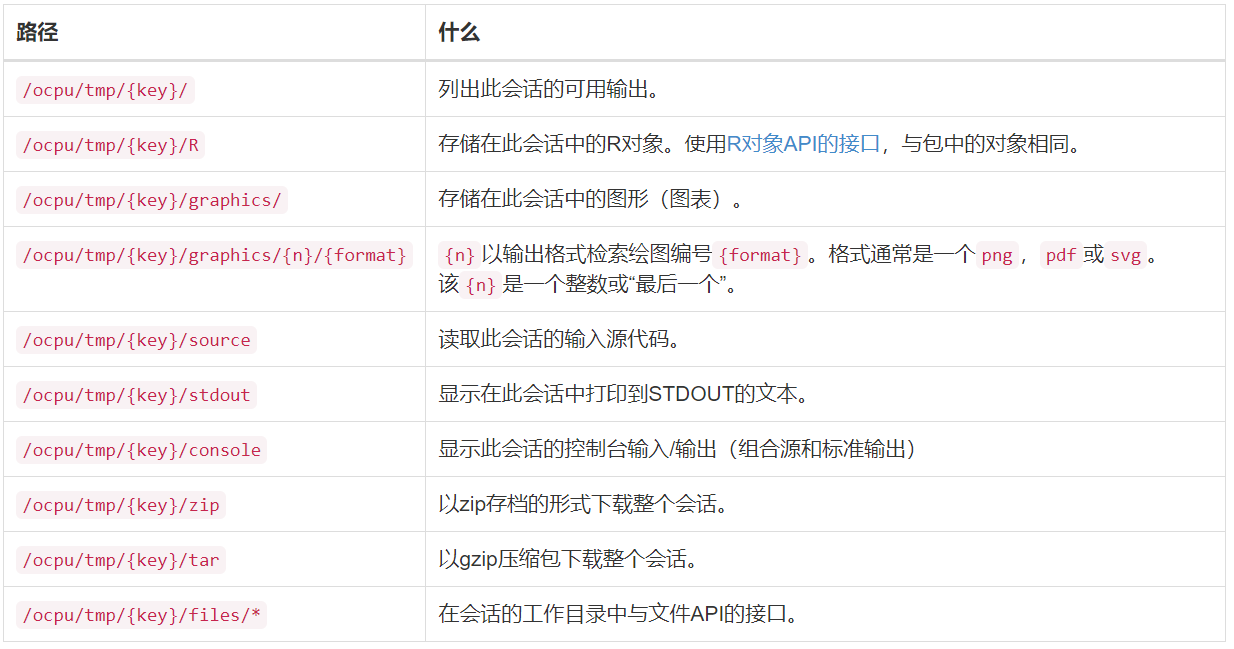
\includegraphics{pic/opencpu/p6.png}

\begin{Shaded}
\begin{Highlighting}[]
\CommentTok{#A POST will create a temporary session}
\CommentTok{#Use the returned key for the subsequent calls below}
\NormalTok{curl http}\OperatorTok{:}\ErrorTok{//}\FloatTok{172.16}\NormalTok{.}\FloatTok{100.202}\OperatorTok{/}\NormalTok{ocpu}\OperatorTok{/}\NormalTok{library}\OperatorTok{/}\NormalTok{MASS}\OperatorTok{/}\NormalTok{scripts}\OperatorTok{/}\NormalTok{ch01.R }\OperatorTok{-}\NormalTok{X POST}

\CommentTok{#Look at console input/output}
\NormalTok{curl http}\OperatorTok{:}\ErrorTok{//}\FloatTok{172.16}\NormalTok{.}\FloatTok{100.202}\OperatorTok{/}\NormalTok{ocpu}\OperatorTok{/}\NormalTok{tmp}\OperatorTok{/}\NormalTok{x05b85461}\OperatorTok{/}\NormalTok{console}\OperatorTok{/}\NormalTok{text}

\CommentTok{#We read session R objects}
\NormalTok{curl http}\OperatorTok{:}\ErrorTok{//}\FloatTok{172.16}\NormalTok{.}\FloatTok{100.202}\OperatorTok{/}\NormalTok{ocpu}\OperatorTok{/}\NormalTok{tmp}\OperatorTok{/}\NormalTok{x05b85461}\OperatorTok{/}
\NormalTok{curl http}\OperatorTok{:}\ErrorTok{//}\FloatTok{172.16}\NormalTok{.}\FloatTok{100.202}\OperatorTok{/}\NormalTok{ocpu}\OperatorTok{/}\NormalTok{tmp}\OperatorTok{/}\NormalTok{x05b85461}\OperatorTok{/}\NormalTok{R}\OperatorTok{/}
\NormalTok{curl http}\OperatorTok{:}\ErrorTok{//}\FloatTok{172.16}\NormalTok{.}\FloatTok{100.202}\OperatorTok{/}\NormalTok{ocpu}\OperatorTok{/}\NormalTok{tmp}\OperatorTok{/}\NormalTok{x05b85461}\OperatorTok{/}\NormalTok{R}\OperatorTok{/}\NormalTok{dd}\OperatorTok{/}\NormalTok{csv}
\NormalTok{curl http}\OperatorTok{:}\ErrorTok{//}\FloatTok{172.16}\NormalTok{.}\FloatTok{100.202}\OperatorTok{/}\NormalTok{ocpu}\OperatorTok{/}\NormalTok{tmp}\OperatorTok{/}\NormalTok{x05b85461}\OperatorTok{/}\NormalTok{R}\OperatorTok{/}\NormalTok{t.stat}\OperatorTok{/}\NormalTok{print}

\CommentTok{#Or even call a function}
\NormalTok{curl http}\OperatorTok{:}\ErrorTok{//}\FloatTok{172.16}\NormalTok{.}\FloatTok{100.202}\OperatorTok{/}\NormalTok{ocpu}\OperatorTok{/}\NormalTok{tmp}\OperatorTok{/}\NormalTok{x05b85461}\OperatorTok{/}\NormalTok{R}\OperatorTok{/}\NormalTok{t.stat }\OperatorTok{-}\NormalTok{d }\StringTok{"x=[1,0,0,1,1,1,0,1,1,0]"}

\CommentTok{#Download file from the working dir}
\NormalTok{curl http}\OperatorTok{:}\ErrorTok{//}\FloatTok{172.16}\NormalTok{.}\FloatTok{100.202}\OperatorTok{/}\NormalTok{ocpu}\OperatorTok{/}\NormalTok{tmp}\OperatorTok{/}\NormalTok{x05b85461}\OperatorTok{/}\NormalTok{files}\OperatorTok{/}\NormalTok{ch01.pdf}

\CommentTok{#Check sessionInfo}
\NormalTok{curl http}\OperatorTok{:}\ErrorTok{//}\FloatTok{172.16}\NormalTok{.}\FloatTok{100.202}\OperatorTok{/}\NormalTok{ocpu}\OperatorTok{/}\NormalTok{tmp}\OperatorTok{/}\NormalTok{x05b85461}\OperatorTok{/}\NormalTok{info}\OperatorTok{/}\NormalTok{print}
\end{Highlighting}
\end{Shaded}

\subsection{输入,输出:数据和格式}

\begin{center}\rule{0.5\linewidth}{\linethickness}\end{center}

R对象的输出格式

可以以各种输出格式检索任何R对象(包括记录的图形)

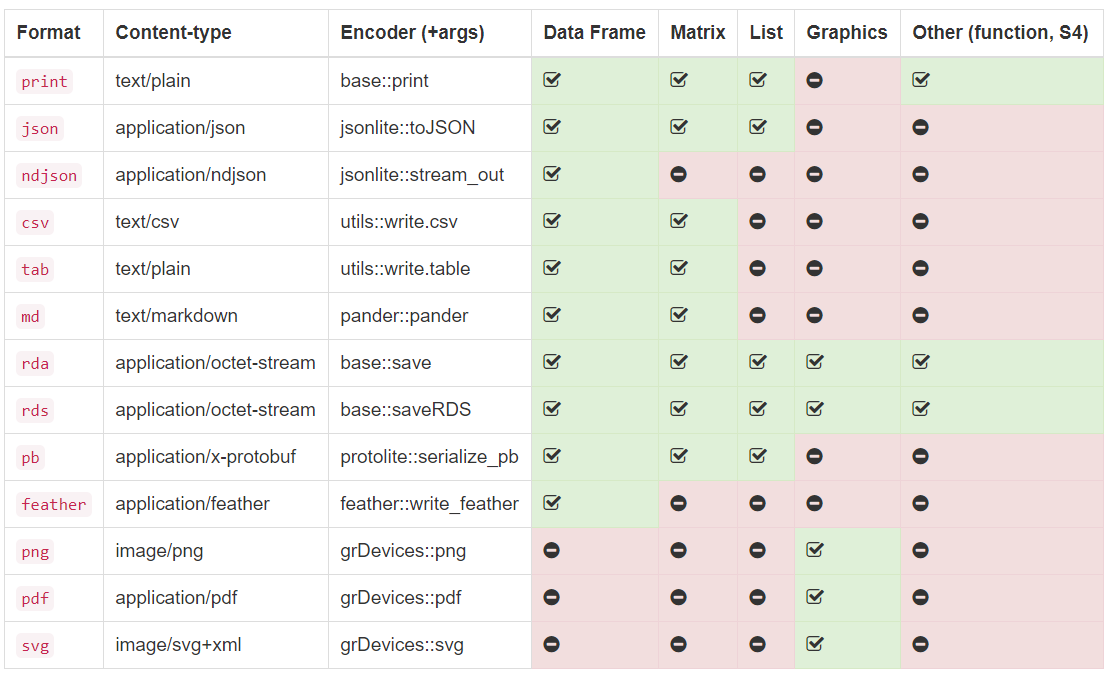
\includegraphics{pic/opencpu/p7.png}

\begin{Shaded}
\begin{Highlighting}[]
\CommentTok{#read R objects from packages.}
\NormalTok{curl http}\OperatorTok{:}\ErrorTok{//}\FloatTok{172.16}\NormalTok{.}\FloatTok{100.202}\OperatorTok{/}\NormalTok{ocpu}\OperatorTok{/}\NormalTok{library}\OperatorTok{/}\NormalTok{datasets}\OperatorTok{/}\NormalTok{R}\OperatorTok{/}\NormalTok{mtcars}\OperatorTok{/}\NormalTok{json?digits=}\DecValTok{0}
\NormalTok{curl http}\OperatorTok{:}\ErrorTok{//}\FloatTok{172.16}\NormalTok{.}\FloatTok{100.202}\OperatorTok{/}\NormalTok{ocpu}\OperatorTok{/}\NormalTok{library}\OperatorTok{/}\NormalTok{datasets}\OperatorTok{/}\NormalTok{R}\OperatorTok{/}\NormalTok{mtcars}\OperatorTok{/}\NormalTok{csv}
\NormalTok{curl http}\OperatorTok{:}\ErrorTok{//}\FloatTok{172.16}\NormalTok{.}\FloatTok{100.202}\OperatorTok{/}\NormalTok{ocpu}\OperatorTok{/}\NormalTok{library}\OperatorTok{/}\NormalTok{datasets}\OperatorTok{/}\NormalTok{R}\OperatorTok{/}\NormalTok{mtcars}\OperatorTok{/}\NormalTok{tab?sep=}\StringTok{"|"}
\NormalTok{curl http}\OperatorTok{:}\ErrorTok{//}\FloatTok{172.16}\NormalTok{.}\FloatTok{100.202}\OperatorTok{/}\NormalTok{ocpu}\OperatorTok{/}\NormalTok{library}\OperatorTok{/}\NormalTok{MASS}\OperatorTok{/}\NormalTok{R}\OperatorTok{/}\NormalTok{loglm}\OperatorTok{/}\NormalTok{print}
\end{Highlighting}
\end{Shaded}

\begin{Shaded}
\begin{Highlighting}[]
\CommentTok{#create a simple plot}
\NormalTok{curl http}\OperatorTok{:}\ErrorTok{//}\FloatTok{172.16}\NormalTok{.}\FloatTok{100.202}\OperatorTok{/}\NormalTok{ocpu}\OperatorTok{/}\NormalTok{library}\OperatorTok{/}\NormalTok{graphics}\OperatorTok{/}\NormalTok{R}\OperatorTok{/}\NormalTok{plot }\OperatorTok{-}\NormalTok{d }\StringTok{"x=cars"}

\CommentTok{#replace session id with returned one}
\NormalTok{curl http}\OperatorTok{:}\ErrorTok{//}\FloatTok{172.16}\NormalTok{.}\FloatTok{100.202}\OperatorTok{/}\NormalTok{ocpu}\OperatorTok{/}\NormalTok{tmp}\OperatorTok{/}\NormalTok{x0468b7ab}\OperatorTok{/}\NormalTok{graphics}\OperatorTok{/}\NormalTok{last}\OperatorTok{/}\NormalTok{png}
\NormalTok{curl http}\OperatorTok{:}\ErrorTok{//}\FloatTok{172.16}\NormalTok{.}\FloatTok{100.202}\OperatorTok{/}\NormalTok{ocpu}\OperatorTok{/}\NormalTok{tmp}\OperatorTok{/}\NormalTok{x0468b7ab}\OperatorTok{/}\NormalTok{graphics}\OperatorTok{/}\DecValTok{1}\OperatorTok{/}\NormalTok{png?width=}\DecValTok{1000}
\NormalTok{curl http}\OperatorTok{:}\ErrorTok{//}\FloatTok{172.16}\NormalTok{.}\FloatTok{100.202}\OperatorTok{/}\NormalTok{ocpu}\OperatorTok{/}\NormalTok{tmp}\OperatorTok{/}\NormalTok{x0468b7ab}\OperatorTok{/}\NormalTok{graphics}\OperatorTok{/}\NormalTok{last}\OperatorTok{/}\NormalTok{svg}
\NormalTok{curl http}\OperatorTok{:}\ErrorTok{//}\FloatTok{172.16}\NormalTok{.}\FloatTok{100.202}\OperatorTok{/}\NormalTok{ocpu}\OperatorTok{/}\NormalTok{tmp}\OperatorTok{/}\NormalTok{x0468b7ab}\OperatorTok{/}\NormalTok{graphics}\OperatorTok{/}\NormalTok{last}\OperatorTok{/}\NormalTok{pdf?width=}\DecValTok{8}
\end{Highlighting}
\end{Shaded}

\begin{center}\rule{0.5\linewidth}{\linethickness}\end{center}

R函数调用的参数格式(仅限HTTP POST)

调用函数时,我们需要传递参数。OpenCPU接受以下类型的参数

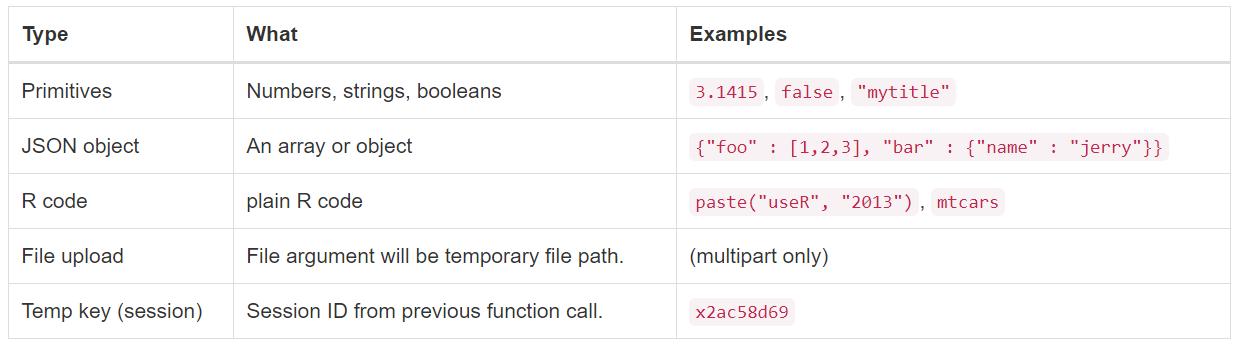
\includegraphics{pic/opencpu/p8.png}

执行函数功能时, Post的数据 (请求体)
可以使下面面的任意形式:\texttt{multipart/form-data},
\texttt{application/x-www-form-urlencoded}, \texttt{application/json}
或者 \texttt{application/x-protobuf}.
并非每个content-type都支持任何参数格式:

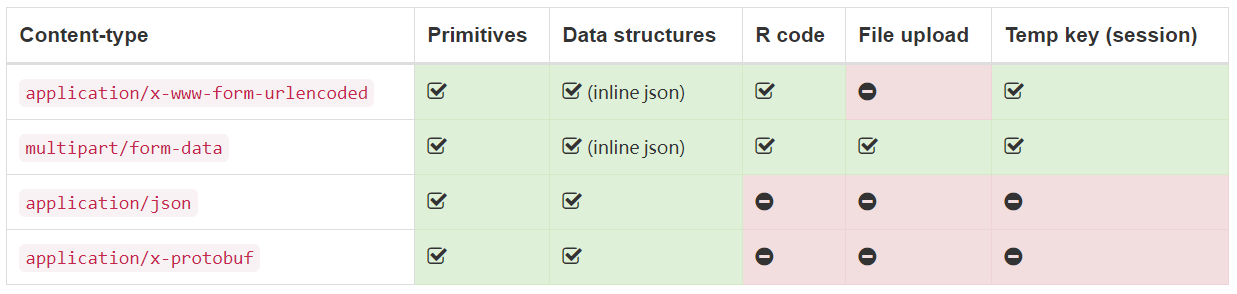
\includegraphics{pic/opencpu/p9.png}

\begin{Shaded}
\begin{Highlighting}[]
\CommentTok{#call some functions}
\NormalTok{curl http}\OperatorTok{:}\ErrorTok{//}\FloatTok{172.16}\NormalTok{.}\FloatTok{100.202}\OperatorTok{/}\NormalTok{ocpu}\OperatorTok{/}\NormalTok{library}\OperatorTok{/}\NormalTok{stats}\OperatorTok{/}\NormalTok{R}\OperatorTok{/}\NormalTok{rnorm }\OperatorTok{-}\NormalTok{d }\StringTok{"n=10&mean=5"}
\NormalTok{curl http}\OperatorTok{:}\ErrorTok{//}\FloatTok{172.16}\NormalTok{.}\FloatTok{100.202}\OperatorTok{/}\NormalTok{ocpu}\OperatorTok{/}\NormalTok{library}\OperatorTok{/}\NormalTok{graphics}\OperatorTok{/}\NormalTok{R}\OperatorTok{/}\NormalTok{hist }\OperatorTok{-}\NormalTok{d }\StringTok{"x=[2,3,2,3,4,3,3]&breaks=10"}
\NormalTok{curl http}\OperatorTok{:}\ErrorTok{//}\FloatTok{172.16}\NormalTok{.}\FloatTok{100.202}\OperatorTok{/}\NormalTok{ocpu}\OperatorTok{/}\NormalTok{library}\OperatorTok{/}\NormalTok{graphics}\OperatorTok{/}\NormalTok{R}\OperatorTok{/}\NormalTok{plot }\OperatorTok{-}\NormalTok{d }\StringTok{"x=cars&main='test'"}
\NormalTok{curl http}\OperatorTok{:}\ErrorTok{//}\FloatTok{172.16}\NormalTok{.}\FloatTok{100.202}\OperatorTok{/}\NormalTok{ocpu}\OperatorTok{/}\NormalTok{library}\OperatorTok{/}\NormalTok{base}\OperatorTok{/}\NormalTok{R}\OperatorTok{/}\NormalTok{identity }\OperatorTok{-}\NormalTok{d }\StringTok{"x=coef(lm(speed~dist, data=cars))"}
\end{Highlighting}
\end{Shaded}

\begin{Shaded}
\begin{Highlighting}[]
\CommentTok{#upload local file mydata.csv}
\NormalTok{curl http}\OperatorTok{:}\ErrorTok{//}\FloatTok{172.16}\NormalTok{.}\FloatTok{100.202}\OperatorTok{/}\NormalTok{ocpu}\OperatorTok{/}\NormalTok{library}\OperatorTok{/}\NormalTok{utils}\OperatorTok{/}\NormalTok{R}\OperatorTok{/}\NormalTok{read.csv }\OperatorTok{-}\NormalTok{F }\StringTok{"file=@mydata.csv"}

\CommentTok{#replace session id with returned one above}
\NormalTok{curl http}\OperatorTok{:}\ErrorTok{//}\FloatTok{172.16}\NormalTok{.}\FloatTok{100.202}\OperatorTok{/}\NormalTok{ocpu}\OperatorTok{/}\NormalTok{tmp}\OperatorTok{/}\NormalTok{x067b4172}\OperatorTok{/}\NormalTok{R}\OperatorTok{/}\NormalTok{.val}\OperatorTok{/}\NormalTok{print}
\NormalTok{curl http}\OperatorTok{:}\ErrorTok{//}\FloatTok{172.16}\NormalTok{.}\FloatTok{100.202}\OperatorTok{/}\NormalTok{ocpu}\OperatorTok{/}\NormalTok{library}\OperatorTok{/}\NormalTok{base}\OperatorTok{/}\NormalTok{R}\OperatorTok{/}\NormalTok{summary }\OperatorTok{-}\NormalTok{d }\StringTok{"object=x067b4172"}
\end{Highlighting}
\end{Shaded}

\begin{Shaded}
\begin{Highlighting}[]
\CommentTok{#post arguments in json}
\NormalTok{curl http}\OperatorTok{:}\ErrorTok{//}\NormalTok{cloud.opencpu.org}\OperatorTok{/}\NormalTok{ocpu}\OperatorTok{/}\NormalTok{library}\OperatorTok{/}\NormalTok{stats}\OperatorTok{/}\NormalTok{R}\OperatorTok{/}\NormalTok{rnorm \textbackslash{}}
\OperatorTok{-}\NormalTok{H }\StringTok{"Content-Type: application/json"} \OperatorTok{-}\NormalTok{d }\StringTok{'\{"n":10, "mean": 10, "sd":10\}'}
\end{Highlighting}
\end{Shaded}

\begin{center}\rule{0.5\linewidth}{\linethickness}\end{center}

运行脚本和可重现的文档

我们可以通过对文件执行HTTP
POST来运行脚本。该脚本根据其(不区分大小写)文件扩展名进行解释。任何HTTP
POST参数都会传递给解释函数。支持以下类型:

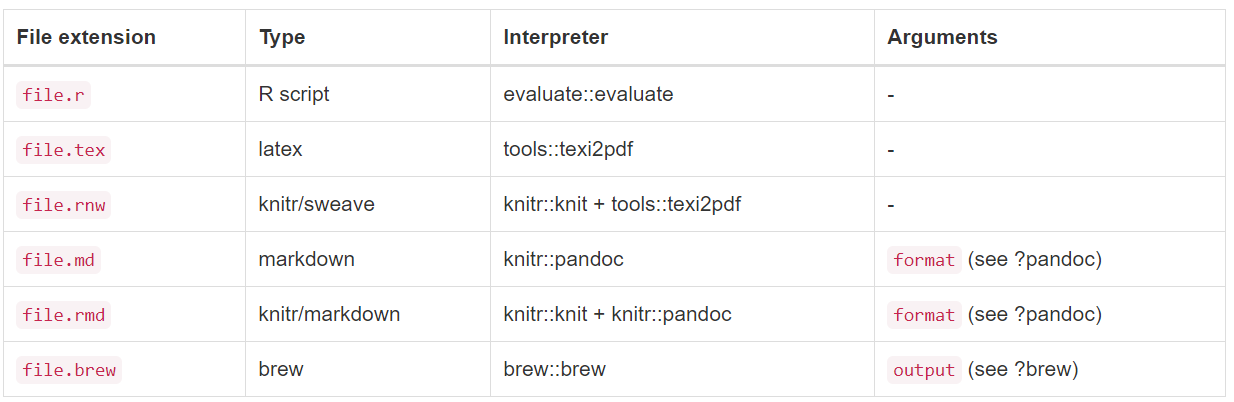
\includegraphics{pic/opencpu/p10.png}

\begin{Shaded}
\begin{Highlighting}[]
\CommentTok{#run scripts which exist in packages}
\NormalTok{curl http}\OperatorTok{:}\ErrorTok{//}\FloatTok{172.16}\NormalTok{.}\FloatTok{100.202}\OperatorTok{/}\NormalTok{ocpu}\OperatorTok{/}\NormalTok{library}\OperatorTok{/}\NormalTok{MASS}\OperatorTok{/}\NormalTok{scripts}\OperatorTok{/}\NormalTok{ch01.R }\OperatorTok{-}\NormalTok{X POST}
\NormalTok{curl http}\OperatorTok{:}\ErrorTok{//}\FloatTok{172.16}\NormalTok{.}\FloatTok{100.202}\OperatorTok{/}\NormalTok{ocpu}\OperatorTok{/}\NormalTok{library}\OperatorTok{/}\NormalTok{brew}\OperatorTok{/}\NormalTok{featurefull.brew }\OperatorTok{-}\NormalTok{X POST}
\NormalTok{curl http}\OperatorTok{:}\ErrorTok{//}\FloatTok{172.16}\NormalTok{.}\FloatTok{100.202}\OperatorTok{/}\NormalTok{ocpu}\OperatorTok{/}\NormalTok{library}\OperatorTok{/}\NormalTok{brew}\OperatorTok{/}\NormalTok{brew}\OperatorTok{-}\NormalTok{test}\OperatorTok{-}\FloatTok{2.}\NormalTok{brew }\OperatorTok{-}\NormalTok{d }\StringTok{"output=output.html"}
\NormalTok{curl http}\OperatorTok{:}\ErrorTok{//}\FloatTok{172.16}\NormalTok{.}\FloatTok{100.202}\OperatorTok{/}\NormalTok{ocpu}\OperatorTok{/}\NormalTok{library}\OperatorTok{/}\NormalTok{knitr}\OperatorTok{/}\NormalTok{examples}\OperatorTok{/}\NormalTok{knitr}\OperatorTok{-}\NormalTok{minimal.Rmd }\OperatorTok{-}\NormalTok{X POST}
\NormalTok{curl http}\OperatorTok{:}\ErrorTok{//}\FloatTok{172.16}\NormalTok{.}\FloatTok{100.202}\OperatorTok{/}\NormalTok{ocpu}\OperatorTok{/}\NormalTok{library}\OperatorTok{/}\NormalTok{knitr}\OperatorTok{/}\NormalTok{examples}\OperatorTok{/}\NormalTok{knitr}\OperatorTok{-}\NormalTok{minimal.Rmd }\OperatorTok{-}\NormalTok{d }\StringTok{"format=docx"}
\NormalTok{curl http}\OperatorTok{:}\ErrorTok{//}\FloatTok{172.16}\NormalTok{.}\FloatTok{100.202}\OperatorTok{/}\NormalTok{ocpu}\OperatorTok{/}\NormalTok{library}\OperatorTok{/}\NormalTok{knitr}\OperatorTok{/}\NormalTok{examples}\OperatorTok{/}\NormalTok{knitr}\OperatorTok{-}\NormalTok{minimal.Rmd }\OperatorTok{-}\NormalTok{d }\StringTok{"format=html"}
\NormalTok{curl http}\OperatorTok{:}\ErrorTok{//}\FloatTok{172.16}\NormalTok{.}\FloatTok{100.202}\OperatorTok{/}\NormalTok{ocpu}\OperatorTok{/}\NormalTok{library}\OperatorTok{/}\NormalTok{knitr}\OperatorTok{/}\NormalTok{examples}\OperatorTok{/}\NormalTok{knitr}\OperatorTok{-}\NormalTok{minimal.Rnw}
\end{Highlighting}
\end{Shaded}

\begin{center}\rule{0.5\linewidth}{\linethickness}\end{center}

JSON I / O RPC(又名数据处理单元)

对于客户端只对JSON格式的函数调用的输出数据感兴趣的常见特殊情况,可以使用后置修复HTTP
POST请求URL
/json。在这种情况下,成功调用将返回状态200(而不是201),并且响应主体直接包含JSON中返回的对象;
无需额外的GET请求。

\begin{Shaded}
\begin{Highlighting}[]
\NormalTok{curl http}\OperatorTok{:}\ErrorTok{//}\NormalTok{cloud.opencpu.org}\OperatorTok{/}\NormalTok{ocpu}\OperatorTok{/}\NormalTok{library}\OperatorTok{/}\NormalTok{stats}\OperatorTok{/}\NormalTok{R}\OperatorTok{/}\NormalTok{rnorm}\OperatorTok{/}\NormalTok{json }\OperatorTok{-}\NormalTok{d n=}\DecValTok{2}
\NormalTok{[}
\OperatorTok{-}\FloatTok{1.2804}\NormalTok{,}
\OperatorTok{-}\FloatTok{0.75013}
\NormalTok{]}
\end{Highlighting}
\end{Shaded}

我们可以将它与application/jsonR函数上的完整JSON RPC 的请求内容类型相结合

\begin{Shaded}
\begin{Highlighting}[]
\NormalTok{curl http}\OperatorTok{:}\ErrorTok{//}\NormalTok{cloud.opencpu.org}\OperatorTok{/}\NormalTok{ocpu}\OperatorTok{/}\NormalTok{library}\OperatorTok{/}\NormalTok{stats}\OperatorTok{/}\NormalTok{R}\OperatorTok{/}\NormalTok{rnorm}\OperatorTok{/}\NormalTok{json \textbackslash{}}
\OperatorTok{-}\NormalTok{H }\StringTok{"Content-Type: application/json"} \OperatorTok{-}\NormalTok{d }\StringTok{'\{"n":3, "mean": 10, "sd":10\}'}
\NormalTok{[}
\FloatTok{4.9829}\NormalTok{,}
\FloatTok{6.3104}\NormalTok{,}
\FloatTok{11.411}
\NormalTok{]}
\end{Highlighting}
\end{Shaded}

上面的请求调用以下R函数调用:

\begin{Shaded}
\begin{Highlighting}[]
\KeywordTok{library}\NormalTok{(jsonlite)}
\NormalTok{args <-}\StringTok{ }\KeywordTok{fromJSON}\NormalTok{(}\StringTok{'\{"n":3, "mean": 10, "sd":10\}'}\NormalTok{)}
\NormalTok{output <-}\StringTok{ }\KeywordTok{do.call}\NormalTok{(stats}\OperatorTok{::}\NormalTok{rnorm, args)}
\KeywordTok{toJSON}\NormalTok{(output)}
\end{Highlighting}
\end{Shaded}

在这种情况下,相当于:

\begin{Shaded}
\begin{Highlighting}[]
\KeywordTok{rnorm}\NormalTok{(}\DataTypeTok{n=}\DecValTok{3}\NormalTok{, }\DataTypeTok{mean=}\DecValTok{10}\NormalTok{, }\DataTypeTok{sd=}\DecValTok{10}\NormalTok{)}
\end{Highlighting}
\end{Shaded}

\subsection{其他功能}

\begin{center}\rule{0.5\linewidth}{\linethickness}\end{center}

OpenCPU应用程序

OpenCPU应用程序是包含在R包中的静态网页(html,css,js)。它们通过OpenCPU
API连接此包中的R函数。按照惯例,这些应用程序放在\texttt{/inst/www/}R源包的目录中。有关\href{https://www.opencpu.org/apps.html}{应用页面}的更多信息,请参阅。

\begin{Shaded}
\begin{Highlighting}[]
\KeywordTok{rnorm}\NormalTok{(}\DataTypeTok{n=}\DecValTok{3}\NormalTok{, }\DataTypeTok{mean=}\DecValTok{10}\NormalTok{, }\DataTypeTok{sd=}\DecValTok{10}\NormalTok{)}
\end{Highlighting}
\end{Shaded}

\begin{center}\rule{0.5\linewidth}{\linethickness}\end{center}

Github CI Hook

OpenCPU云服务器包括对持续集成(CI)的支持。因此,每次将提交推送到主分支时,可以将Github存储库配置为在OpenCPU服务器上自动安装程序包。要利用此功能,需要:

\begin{enumerate}
\def\labelenumi{\arabic{enumi}.}
\tightlist
\item
  R源包位于存储库的根目录中。\href{https://github.com/rwebapps/appdemo}{(例)}
\item
  Github用户帐户有一个公共电子邮件地址
\end{enumerate}

要设置CI,\texttt{/ocpu/webhook}请在Github存储库中将服务器的URL
添加为``WebHook''。例如,要使用公共演示服务器,请添加带有以下URL的webhook(您可以保持Content-type和Secret字段不变)

\begin{Shaded}
\begin{Highlighting}[]
\NormalTok{https}\OperatorTok{:}\ErrorTok{//}\NormalTok{cloud.opencpu.org}\OperatorTok{/}\NormalTok{ocpu}\OperatorTok{/}\NormalTok{webhook}
\end{Highlighting}
\end{Shaded}

要触发build,请将提交推送到主分支。build将显示在您的github
webhook页面中的Recent
Deliveries下,如果安装成功,您应该收到一封电子邮件(在您的垃圾邮件文件夹中)。如果是,则该程序包将直接可用于\texttt{/ocpu/apps/\{username\}/\{package\}/}服务器上的远程使用。

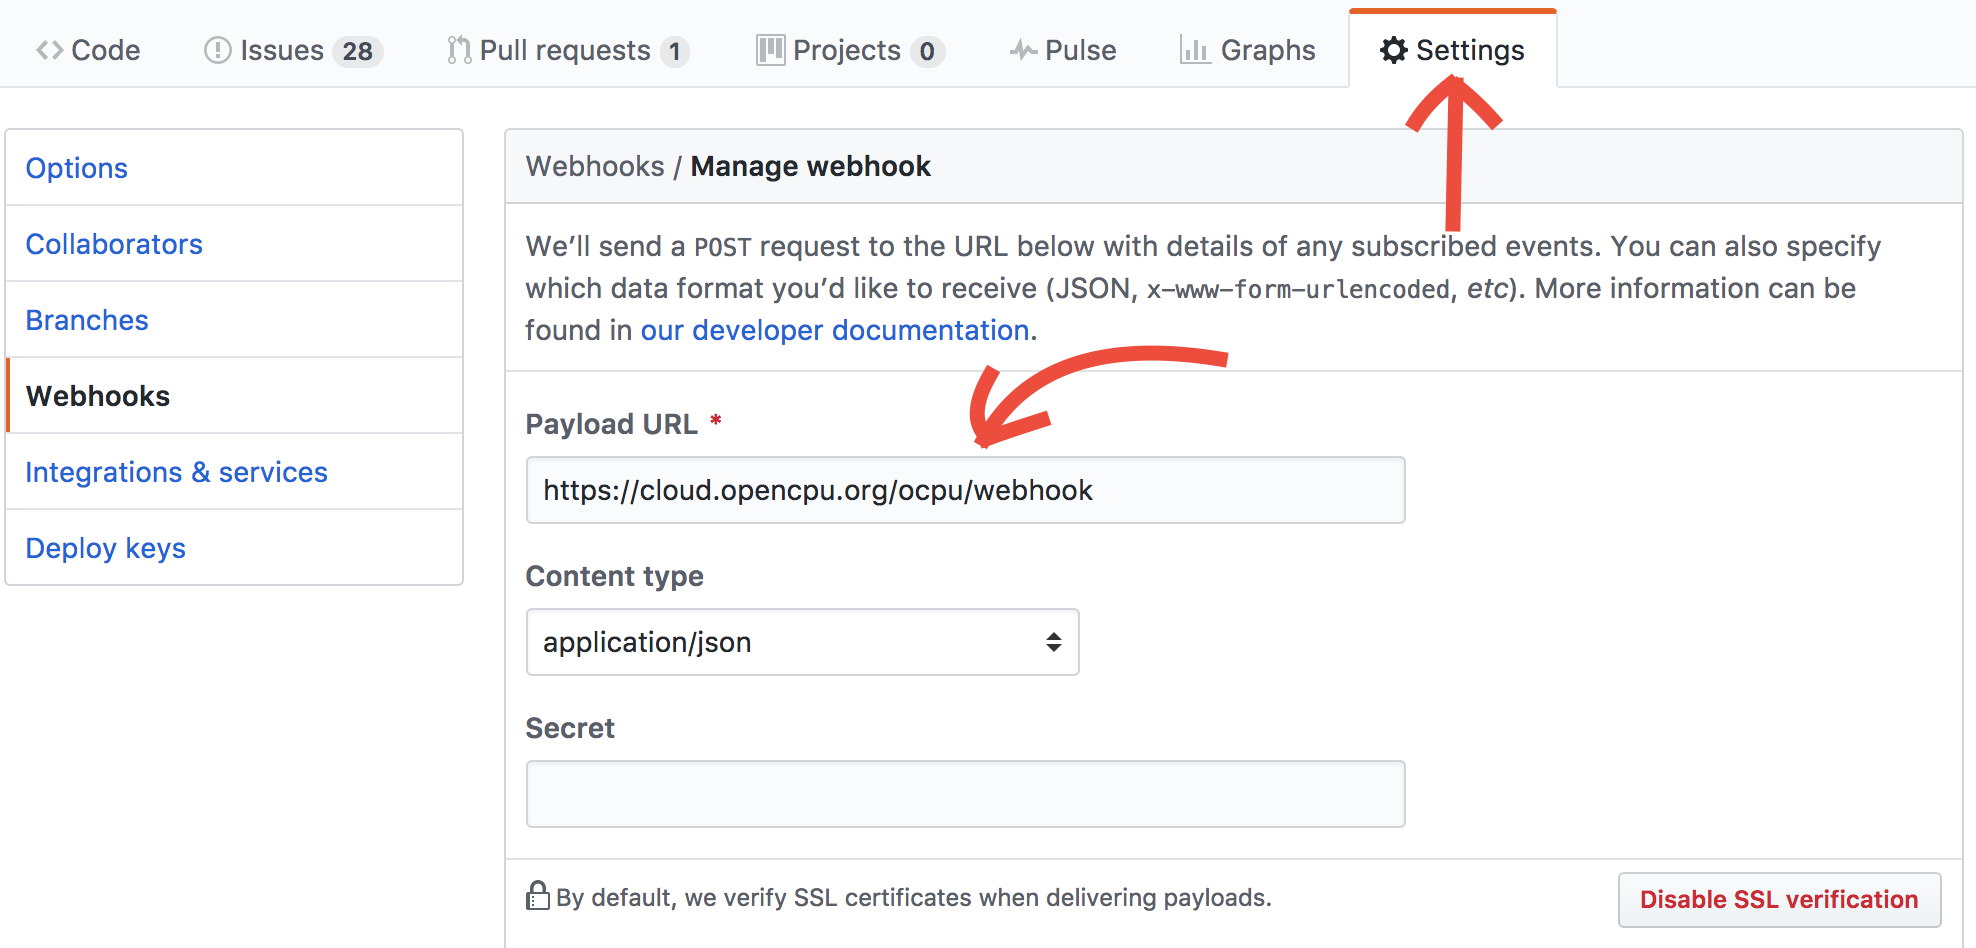
\includegraphics{pic/opencpu/p11.png}

如果您使用的是公共服务器,则该程序包也可以通过\texttt{https://\{yourname\}.ocpu.io/\{package\}/}。如果您正在运行自己的OpenCPU云服务器,则必须配置SMTP服务器才能使电子邮件通知正常工作。

\section{XGBoost模型部署实例}\label{xgboost}

本节将基于垃圾邮件的分类任务,训练一个XGBoost模型,基于训练的XGBoost模型构建一个R包,该R包的功能用于预测一封邮件是垃圾邮件的概率,并构建一个前端的页面,测试前端页面在opencpu中是可用的。其步骤如下:

\subsection{训练模型}

\begin{Shaded}
\begin{Highlighting}[]
\KeywordTok{library}\NormalTok{(xgboost)}
\KeywordTok{library}\NormalTok{(ElemStatLearn)}
\CommentTok{# 用于构建R包使用}
\NormalTok{data <-}\StringTok{ }\KeywordTok{save}\NormalTok{(spam,}\DataTypeTok{file=}\StringTok{'mail_data.rda'}\NormalTok{)}

\NormalTok{x =}\StringTok{ }\KeywordTok{as.matrix}\NormalTok{(spam[, }\OperatorTok{-}\KeywordTok{ncol}\NormalTok{(spam)])}
\NormalTok{y =}\StringTok{ }\KeywordTok{as.numeric}\NormalTok{(spam}\OperatorTok{$}\NormalTok{spam) }\OperatorTok{-}\StringTok{ }\DecValTok{1}
\NormalTok{xgbmodel =}\StringTok{ }\KeywordTok{xgboost}\NormalTok{(}\DataTypeTok{data =}\NormalTok{ x, }\DataTypeTok{label =}\NormalTok{ y, }\DataTypeTok{nrounds =} \DecValTok{5}\NormalTok{, }\DataTypeTok{objective =} \StringTok{'binary:logistic'}\NormalTok{)}
\CommentTok{# 这里模型保存的路径可以自己设置}
\CommentTok{# 保存的训练模型用于构建R包}
\KeywordTok{save}\NormalTok{(xgbmodel, }\DataTypeTok{file=}\StringTok{"xgb.rda"}\NormalTok{)}

\NormalTok{xgb_model <-}\StringTok{ }\KeywordTok{load}\NormalTok{(}\StringTok{"xgb.rda"}\NormalTok{)}
\NormalTok{xgbmodel}

\NormalTok{data_spam <-}\StringTok{ }\KeywordTok{as.matrix}\NormalTok{(spam[}\DecValTok{1}\NormalTok{, }\OperatorTok{-}\KeywordTok{ncol}\NormalTok{(spam)])}
\NormalTok{pred <-}\StringTok{ }\KeywordTok{predict}\NormalTok{(xgbmodel,data_spam)}
\CommentTok{# pred <- xgboost:::predict.xgb.Booster(object = xgbmodel, newdata = data_spam)}
\end{Highlighting}
\end{Shaded}

\subsection{构建R包}\label{r}

关于R包的构建,本教程不做详细的介绍,如果个人感兴趣可以参考R官网中的教程或Hadley
Wickham的\href{http://r-pkgs.had.co.nz/}{《R packages》}

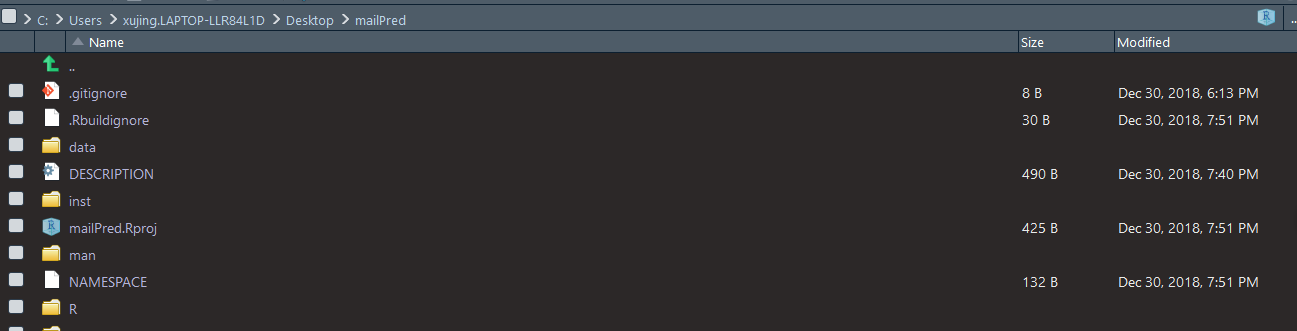
\includegraphics{pic/opencpu/p12.png}

\begin{Shaded}
\begin{Highlighting}[]
\CommentTok{#' @title Mail predict test for opencpu}
\CommentTok{#' @description Mail predict test for opencpu.}
\CommentTok{#' @name mailPred}
\CommentTok{#' @aliases mailPred}
\CommentTok{#' @author Xu Jing}
\CommentTok{#' @usage mailPreds(id)}
\CommentTok{#' @param id The row of mial data}
\CommentTok{#'}
\CommentTok{#' @import xgboost}
\CommentTok{#' @import jsonlite}
\CommentTok{#' @import stats}
\CommentTok{#' @import utils}
\CommentTok{#'}
\CommentTok{#' @export mailPreds}
\NormalTok{mailPreds <-}\StringTok{ }\ControlFlowTok{function}\NormalTok{(}\DataTypeTok{id =} \StringTok{'1'}\NormalTok{) \{}

  \KeywordTok{message}\NormalTok{(}\StringTok{"XGBoost model test on opencpu!"}\NormalTok{)}

\NormalTok{  spam <-}\StringTok{ }\OtherTok{NULL}
\NormalTok{  xgbmodel <-}\StringTok{ }\OtherTok{NULL}

\NormalTok{  spam_path <-}\StringTok{ }\KeywordTok{system.file}\NormalTok{(}\StringTok{"extdata"}\NormalTok{, }\StringTok{"mail_data.rda"}\NormalTok{, }\DataTypeTok{package =} \StringTok{"mailPred"}\NormalTok{)}
\NormalTok{  xgbmodel_path <-}\StringTok{ }\KeywordTok{system.file}\NormalTok{(}\StringTok{"extdata"}\NormalTok{, }\StringTok{"xgb.rda"}\NormalTok{, }\DataTypeTok{package =} \StringTok{"mailPred"}\NormalTok{)}

\NormalTok{  data_spam <-}\StringTok{ }\KeywordTok{load}\NormalTok{(spam_path)}
\NormalTok{  model_xgb <-}\StringTok{ }\KeywordTok{load}\NormalTok{(xgbmodel_path)}

\NormalTok{  x =}\StringTok{ }\KeywordTok{as.matrix}\NormalTok{(spam[}\KeywordTok{as.integer}\NormalTok{(id), }\OperatorTok{-}\KeywordTok{ncol}\NormalTok{(spam)])}
  \CommentTok{# y = as.numeric(spam[as.integer(id), ncol(spam)]) - 1}
\NormalTok{  pred <-}\StringTok{ }\KeywordTok{predict}\NormalTok{(xgbmodel,x)}
  \CommentTok{# print(spam)}

  \KeywordTok{return}\NormalTok{(}\KeywordTok{list}\NormalTok{(}\DataTypeTok{class =}\NormalTok{ pred,}\DataTypeTok{id=}\NormalTok{id))}
\NormalTok{\}}
\end{Highlighting}
\end{Shaded}

\begin{Shaded}
\begin{Highlighting}[]
\CommentTok{# DESCRIPTION}

\NormalTok{Package}\OperatorTok{:}\StringTok{ }\NormalTok{mailPred}
\NormalTok{Type}\OperatorTok{:}\StringTok{ }\NormalTok{Package}
\NormalTok{Title}\OperatorTok{:}\StringTok{ }\NormalTok{XGBoost Predict Mail}
\NormalTok{Version}\OperatorTok{:}\StringTok{ }\FloatTok{0.1}\NormalTok{.}\DecValTok{0}
\NormalTok{Author}\OperatorTok{:}\StringTok{ }\NormalTok{XuJing}
\NormalTok{Maintainer}\OperatorTok{:}\StringTok{ }\NormalTok{XuJing }\OperatorTok{<}\DecValTok{274762204}\OperatorTok{@}\NormalTok{qq.com}\OperatorTok{>}
\NormalTok{Description}\OperatorTok{:}\StringTok{ }\NormalTok{Mail predict test }\ControlFlowTok{for}\NormalTok{ opencpu.}
\NormalTok{License}\OperatorTok{:}\StringTok{ }\KeywordTok{GPL}\NormalTok{ (}\OperatorTok{>=}\StringTok{ }\DecValTok{2}\NormalTok{)}
\NormalTok{Encoding}\OperatorTok{:}\StringTok{ }\NormalTok{UTF}\OperatorTok{-}\DecValTok{8}
\NormalTok{LazyData}\OperatorTok{:}\StringTok{ }\NormalTok{false}
\NormalTok{Date}\OperatorTok{:}\StringTok{ }\DecValTok{2018}\OperatorTok{-}\DecValTok{12}\OperatorTok{-}\DecValTok{30}
\NormalTok{URL}\OperatorTok{:}\StringTok{ }\NormalTok{https}\OperatorTok{:}\ErrorTok{//}\NormalTok{github.com}\OperatorTok{/}\NormalTok{DataXujing}\OperatorTok{/}\NormalTok{mailPred}
\NormalTok{BugReports}\OperatorTok{:}\StringTok{ }\NormalTok{https}\OperatorTok{:}\ErrorTok{//}\NormalTok{github.com}\OperatorTok{/}\NormalTok{DataXujing}\OperatorTok{/}\NormalTok{mailPred}\OperatorTok{/}\NormalTok{issues}
\NormalTok{RoxygenNote}\OperatorTok{:}\StringTok{ }\FloatTok{6.1}\NormalTok{.}\DecValTok{1}
\NormalTok{Depends}\OperatorTok{:}\StringTok{ }\KeywordTok{R}\NormalTok{ (}\OperatorTok{>=}\StringTok{ }\FloatTok{3.4}\NormalTok{.}\DecValTok{0}\NormalTok{)}
\NormalTok{Imports}\OperatorTok{:}\StringTok{ }\NormalTok{xgboost,jsonlite,stats,utils}
\NormalTok{Suggests}\OperatorTok{:}\StringTok{ }\NormalTok{rmarkdown, knitr}
\NormalTok{VignetteBuilder}\OperatorTok{:}\StringTok{ }\NormalTok{knitr}
\end{Highlighting}
\end{Shaded}

\subsection{编译R包并安装}\label{r}

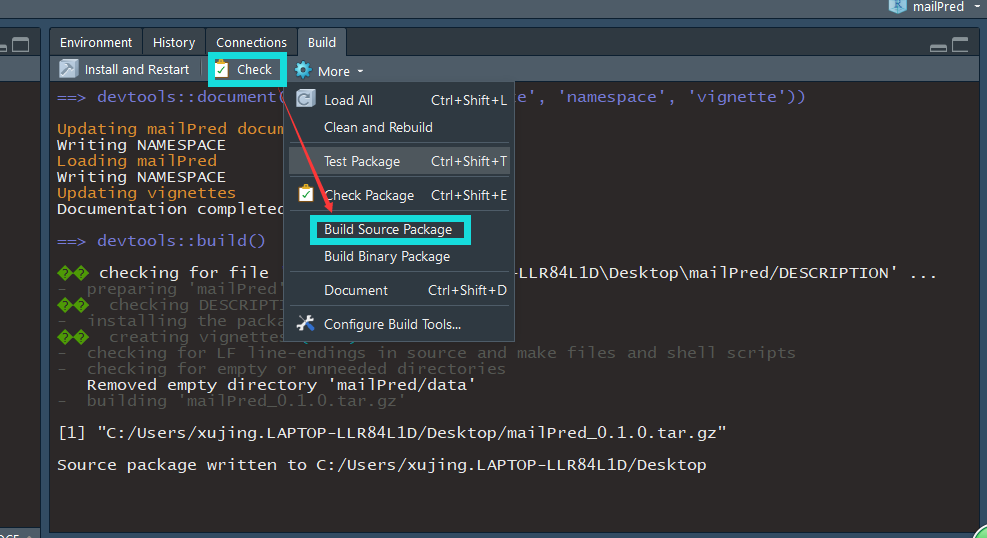
\includegraphics{pic/opencpu/p13.png}

\begin{itemize}
\tightlist
\item
  Rstudio中离线安装
\end{itemize}

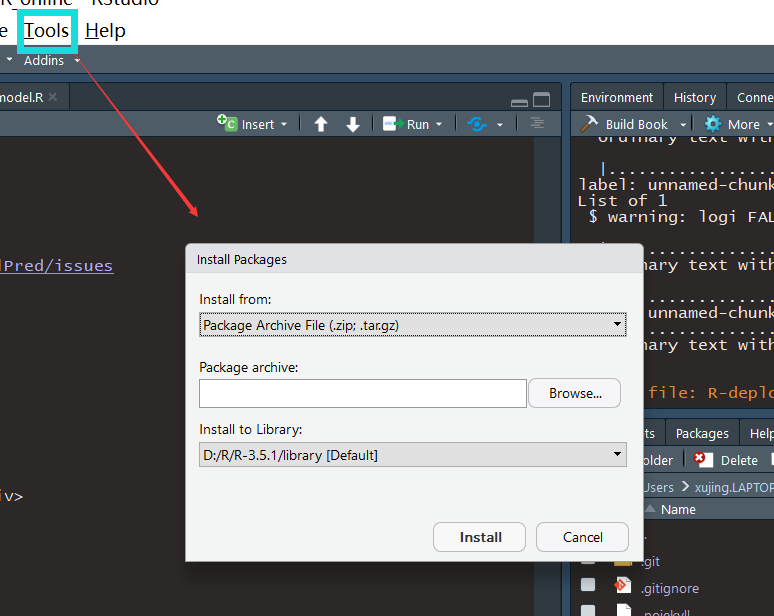
\includegraphics{pic/opencpu/p14.png}

\begin{itemize}
\tightlist
\item
  Ubuntu中离线安装
\end{itemize}

\begin{Shaded}
\begin{Highlighting}[]
\NormalTok{R CMD INSTALL mailPred_}\FloatTok{0.1}\NormalTok{.}\FloatTok{0.}\NormalTok{tar.gz}
\end{Highlighting}
\end{Shaded}

\subsection{opencpu的一些配置}\label{opencpu}

修改opencup服务参数,文件位于
\texttt{/etc/opencpu/server.conf},增加预加载的包

\begin{Shaded}
\begin{Highlighting}[]
\StringTok{"preload"}\OperatorTok{:}\StringTok{ }\NormalTok{[}\StringTok{"jsonlite"}\NormalTok{,}\StringTok{"xgboost"}\NormalTok{,}\StringTok{"glmnet"}\NormalTok{,}\StringTok{"mailPred"}\NormalTok{,}\StringTok{"ocputest"}\NormalTok{]}
\end{Highlighting}
\end{Shaded}

\subsection{本地opencpu服务测试}\label{opencpu}

\begin{Shaded}
\begin{Highlighting}[]
\KeywordTok{library}\NormalTok{(opencpu)}
\KeywordTok{ocpu_start_server}\NormalTok{(}\DataTypeTok{root=}\StringTok{'xj'}\NormalTok{)}
\end{Highlighting}
\end{Shaded}

\begin{Shaded}
\begin{Highlighting}[]
\NormalTok{http}\OperatorTok{:}\ErrorTok{//}\NormalTok{localhost}\OperatorTok{:}\DecValTok{5656}\OperatorTok{/}\NormalTok{xj}\OperatorTok{/}\NormalTok{test}\OperatorTok{/}
\NormalTok{http}\OperatorTok{:}\ErrorTok{//}\NormalTok{localhost}\OperatorTok{:}\DecValTok{5656}\OperatorTok{/}\NormalTok{xj}\OperatorTok{/}\NormalTok{library}\OperatorTok{/}\NormalTok{mailPred}\OperatorTok{/}\NormalTok{info}
\NormalTok{http}\OperatorTok{:}\ErrorTok{//}\NormalTok{localhost}\OperatorTok{:}\DecValTok{5656}\OperatorTok{/}\NormalTok{xj}\OperatorTok{/}\NormalTok{library}\OperatorTok{/}\NormalTok{mailPred}\OperatorTok{/}\NormalTok{www}\OperatorTok{/}\NormalTok{mailpred.html}
\end{Highlighting}
\end{Shaded}

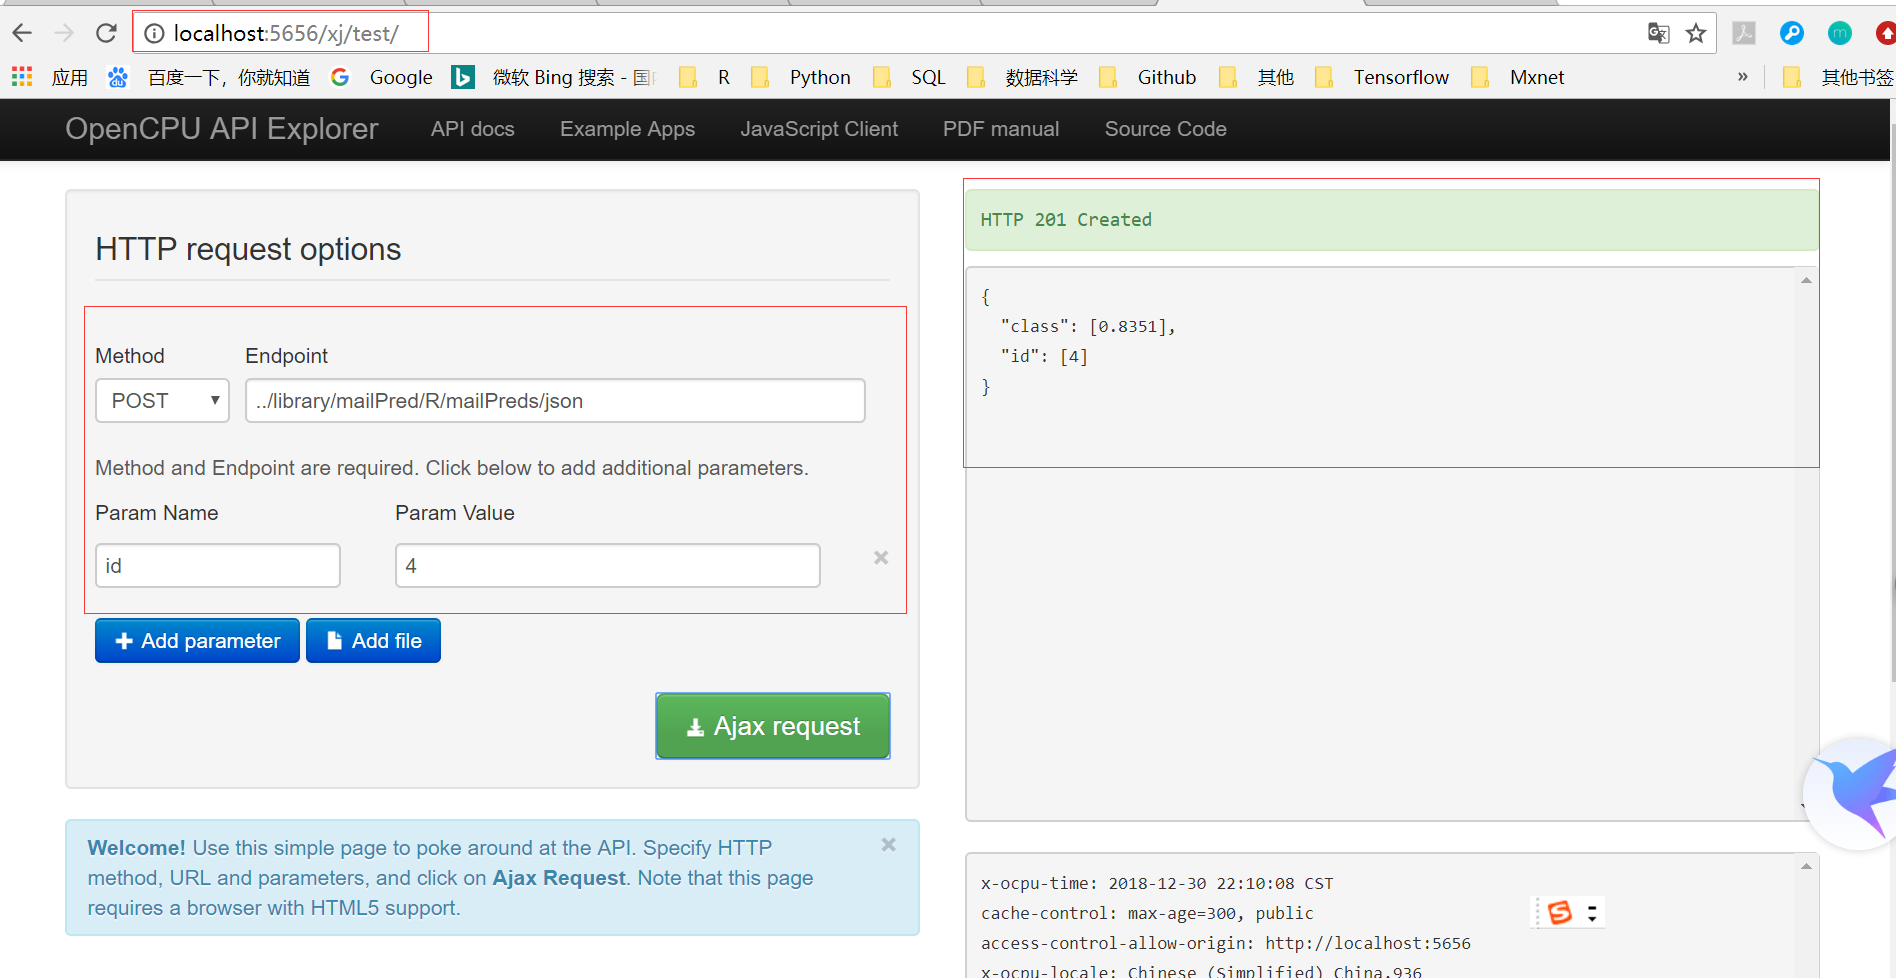
\includegraphics{pic/opencpu/p15.png}

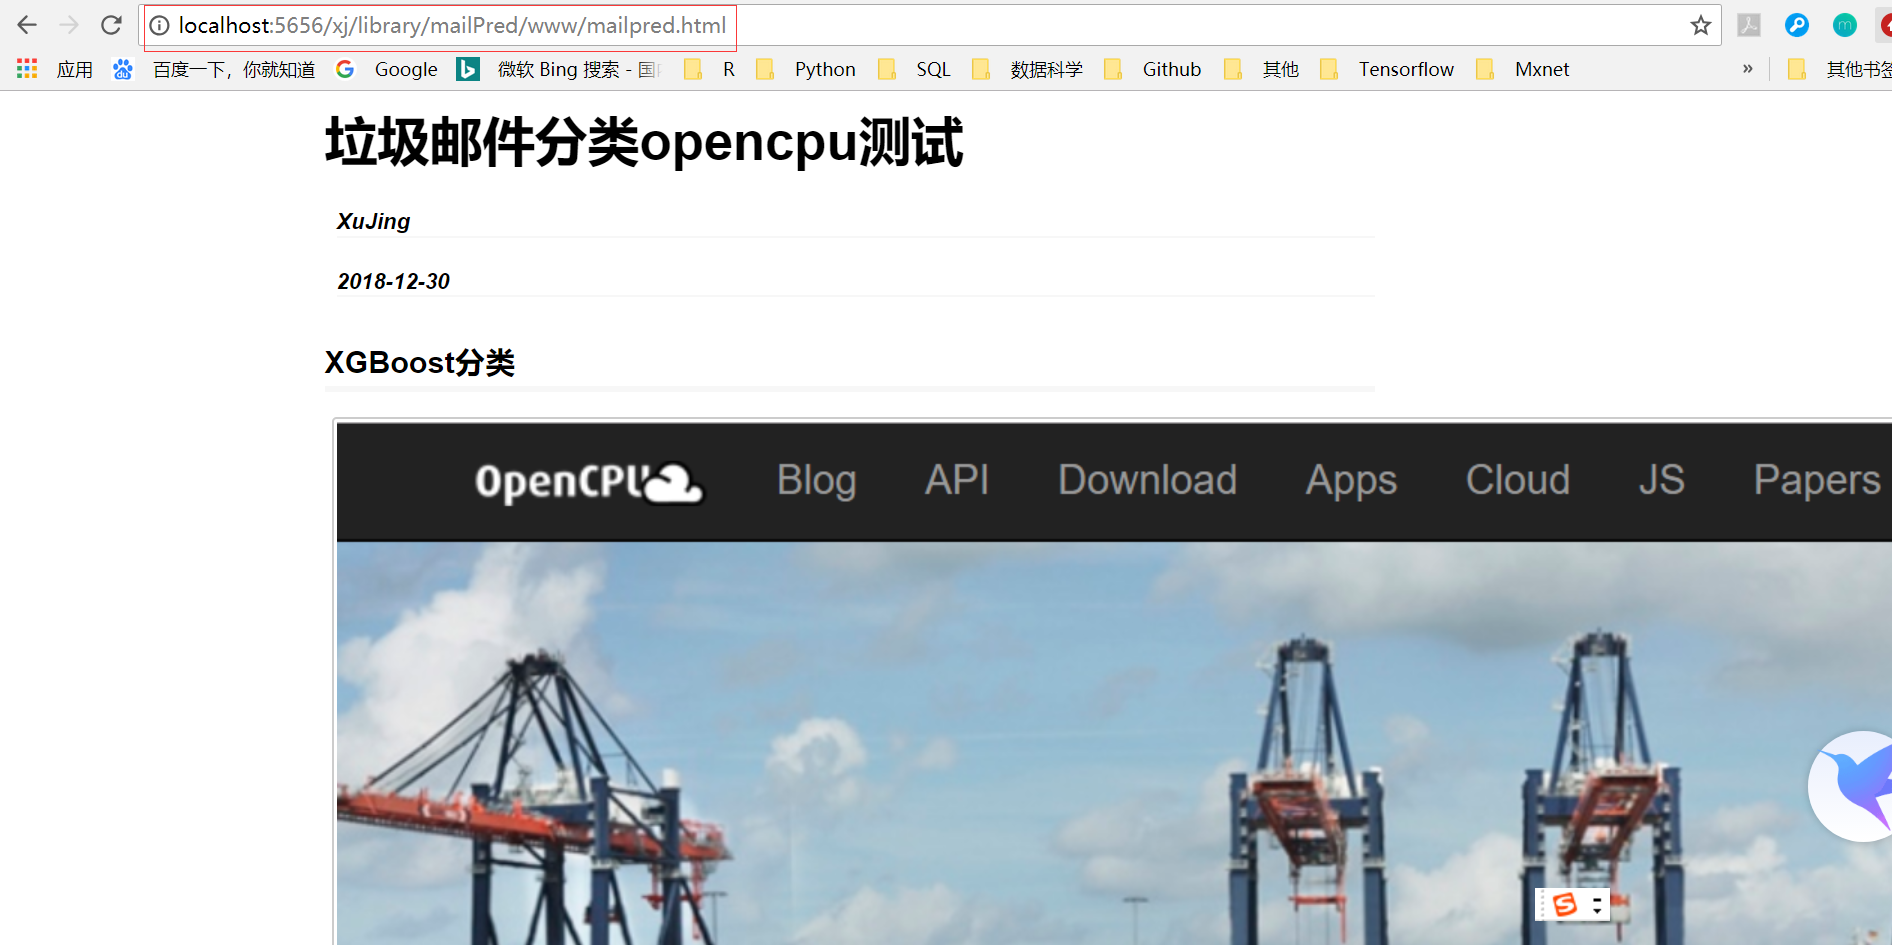
\includegraphics{pic/opencpu/p16.png}

\subsection{Ubuntu 16.04
opencpu-server部署测试}\label{ubuntu-16.04-opencpu-server}

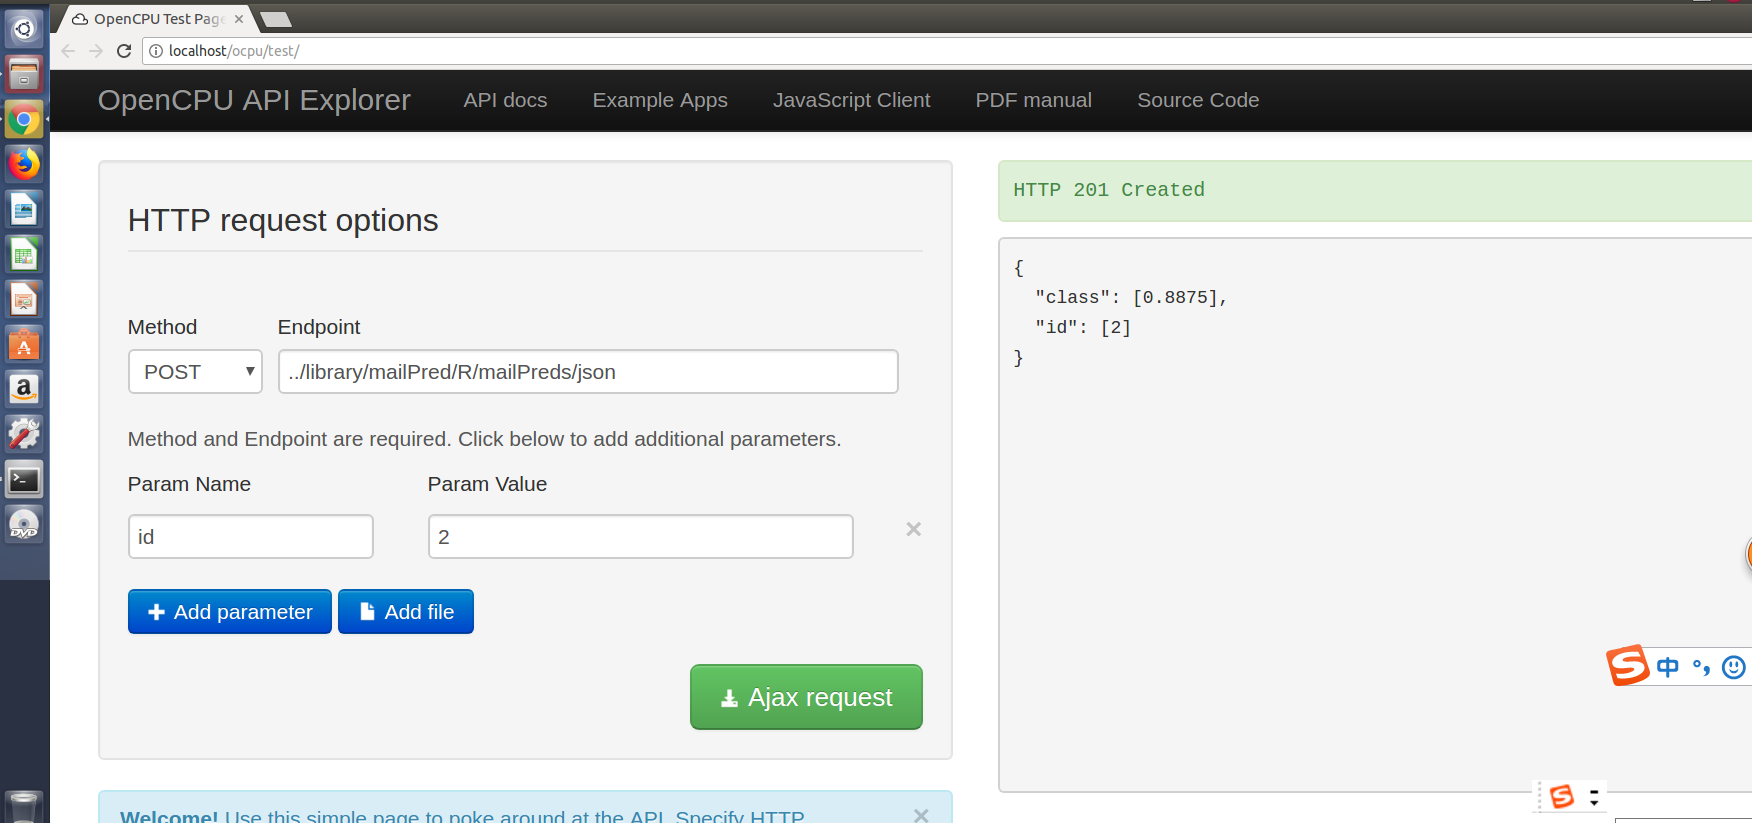
\includegraphics{pic/opencpu/p17.png}

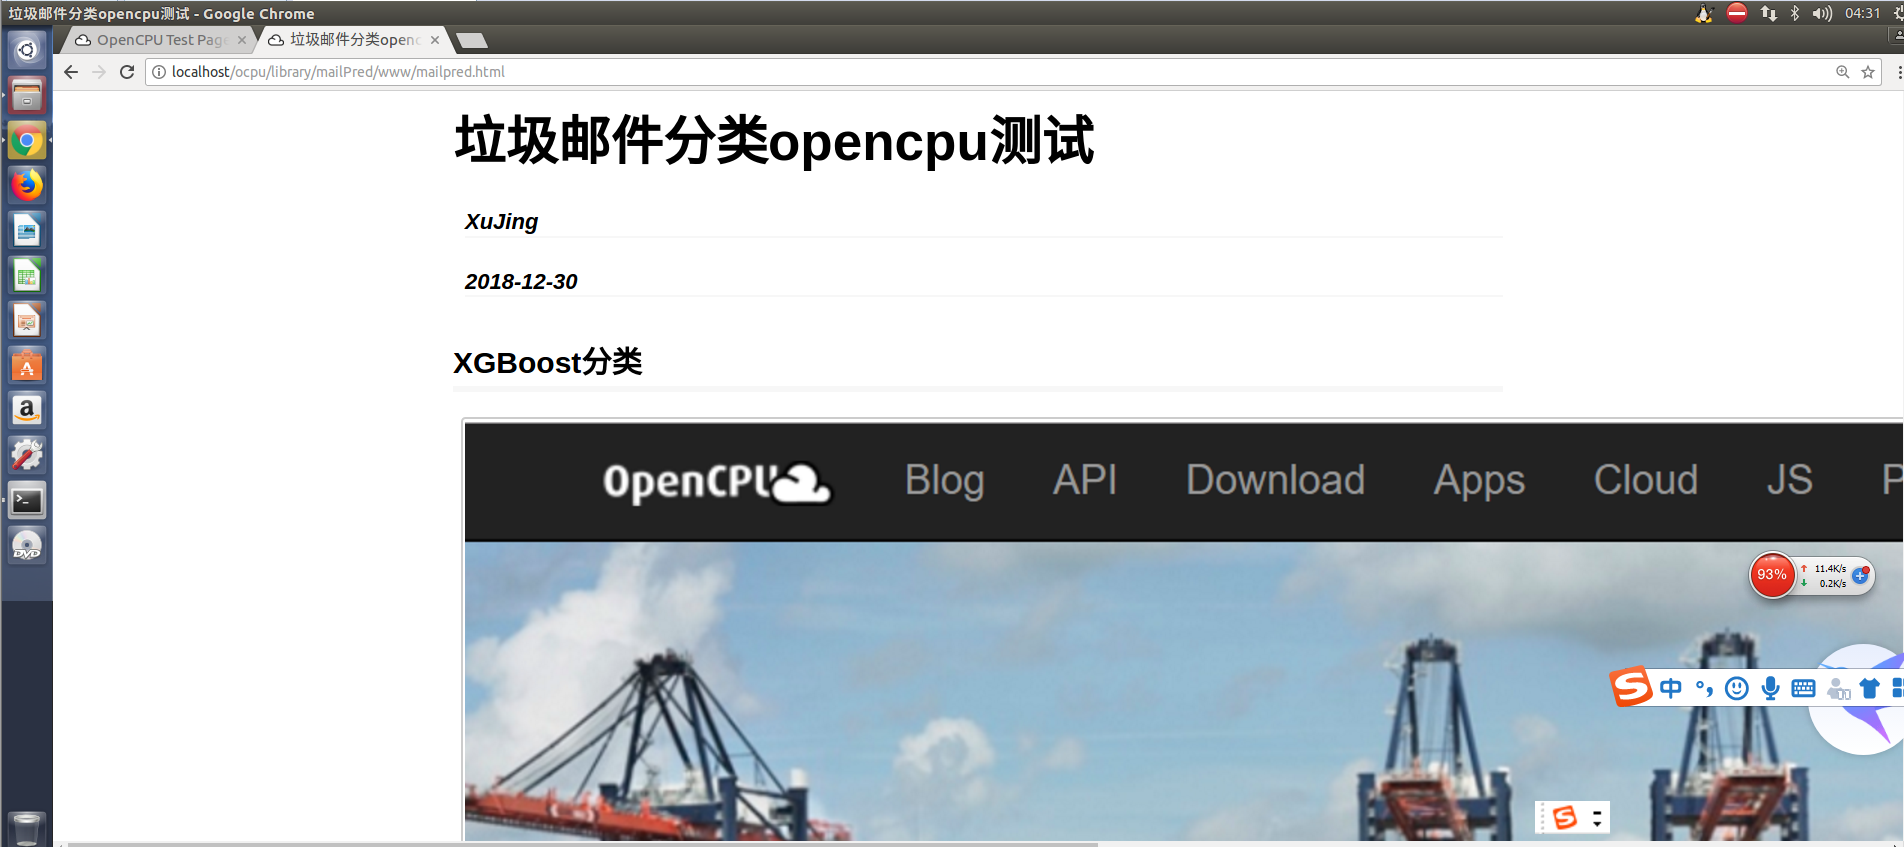
\includegraphics{pic/opencpu/p18.png}

\subsection{Github部署测试}\label{github}

详细的参考Github CI
Hook部分及\url{https://github.com/DataXujing/mailPred}

\subsection{官方例子}

官方提供了更多的例子,详细的可以参考\url{https://www.opencpu.org/apps.html}

\chapter{plumber}\label{plumber}


\includegraphics{pic/plumber/p2.png}

HTTP API已成为软件通信的主要语言。通过创建HTTP
API,您将使您的R代码能够被其他服务利用 -
无论它们是在您的组织内部还是托管在世界的另一端。以下是在您将R代码包装在Plumber
API中时向您打开的门的一些想法:

\begin{itemize}
\item
  在您的组织中使用其他语言编写的软件可以运行您的R代码。您公司的Java应用程序现在可以引入您按需生成的自定义ggplot2图表,或者Python客户端可以查询R中定义的预测模型。
\item
  您可以代表您使用某些\href{https://www.mailgun.com/}{第三方接收电子邮件},然后在新邮件到达时通知您的Plumber服务。
  您可以在Slack上注册一个``
  \href{https://api.slack.com/slash-commands}{Slash Command}
  '',使您能够执行R功能以响应Slack中输入的命令。
\item
  您可以编写从访问者的Web浏览器查询Plumber
  API的JavaScript代码。更进一步,您可以将Plumber专门用作交互式Web应用程序的后端。
\end{itemize}

Plumber托管在CRAN上,因此您可以通过运行以下命令下载并安装最新的稳定版本及其所有依赖项:

\begin{Shaded}
\begin{Highlighting}[]
\KeywordTok{install.paclages}\NormalTok{(}\StringTok{"plumber"}\NormalTok{)}
\end{Highlighting}
\end{Shaded}

或者,如果您想运行最新的不稳定开发版本plumber,可以使用该软件包从其GitHub存储库安装它devtools。

\begin{Shaded}
\begin{Highlighting}[]
\KeywordTok{install.packages}\NormalTok{(}\StringTok{"devtools"}\NormalTok{)}
\NormalTok{devtools}\OperatorTok{::}\KeywordTok{install_github}\NormalTok{(}\StringTok{"trestletech/plumber"}\NormalTok{)}
\end{Highlighting}
\end{Shaded}

\section{快速开始}

Plumber允许您通过仅使用特殊注释装饰现有R代码来创建API(\#*或\#')。下面的示例显示了一个名为plumber.R(Plumber
API的常规名称)的文件,该文件定义了API。

\begin{Shaded}
\begin{Highlighting}[]

\CommentTok{# plumber.R}

\CommentTok{#' Echo the parameter that was sent in}
\CommentTok{#' @param msg The message to echo back.}
\CommentTok{#' @get /echo}
\ControlFlowTok{function}\NormalTok{(}\DataTypeTok{msg=}\StringTok{""}\NormalTok{)\{}
  \KeywordTok{list}\NormalTok{(}\DataTypeTok{msg =} \KeywordTok{paste0}\NormalTok{(}\StringTok{"The message is: '"}\NormalTok{, msg, }\StringTok{"'"}\NormalTok{))}
\NormalTok{\}}


\CommentTok{#' Plot out data from the iris dataset}
\CommentTok{#' @param spec If provided, filter the data to only this species (e.g. 'setosa')}
\CommentTok{#' @get /plot}
\CommentTok{#' @png}
\ControlFlowTok{function}\NormalTok{(spec)\{}
\NormalTok{  myData <-}\StringTok{ }\NormalTok{iris}
\NormalTok{  title <-}\StringTok{ "All Species"}

  \CommentTok{# Filter if the species was specified}
  \ControlFlowTok{if}\NormalTok{ (}\OperatorTok{!}\KeywordTok{missing}\NormalTok{(spec))\{}
\NormalTok{    title <-}\StringTok{ }\KeywordTok{paste0}\NormalTok{(}\StringTok{"Only the '"}\NormalTok{, spec, }\StringTok{"' Species"}\NormalTok{)}
\NormalTok{    myData <-}\StringTok{ }\KeywordTok{subset}\NormalTok{(iris, Species }\OperatorTok{==}\StringTok{ }\NormalTok{spec)}
\NormalTok{  \}}

  \KeywordTok{plot}\NormalTok{(myData}\OperatorTok{$}\NormalTok{Sepal.Length, myData}\OperatorTok{$}\NormalTok{Petal.Length,}
       \DataTypeTok{main=}\NormalTok{title, }\DataTypeTok{xlab=}\StringTok{"Sepal Length"}\NormalTok{, }\DataTypeTok{ylab=}\StringTok{"Petal Length"}\NormalTok{)}
\NormalTok{\}}
\end{Highlighting}
\end{Shaded}

此文件定义了两个Plumber``端点''。一个托管在路径上/echo,只是回显传入的消息;
另一个托管在路径上/plot并返回一个显示简单R图的图像。

你可以使用plumber::plumb函数来此R档转换成管道工API:

\begin{Shaded}
\begin{Highlighting}[]
\NormalTok{pr <-}\StringTok{ }\NormalTok{plumber}\OperatorTok{::}\KeywordTok{plumb}\NormalTok{(}\StringTok{"plumber.R"}\NormalTok{)}
\end{Highlighting}
\end{Shaded}

该pr对象现在封装了plumber.R文件中表示的所有逻辑。下一步是使用以下run方法使API生效:

\begin{Shaded}
\begin{Highlighting}[]
\NormalTok{pr}\OperatorTok{$}\KeywordTok{run}\NormalTok{()}
\end{Highlighting}
\end{Shaded}

不妨运行试一下!!!

在前面的示例中,您看到了一个呈现为JSON的端点和一个生成图像的端点。除非另有说明,否则Plumber将尝试呈现您的端点函数返回的任何内容作为JSON。但是,您可以指定备用``序列化程序'',指示Plumber将输出呈现为其他格式,如HTML(\texttt{@html}),PNG(\texttt{@png})或JPEG(\texttt{@jpeg})

\begin{Shaded}
\begin{Highlighting}[]
\CommentTok{#' @get /hello}
\CommentTok{#' @html}
\ControlFlowTok{function}\NormalTok{()\{}
  \StringTok{"<html><h1>hello world</h1></html>"}
\NormalTok{\}}
\end{Highlighting}
\end{Shaded}

访问时,此端点将生成类似以下内容的内容。它还设置了适当的Content-Type标题,以便访问此页面的浏览器知道将结果呈现为HTML。

\begin{Shaded}
\begin{Highlighting}[]
\OperatorTok{<}\NormalTok{html}\OperatorTok{>}\ErrorTok{<}\NormalTok{h1}\OperatorTok{>}\NormalTok{hello world}\OperatorTok{<}\ErrorTok{/}\NormalTok{h1}\OperatorTok{>}\ErrorTok{</}\NormalTok{html}\OperatorTok{>}
\end{Highlighting}
\end{Shaded}

我们将在API的输出中详细讲解。

\section{路由和输入}

传入的HTTP请求必须``路由''到一个或多个R函数。Plumber有两个不同的函数系列:端点和过滤器。


\includegraphics{pic/plumber/p3.png}

通常,当请求到达Plumber路由器时,Plumber首先将该请求通过其过滤器。一旦所有过滤器处理了请求,路由器将查找可满足传入请求的端点。如果找到一个,它将调用端点并使用端点返回的值响应传入的请求。如果没有端点与请求匹配,则将404
Not Found返回错误(其行为可由set404Handler方法控制)详见自定义路由。

\subsection{端点}

此批注指定此函数负责生成对任何GET请求的响应/hello。从函数返回的值将用作对请求的响应(在通过序列化程序运行以将响应转换为JSON之后)。在这种情况下,GET响应/hello将返回{[}``hello
world''{]}带有的内容JSON Content-Type。

生成端点的注释包括:

\begin{itemize}
\item
  \texttt{@get}
\item
  \texttt{@post}
\item
  \texttt{@put}
\item
  \texttt{@delete}
\item
  \texttt{@head}
\end{itemize}

请注意,单个端点可以支持多个动词。下面的函数将被用来处理任何传入的GET,POST或PUT请求/cars

\begin{Shaded}
\begin{Highlighting}[]
\CommentTok{#' @get /cars}
\CommentTok{#' @post /cars}
\CommentTok{#' @put /cars}
\ControlFlowTok{function}\NormalTok{()\{}
\NormalTok{  ...}
\NormalTok{\}}
\end{Highlighting}
\end{Shaded}

\subsection{过滤器}

过滤器可用于定义用于处理传入请求的``管道''。这允许API作者将复杂的逻辑分解为一系列独立的,可理解的步骤。与端点不同,请求可以在生成响应之前通过多个Plumber过滤器。

通常,Plumber路由器会在尝试查找满足请求的端点之前,通过所有已定义的过滤器传递请求。

过滤器可以在处理请求时执行以下三种操作之一:

\begin{enumerate}
\def\labelenumi{\arabic{enumi}.}
\item
  可能在改变请求之后将控制转发到下一个处理程序。
\item
  返回响应本身而不是转发给后续处理程序
\item
  抛出一个错误
\end{enumerate}

\subsubsection{转发给另一个处理程序}

过滤器最常见的行为是在改变传入请求或调用某些外部副作用后将请求传递给下一个处理程序。一个常见的用例是使用过滤器作为请求记录器:

\begin{Shaded}
\begin{Highlighting}[]
\CommentTok{#* Log some information about the incoming request}
\CommentTok{#* @filter logger}
\ControlFlowTok{function}\NormalTok{(req)\{}
  \KeywordTok{cat}\NormalTok{(}\KeywordTok{as.character}\NormalTok{(}\KeywordTok{Sys.time}\NormalTok{()), }\StringTok{"-"}\NormalTok{, }
\NormalTok{    req}\OperatorTok{$}\NormalTok{REQUEST_METHOD, req}\OperatorTok{$}\NormalTok{PATH_INFO, }\StringTok{"-"}\NormalTok{, }
\NormalTok{    req}\OperatorTok{$}\NormalTok{HTTP_USER_AGENT, }\StringTok{"@"}\NormalTok{, req}\OperatorTok{$}\NormalTok{REMOTE_ADDR, }\StringTok{"}\CharTok{\textbackslash{}n}\StringTok{"}\NormalTok{)}
\NormalTok{  plumber}\OperatorTok{::}\KeywordTok{forward}\NormalTok{()}
\NormalTok{\}}
\end{Highlighting}
\end{Shaded}

此过滤器是直接的:它调用外部操作(日志记录),然后调用forward()将控制权传递给管道中的下一个处理程序(另一个过滤器或端点)

类似的过滤器可能会改变它给出的请求或响应对象上的某些状态

\begin{Shaded}
\begin{Highlighting}[]
\CommentTok{#* @filter setuser}
\ControlFlowTok{function}\NormalTok{(req)\{}
\NormalTok{  un <-}\StringTok{ }\NormalTok{req}\OperatorTok{$}\NormalTok{cookies}\OperatorTok{$}\NormalTok{user}
  \CommentTok{# Make req$username available to endpoints}
\NormalTok{  req}\OperatorTok{$}\NormalTok{username <-}\StringTok{ }\NormalTok{un}

\NormalTok{  plumber}\OperatorTok{::}\KeywordTok{forward}\NormalTok{()}
\NormalTok{\}}
\end{Highlighting}
\end{Shaded}

\subsubsection{返回响应}

过滤器也可以返回响应。您可能希望检查请求是否满足某些约束(如身份验证),并且
- 在某些情况下 -
返回响应而不调用任何其他处理程序。例如,可以使用过滤器来检查用户是否已经过身份验证。

\begin{Shaded}
\begin{Highlighting}[]
\CommentTok{#* @filter checkAuth}
\ControlFlowTok{function}\NormalTok{(req, res)\{}
  \ControlFlowTok{if}\NormalTok{ (}\KeywordTok{is.null}\NormalTok{(req}\OperatorTok{$}\NormalTok{username))\{}
\NormalTok{    res}\OperatorTok{$}\NormalTok{status <-}\StringTok{ }\DecValTok{401} \CommentTok{# Unauthorized}
    \KeywordTok{return}\NormalTok{(}\KeywordTok{list}\NormalTok{(}\DataTypeTok{error=}\StringTok{"Authentication required"}\NormalTok{))}
\NormalTok{  \} }\ControlFlowTok{else}\NormalTok{ \{}
\NormalTok{    plumber}\OperatorTok{::}\KeywordTok{forward}\NormalTok{()}
\NormalTok{  \}}
\NormalTok{\}}
\end{Highlighting}
\end{Shaded}

Plumber
API中出现错误的常见原因是忘记forward()在过滤器中调用。在这样的过滤器中,最后一行的结果将作为对传入请求的响应以静默方式返回。这可能会导致您的API表现出非常奇怪的行为,具体取决于返回的内容。当您使用过滤器时,请务必仔细审核所有代码路径,以确保您正在调用forward(),导致错误或故意返回值。

\subsubsection{抛出错误}

最后,过滤器可能会抛出错误。如果在定义过滤器的代码中出错或者过滤器故意调用stop()以触发错误,则会发生这种情况。在这种情况下,任何后续处理程序都不会处理请求,并且会立即将其发送到路由器的错误处理程序。有关如何自定义此错误处理程序的详细信息,请参阅路由器自定义。

\subsection{动态路由}

除了具有类似硬编码的路由之外/hello,Plumber端点还可以具有动态路由。动态路由允许端点定义一组更灵活的路径,以便它们匹配。

\begin{Shaded}
\begin{Highlighting}[]
\NormalTok{users <-}\StringTok{ }\KeywordTok{data.frame}\NormalTok{(}
  \DataTypeTok{uid=}\KeywordTok{c}\NormalTok{(}\DecValTok{12}\NormalTok{,}\DecValTok{13}\NormalTok{),}
  \DataTypeTok{username=}\KeywordTok{c}\NormalTok{(}\StringTok{"kim"}\NormalTok{, }\StringTok{"john"}\NormalTok{)}
\NormalTok{)}

\CommentTok{#' Lookup a user}
\CommentTok{#' @get /users/<id>}
\ControlFlowTok{function}\NormalTok{(id)\{}
  \KeywordTok{subset}\NormalTok{(users, uid}\OperatorTok{==}\NormalTok{id)}
\NormalTok{\}}
\end{Highlighting}
\end{Shaded}

此API使用动态路径/users/来匹配任何形式的请求,/users/后跟一些路径元素,如数字或字母。在这种情况下,如果找到具有相关ID的用户,则返回有关用户的信息,否则返回空对象。

此API使用动态路径/users/来匹配任何形式的请求,/users/后跟一些路径元素,如数字或字母。在这种情况下,如果找到具有相关ID的用户,则返回有关用户的信息,否则返回空对象。

您可以根据需要命名这些动态路径元素,但请注意,动态路径中使用的名称必须与函数的参数名称匹配(在本例中为两者id)。

您甚至可以执行更复杂的动态路由,例如:

\begin{Shaded}
\begin{Highlighting}[]
\CommentTok{#' @get /user/<from>/connect/<to>}
\ControlFlowTok{function}\NormalTok{(from, to)\{}
  \CommentTok{# Do something with the `from` and `to` variables...}
\NormalTok{\}}
\end{Highlighting}
\end{Shaded}

除非另有说明,否则从查询字符串或动态路径传递到管道工端点的所有参数都将是字符串。例如,请考虑以下API。

\begin{Shaded}
\begin{Highlighting}[]
\CommentTok{#' @get /type/<id>}
\ControlFlowTok{function}\NormalTok{(id)\{}
  \KeywordTok{list}\NormalTok{(}
    \DataTypeTok{id =}\NormalTok{ id,}
    \DataTypeTok{type =} \KeywordTok{typeof}\NormalTok{(id)}
\NormalTok{  )}
\NormalTok{\}}
\end{Highlighting}
\end{Shaded}

访问http:// localhost:8000 / types / 14将返回:

\begin{Shaded}
\begin{Highlighting}[]
\NormalTok{\{}
  \StringTok{"id"}\OperatorTok{:}\StringTok{ }\NormalTok{[}\StringTok{"14"}\NormalTok{],}
  \StringTok{"type"}\OperatorTok{:}\StringTok{ }\NormalTok{[}\StringTok{"character"}\NormalTok{]}
\NormalTok{\}}
\end{Highlighting}
\end{Shaded}

如果您只打算支持动态路由中特定参数的特定数据类型,则可以在路径本身中指定所需的类型。

\begin{Shaded}
\begin{Highlighting}[]
\CommentTok{#* @get /user/<id:int>}
\ControlFlowTok{function}\NormalTok{(id)\{}
  \ControlFlowTok{next}\NormalTok{ <-}\StringTok{ }\NormalTok{id }\OperatorTok{+}\StringTok{ }\DecValTok{1}
  \CommentTok{# ...}
\NormalTok{\}}

\CommentTok{#* @post /user/activated/<active:bool>}
\ControlFlowTok{function}\NormalTok{(active)\{}
  \ControlFlowTok{if}\NormalTok{ (}\OperatorTok{!}\NormalTok{active)\{}
    \CommentTok{# ...}
\NormalTok{  \}}
\NormalTok{\}}
\end{Highlighting}
\end{Shaded}

下面详细介绍了可以在动态类型中使用的类型名称的映射以及它们如何映射到R数据类型。

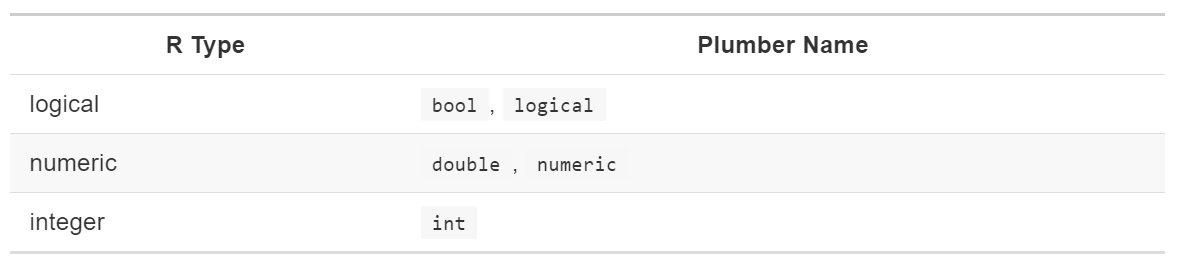
\includegraphics{pic/plumber/p4.png}

\subsubsection{静态文件处理}

plumber包括一个静态文件服务器,可用于托管静态资源(如JavaScript,CSS或HTML文件)的目录。这些服务器配置相当简单,并且可以集成到plumber应用程序中。

\begin{Shaded}
\begin{Highlighting}[]
\CommentTok{#* @assets ./files/static}
\KeywordTok{list}\NormalTok{()}
\end{Highlighting}
\end{Shaded}

此示例将在服务器./files/static的默认/public路径中公开本地目录。因此,如果您有一个文件./files/static/branding.html,它将在您的plumber服务器上可用/public/branding.html。

您可以选择提供其他参数来配置用于服务器的公共路径。例如

\begin{Shaded}
\begin{Highlighting}[]
\CommentTok{#* @assets ./files/static /static}
\KeywordTok{list}\NormalTok{()}
\end{Highlighting}
\end{Shaded}

请求的目录不在/public,但在/static

在上面的示例中,服务器的``实现''只是一个空的list()。还可以指定function()与其他plumber注释类似的操作。此时,实现不会改变静态服务器的行为。最终,此列表或函数可以通过更改缓存控制设置等内容来提供配置服务器的机会。

\subsubsection{输入处理}

根据传入HTTP请求的路径和方法路由请求,但请求可以包含比此更多的信息。它们可能包含其他HTTP标头,查询字符串或请求正文。所有这些字段都可以被视为您的Plumber
API的``输入''。

这个可以详细的参考plumber的官方文档,在此不再赘述。

\section{Rendering Output}\label{rendering-output}

\subsection{序列化器}

默认情况下,Plumber通过jsonliteR包将对象序列化为JSON
。但是,包中内置了各种其他序列化程序。

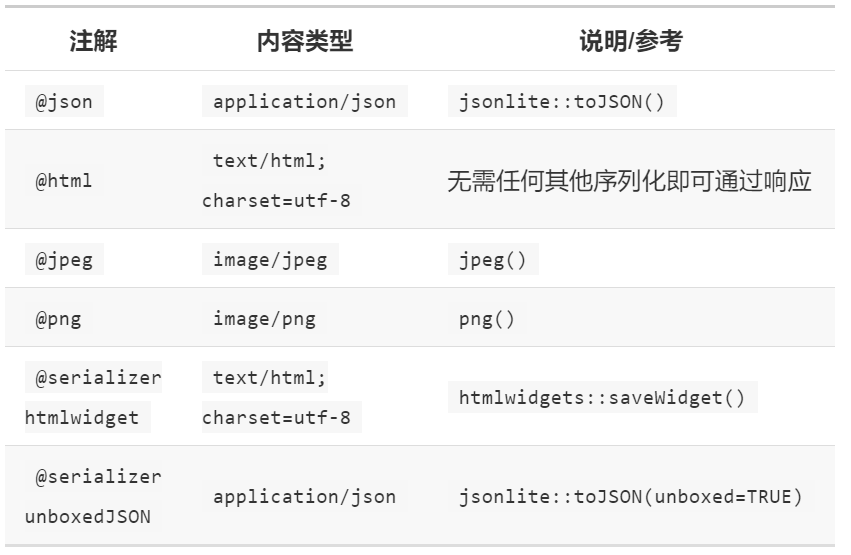
\includegraphics{pic/plumber/p5.png}

\subsection{绕过序列化}

在某些情况下,可能需要直接从R返回值而不进行序列化。您可以通过从端点返回响应对象来绕过序列化。例如,请考虑以下API

\begin{Shaded}
\begin{Highlighting}[]
\CommentTok{#' Endpoint that bypasses serialization}
\CommentTok{#' @get /}
\ControlFlowTok{function}\NormalTok{(res)\{}
\NormalTok{  res}\OperatorTok{$}\NormalTok{body <-}\StringTok{ "Literal text here!"}

\NormalTok{  res}
\NormalTok{\}}
\end{Highlighting}
\end{Shaded}

从此端点返回的响应将包含Literal text
here!没有Content-Type标头且没有任何其他序列化的主体。

同样,您可以利用\texttt{@serializer\ contentType}不对响应进行序列化但指定contentType标头的注释。如果希望更好地控制发送的响应,可以使用此批注。

\begin{Shaded}
\begin{Highlighting}[]
\CommentTok{#* @serializer contentType list(type="application/pdf")}
\CommentTok{#* @get /pdf}
\ControlFlowTok{function}\NormalTok{()\{}
\NormalTok{  tmp <-}\StringTok{ }\KeywordTok{tempfile}\NormalTok{()}
  \KeywordTok{pdf}\NormalTok{(tmp)}
  \KeywordTok{plot}\NormalTok{(}\DecValTok{1}\OperatorTok{:}\DecValTok{10}\NormalTok{, }\DataTypeTok{type=}\StringTok{"b"}\NormalTok{)}
  \KeywordTok{text}\NormalTok{(}\DecValTok{4}\NormalTok{, }\DecValTok{8}\NormalTok{, }\StringTok{"PDF from plumber!"}\NormalTok{)}
  \KeywordTok{text}\NormalTok{(}\DecValTok{6}\NormalTok{, }\DecValTok{2}\NormalTok{, }\KeywordTok{paste}\NormalTok{(}\StringTok{"The time is"}\NormalTok{, }\KeywordTok{Sys.time}\NormalTok{()))}
  \KeywordTok{dev.off}\NormalTok{()}

  \KeywordTok{readBin}\NormalTok{(tmp, }\StringTok{"raw"}\NormalTok{, }\DataTypeTok{n=}\KeywordTok{file.info}\NormalTok{(tmp)}\OperatorTok{$}\NormalTok{size)}
\NormalTok{\}}
\end{Highlighting}
\end{Shaded}

运行此API并访问http://localhost:8000/pdf将下载从R生成的PDF(如果您的客户支持,则本机显示PDF)

\subsection{boxed and unboxed JSON}\label{boxed-and-unboxed-json}

您可能已经注意到,从Plumber生成的API响应将奇异值(或``标量'')呈现为数组。例如:

\begin{Shaded}
\begin{Highlighting}[]
\NormalTok{jsonlite}\OperatorTok{::}\KeywordTok{toJSON}\NormalTok{(}\KeywordTok{list}\NormalTok{(}\DataTypeTok{a=}\DecValTok{5}\NormalTok{))}
\end{Highlighting}
\end{Shaded}

\begin{verbatim}
## {"a":[5]}
\end{verbatim}

a元素的值虽然是单数,但仍然呈现为数组。这可能会让您感到惊讶,但这样做是为了保持输出的一致性。虽然JSON将标量与矢量对象区分开来,但R却没有。这在将R对象序列化为JSON时会产生歧义,因为不清楚特定元素是应该呈现为原子值还是JSON数组。

考虑以下API,它以字典方式返回比给定字母``更高''的所有字母。

\begin{Shaded}
\begin{Highlighting}[]
\CommentTok{#' Get letters after a given letter}
\CommentTok{#' @get /boxed}
\ControlFlowTok{function}\NormalTok{(}\DataTypeTok{letter=}\StringTok{"A"}\NormalTok{)\{}
\NormalTok{  LETTERS[LETTERS }\OperatorTok{>}\StringTok{ }\NormalTok{letter]}
\NormalTok{\}}

\CommentTok{#' Get letters after a given letter}
\CommentTok{#' @serializer unboxedJSON}
\CommentTok{#' @get /unboxed}
\ControlFlowTok{function}\NormalTok{(}\DataTypeTok{letter=}\StringTok{"A"}\NormalTok{)\{}
\NormalTok{  LETTERS[LETTERS }\OperatorTok{>}\StringTok{ }\NormalTok{letter]}
\NormalTok{\}}
\end{Highlighting}
\end{Shaded}

访问http:// localhost:8000 / boxed?letter = U或http://
localhost:8000 / unboxed?letter = U将返回相同的响应

\begin{Shaded}
\begin{Highlighting}[]
\NormalTok{[}\StringTok{"V"}\NormalTok{, }\StringTok{"W"}\NormalTok{, }\StringTok{"X"}\NormalTok{, }\StringTok{"Y"}\NormalTok{, }\StringTok{"Z"}\NormalTok{]}
\end{Highlighting}
\end{Shaded}

但是,http:// localhost:8000 / boxed?letter = Y将产生:

\begin{Shaded}
\begin{Highlighting}[]
\NormalTok{[}\StringTok{"Z"}\NormalTok{]}
\end{Highlighting}
\end{Shaded}

而http:// localhost:8000 / unboxed?letter = Y将产生:

\begin{Shaded}
\begin{Highlighting}[]
\StringTok{"Z"}
\end{Highlighting}
\end{Shaded}

Plumber继承了jsonlite::toJSON设置的默认值,auto\_unbox=FALSE这将导致所有长度为1的向量仍然呈现为JSON数组。unboxedJSON如果要更改特定端点的此行为,可以将端点配置为使用序列化程序(如上所示)

\subsection{自定义图像序列化程序}

\texttt{@jpeg}和\texttt{@png}分别返回到客户端jpeg()或png()功能。这些功能接受各种各样的定制包括输出额外的选项width,height以及bg等等

\begin{Shaded}
\begin{Highlighting}[]
\CommentTok{#' Example of customizing graphical output}
\CommentTok{#' @png (width = 400, height = 500)}
\CommentTok{#' @get /}
\ControlFlowTok{function}\NormalTok{()\{}
  \KeywordTok{plot}\NormalTok{(}\DecValTok{1}\OperatorTok{:}\DecValTok{10}\NormalTok{)}
\NormalTok{\}}
\end{Highlighting}
\end{Shaded}

\subsection{错误处理}

Plumber包装每个端点调用,以便它可以正常捕获错误。

\begin{Shaded}
\begin{Highlighting}[]
\CommentTok{#' Example of throwing an error}
\CommentTok{#' @get /simple}
\ControlFlowTok{function}\NormalTok{()\{}
  \KeywordTok{stop}\NormalTok{(}\StringTok{"I'm an error!"}\NormalTok{) }\CommentTok{# 状态代码为500}
\NormalTok{\}}

\CommentTok{#' Generate a friendly error}
\CommentTok{#' @get /friendly}
\ControlFlowTok{function}\NormalTok{(res)\{}
\NormalTok{  msg <-}\StringTok{ "Your request did not include a required parameter."}
\NormalTok{  res}\OperatorTok{$}\NormalTok{status <-}\StringTok{ }\DecValTok{400} \CommentTok{# Bad request}
  \KeywordTok{list}\NormalTok{(}\DataTypeTok{error=}\NormalTok{jsonlite}\OperatorTok{::}\KeywordTok{unbox}\NormalTok{(msg))}
\NormalTok{\}}
\end{Highlighting}
\end{Shaded}

\subsection{设置Cookies(*)}\label{cookies}

作为完成请求的一部分,Plumber API可以选择在客户端上设置HTTP cookie。HTTP
API不会隐式包含``会话''的概念。如果没有一些附加信息,Plumber无法确定进来的两个HTTP请求是否与同一用户相关联。Cookie提供了一种方法来委托客户端代表您存储某些状态,以便所选数据可以比单个HTTP请求更长时间;
这里讨论使用cookie跟踪API中的状态的全部含义。

\subsubsection{设置未加密的Cookie}\label{cookie}

下面的API端点将返回一个随机字母,但它会记住您是否喜欢大写或小写字母的首选项。

\begin{Shaded}
\begin{Highlighting}[]
\CommentTok{#' @put /preferences}
\ControlFlowTok{function}\NormalTok{(res, capital)\{}
  \ControlFlowTok{if}\NormalTok{ (}\KeywordTok{missing}\NormalTok{(capital))\{}
    \KeywordTok{stop}\NormalTok{(}\StringTok{"You must specify a value for the 'capital' preference."}\NormalTok{)}
\NormalTok{  \}}
\NormalTok{  res}\OperatorTok{$}\KeywordTok{setCookie}\NormalTok{(}\StringTok{"capitalize"}\NormalTok{, capital)}
\NormalTok{\}}

\CommentTok{#' @get /letter}
\ControlFlowTok{function}\NormalTok{(req) \{}
\NormalTok{  capitalize <-}\StringTok{ }\NormalTok{req}\OperatorTok{$}\NormalTok{cookies}\OperatorTok{$}\NormalTok{capitalize}

  \CommentTok{# Default to lower-case unless user preference is capitalized}
\NormalTok{  alphabet <-}\StringTok{ }\NormalTok{letters}

  \CommentTok{# The capitalize cookie will initially be empty (NULL)}
  \ControlFlowTok{if}\NormalTok{ (}\OperatorTok{!}\KeywordTok{is.null}\NormalTok{(capitalize) }\OperatorTok{&&}\StringTok{ }\NormalTok{capitalize }\OperatorTok{==}\StringTok{ "1"}\NormalTok{)\{}
\NormalTok{    alphabet <-}\StringTok{ }\NormalTok{LETTERS}
\NormalTok{  \}}

  \KeywordTok{list}\NormalTok{(}
    \DataTypeTok{letter =} \KeywordTok{sample}\NormalTok{(alphabet, }\DecValTok{1}\NormalTok{)}
\NormalTok{  )}
\NormalTok{\}}
\end{Highlighting}
\end{Shaded}

由于此API使用PUT请求来测试此API,因此我们将curl在命令行上使用它来测试它。(没有任何关于需要PUT请求的cookie
;您可以轻松地修改此API以使用GET请求。)我们可以从访问/letter端点开始,我们将看到API默认为小写字母。curl
\url{http://localhost:8000/letter}

\begin{Shaded}
\begin{Highlighting}[]
\NormalTok{\{}
  \StringTok{"letter"}\OperatorTok{:}\StringTok{ }\NormalTok{[}\StringTok{"y"}\NormalTok{]}
\NormalTok{\}}
\end{Highlighting}
\end{Shaded}

如果我们发送PUT请求并指定capital参数,则将在客户端上设置cookie,以允许服务器在将来的请求中容纳我们的首选项。在curl,您需要使用该-c选项指定要在其中保存这些cookie的文件。这是一个很好的提醒,客户端处理cookie的方式不同
- 有些人根本不会支持它们 -
所以如果你想使用它们,请确保你打算用API支持的客户端很好地使用cookie。

要发送PUT请求,将参数设置capital为1,我们可以调用:curl -c cookies.txt
-X PUT --data `capital=1'
``\url{http://localhost:8000/preferences}''。如果您打印出该cookies.txt文件,您现在应该看到它包含一个名为capitalize值的cookie
1。

我们可以提出另一个GET请求,/letter看它是否符合我们的偏好。但是我们需要告诉curl我们使用-b交换机发送此请求时使用我们刚刚创建的cookie文件:curl
-b cookies.txt
\url{http://localhost:8000/letter。您现在应该看到API返回一个随机的大写字母}。

\subsubsection{设置加密的cookie}\label{cookie}

除了存储纯文本cookie之外,Plumber还支持处理加密的cookie,加密的cookie会阻止用户查看其中存储的内容,并对其内容进行签名,以便用户无法修改存储的内容。

要使用此功能,必须在构建路由器后将其明确添加到路由器中。例如,您可以运行以下命令序列来创建支持加密会话cookie的路由器。

\begin{Shaded}
\begin{Highlighting}[]
\NormalTok{pr <-}\StringTok{ }\KeywordTok{plumb}\NormalTok{(}\StringTok{"myfile.R"}\NormalTok{)}
\NormalTok{pr}\OperatorTok{$}\KeywordTok{registerHooks}\NormalTok{(}\KeywordTok{sessionCookie}\NormalTok{(}\StringTok{"mySecretHere"}\NormalTok{, }\StringTok{"cookieName"}\NormalTok{))}
\NormalTok{pr}\OperatorTok{$}\KeywordTok{run}\NormalTok{()}
\end{Highlighting}
\end{Shaded}

你会注意到上面的例子正在使用sessionCookiePlumber附带的钩子。通过在路由器上添加注册这些挂钩,您将确保该req\$session对象在传入请求中可用,并且cookieName在响应准备好发送给用户时持久保存到命名的cookie
。在这个例子中,用于加密数据的密钥``mySecretHere''显然是一个非常弱的密钥。

与之不同的是\texttt{res\$setHeader()},附加的值\texttt{req\$session}
是通过序列化的jsonlite;
这样您就可以自由地在会话中使用更复杂的数据结构,例如列表。与此不同的是\texttt{res\$setHeaders()},\texttt{req\$session}使用您提供的密钥作为sessionCookie()函数的第一个参数来加密数据。

例如,我们将存储一个加密的cookie,用于计算此客户端访问特定端点的次数:

\begin{Shaded}
\begin{Highlighting}[]
\CommentTok{#* @get /sessionCounter}
\ControlFlowTok{function}\NormalTok{(req)\{}
\NormalTok{  count <-}\StringTok{ }\DecValTok{0}
  \ControlFlowTok{if}\NormalTok{ (}\OperatorTok{!}\KeywordTok{is.null}\NormalTok{(req}\OperatorTok{$}\NormalTok{session}\OperatorTok{$}\NormalTok{counter))\{}
\NormalTok{    count <-}\StringTok{ }\KeywordTok{as.numeric}\NormalTok{(req}\OperatorTok{$}\NormalTok{session}\OperatorTok{$}\NormalTok{counter)}
\NormalTok{  \}}
\NormalTok{  req}\OperatorTok{$}\NormalTok{session}\OperatorTok{$}\NormalTok{counter <-}\StringTok{ }\NormalTok{count }\OperatorTok{+}\StringTok{ }\DecValTok{1}
  \KeywordTok{return}\NormalTok{(}\KeywordTok{paste0}\NormalTok{(}\StringTok{"This is visit #"}\NormalTok{, count))}
\NormalTok{\}}
\end{Highlighting}
\end{Shaded}

同样,sessionCookie()在此代码工作之前,您需要在路由器上注册挂钩。

如果您检查浏览器中设置的cookie,您会发现它的值在到达客户端时已加密。但是当它到达Plumber时,您的cookie可以作为常规R列表使用,并且可以被读取或修改。

\section{部署}

不要使用run()方法,部署自己的API,这样是很危险的!对于plumber的生产环境的部署有如下方式:
DigitalOcean,RStudio Connect,Docker, pm2。在这里我们着重介绍plumber
API部署在Docker和pm2,
我们将举一个具体的时机例子并测试我们生产环境的部署效果。

\subsection{Docker(基础)}\label{docker}

在此不会深入研究Docker的细节或如何在系统上设置或安装所有内容。Docker
为那些希望入门的人提供了一些\href{https://docs.docker.com/}{很好的资源}。在这里,我们假设您已安装Docker,并且您熟悉启动容器所需的基本命令。

\href{https://hub.docker.com/r/trestletech/plumber/}{安装镜像}

\begin{Shaded}
\begin{Highlighting}[]
\NormalTok{docker pull trestletech}\OperatorTok{/}\NormalTok{plumber}

\CommentTok{#查看现在系统中存在的镜像}
\NormalTok{docker images }

\CommentTok{# 后边会常用的docker命令}
\NormalTok{docker pull }\OperatorTok{**}
\NormalTok{docker ps }\CommentTok{# 查看正在运行的容器列表}
\NormalTok{docker stop IDs}
\NormalTok{docker rmi IDs}
\NormalTok{docker rm XXX}
\end{Highlighting}
\end{Shaded}

运行服务

\begin{Shaded}
\begin{Highlighting}[]
\NormalTok{docker run }\OperatorTok{--}\NormalTok{rm }\OperatorTok{-}\NormalTok{p }\DecValTok{8000}\OperatorTok{:}\DecValTok{8000}\NormalTok{ trestletech}\OperatorTok{/}\NormalTok{plumber \textbackslash{}}
  \OperatorTok{/}\NormalTok{usr}\OperatorTok{/}\NormalTok{local}\OperatorTok{/}\NormalTok{lib}\OperatorTok{/}\NormalTok{R}\OperatorTok{/}\NormalTok{site}\OperatorTok{-}\NormalTok{library}\OperatorTok{/}\NormalTok{plumber}\OperatorTok{/}\NormalTok{examples}\OperatorTok{/}\DecValTok{04}\OperatorTok{-}\NormalTok{mean}\OperatorTok{-}\NormalTok{sum}\OperatorTok{/}\NormalTok{plumber.R}
\end{Highlighting}
\end{Shaded}

\begin{itemize}
\item
  \texttt{docker\ run} 告诉Docker运行一个新容器
\item
  \texttt{-\/-rm} 告诉Docker在容器完成后进行清理
\item
  \texttt{-p\ 8000:8000}
  说将端口8000从plumber容器(我们将运行服务器的位置)映射到本地计算机的端口8000
\item
  \texttt{trestletech/plumber} 是我们要运行的镜像的名称
\item
  \texttt{/usr/local/lib/R/site-library/plumber/examples/03-mean-sum/plumber.R}是Docker容器内部到您要托管的Plumber文件的路径。
\end{itemize}

\begin{Shaded}
\begin{Highlighting}[]
\NormalTok{docker run }\OperatorTok{--}\NormalTok{rm }\OperatorTok{-}\NormalTok{p }\DecValTok{8000}\OperatorTok{:}\DecValTok{8000} \OperatorTok{-}\NormalTok{v }\StringTok{`}\DataTypeTok{pwd}\StringTok{`}\OperatorTok{/}\NormalTok{api.R}\OperatorTok{:}\ErrorTok{/}\NormalTok{plumber.R trestletech}\OperatorTok{/}\NormalTok{plumber }\OperatorTok{/}\NormalTok{plumber.R}
\end{Highlighting}
\end{Shaded}

\begin{itemize}
\tightlist
\item
  \texttt{-v} 把当前工作目录下的api.R 挂载到镜像中的/plumber.R的目录下
\item
  定义了该文件的位置应为/plumber.R,所以我们最后给出的参数告诉容器在哪里查找plumber定义
\end{itemize}

\subsection{Docker(高级)}\label{docker}

关于多plumber部署,同一端口的多应用部署,负载均衡,可以参考\url{https://www.rplumber.io/docs/hosting.html\#custom-dockerfiles}

\subsection{pm2}\label{pm2}

不熟悉在Docker中托管API
,那么您需要找到一种运行方式,直接管理服务器上的Plumber API。

pm2是一个最初以Node.js为目标的流程管理器。这里我们将展示在Ubuntu
14.04中执行此操作所需的命令,但您可以使用pm2支持的任何操作系统或分发。最后,您将拥有一台服务器,可在启动时自动启动plumber服务,如果它们崩溃则重新启动它们,甚至可以集中管理管道服务的日志。

\subsubsection{安装pm2}\label{pm2}

现在您已准备好安装pm2。pm2是npm(Node.js的包管理系统)中维护的包;
它还需要Node.js才能运行。所以要开始你要安装Node.js. 在Ubuntu
14.04上,必要的命令是:

\begin{Shaded}
\begin{Highlighting}[]
\NormalTok{sudo apt}\OperatorTok{-}\NormalTok{get update}
\NormalTok{sudo apt}\OperatorTok{-}\NormalTok{get install nodejs npm}
\CommentTok{# 由于Ubuntu下已经有一个名叫node的库,因此Node.js在ubuntu下默认叫nodejs,需要额外处理一下}
\NormalTok{sudo ln }\OperatorTok{-}\NormalTok{s }\OperatorTok{/}\NormalTok{usr}\OperatorTok{/}\NormalTok{bin}\OperatorTok{/}\NormalTok{nodejs }\OperatorTok{/}\NormalTok{usr}\OperatorTok{/}\NormalTok{bin}\OperatorTok{/}\NormalTok{node}
\end{Highlighting}
\end{Shaded}

一旦安装了npm和Node.js,就可以安装pm2了。

\begin{Shaded}
\begin{Highlighting}[]
\NormalTok{sudo npm install }\OperatorTok{-}\NormalTok{g pm2}
\end{Highlighting}
\end{Shaded}

这将-g在您的服务器上安装pm2 global(),这意味着您现在应该能够运行pm2
--version并获取已安装的pm2的版本号。

为了让pm2在启动时启动你的服务,你应该运行sudo pm2
startup它将为你的系统创建必要的文件,以便在你启动你的机器时运行pm2。

\subsubsection{Wrap Your Plumber File}\label{wrap-your-plumber-file}

将Plumber文件部署到服务器后,您仍需要告诉服务器如何运行服务器。你可能习惯于运行像这样的命令

\begin{Shaded}
\begin{Highlighting}[]
\NormalTok{pr <-}\StringTok{ }\KeywordTok{plumb}\NormalTok{(}\StringTok{"myfile.R"}\NormalTok{)}
\NormalTok{pr}\OperatorTok{$}\KeywordTok{run}\NormalTok{(}\DataTypeTok{port=}\DecValTok{4500}\NormalTok{)}
\end{Highlighting}
\end{Shaded}

不幸的是,pm2本身并不理解R脚本; 您可以使用该pm2
list命令查看pm2已在运行的服务。如果您现在运行此命令,您将看到pm2没有任何它负责的服务。将脚本和代码存储在所需目录中后,使用以下命令告知pm2您的服务。

\begin{Shaded}
\begin{Highlighting}[]
\NormalTok{pm2 start }\OperatorTok{--}\NormalTok{interpreter=}\StringTok{"Rscript"} \OperatorTok{/}\NormalTok{usr}\OperatorTok{/}\NormalTok{local}\OperatorTok{/}\NormalTok{plumber}\OperatorTok{/}\NormalTok{myfile}\OperatorTok{/}\NormalTok{run}\OperatorTok{-}\NormalTok{myfile.R}
\end{Highlighting}
\end{Shaded}

您应该看到有关pm2的一些输出,它们启动了您的服务实例,然后是pm2的一些状态信息。如果一切正常,您将看到您的新服务已注册并正在运行。您可以通过pm2
list再次执行来查看相同的输出。

一旦您对已定义的pm2服务感到满意,您可以使用pm2
save告诉pm2保留下次启动计算机时运行的服务集。您定义的所有服务都将自动重新启动。

\begin{itemize}
\tightlist
\item
  如果要查看更多信息,使用\texttt{pm2\ show\ run-myfile}
\item
  如果您需要检查服务的日志文件,则可以运行\texttt{pm2\ logs\ run-myfile}
\item
  如果您想要查看服务器和所有pm2服务的运行状况的大图,您可以运行pm2
  monit它将显示所有服务的RAM和CPU使用情况的仪表板。
\end{itemize}

\subsection{XGBoost模型预测部署实例}\label{xgboost}

我们将给予XGBoost模型,通过一个具体的实例演示从模型的训练到部署的整个过程,这里我们分别采用docker和pm2部署我们的模型

\begin{itemize}
\tightlist
\item
  1.模型的训练与预测
\end{itemize}

\begin{Shaded}
\begin{Highlighting}[]
\CommentTok{# 垃圾邮件分类,一共57个特征}
\KeywordTok{library}\NormalTok{(xgboost)}
\KeywordTok{library}\NormalTok{(glmnet)}
\KeywordTok{library}\NormalTok{(ElemStatLearn)}
\NormalTok{x =}\StringTok{ }\KeywordTok{as.matrix}\NormalTok{(spam[, }\OperatorTok{-}\KeywordTok{ncol}\NormalTok{(spam)])}
\NormalTok{y =}\StringTok{ }\KeywordTok{as.numeric}\NormalTok{(spam}\OperatorTok{$}\NormalTok{spam) }\OperatorTok{-}\StringTok{ }\DecValTok{1}
\NormalTok{xgbmodel =}\StringTok{ }\KeywordTok{xgboost}\NormalTok{(}\DataTypeTok{data =}\NormalTok{ x, }\DataTypeTok{label =}\NormalTok{ y, }\DataTypeTok{nrounds =} \DecValTok{5}\NormalTok{, }\DataTypeTok{objective =} \StringTok{'binary:logistic'}\NormalTok{)}
\CommentTok{# 这里模型保存的路径可以自己设置}
\KeywordTok{save}\NormalTok{(xgbmodel, }\DataTypeTok{file=}\StringTok{"xgb.rda"}\NormalTok{)}
\CommentTok{# glmmodel = cv.glmnet(x = x, y = y, family = 'binomial')}
\CommentTok{# save(glmmodel, file="glm.rda")}

\CommentTok{# 模型加载}
\NormalTok{xgb_model <-}\StringTok{ }\KeywordTok{load}\NormalTok{(}\StringTok{"xgb_model/xgb.rda"}\NormalTok{)}
\NormalTok{xgbmodel}

\CommentTok{# 模型预测}
\NormalTok{data_spam <-}\StringTok{ }\KeywordTok{as.matrix}\NormalTok{(spam[}\DecValTok{1}\NormalTok{, }\OperatorTok{-}\KeywordTok{ncol}\NormalTok{(spam)])}
\NormalTok{pred <-}\StringTok{ }\KeywordTok{predict}\NormalTok{(xgbmodel,data_spam)}
\NormalTok{pred <-}\StringTok{ }\NormalTok{xgboost}\OperatorTok{:::}\KeywordTok{predict.xgb.Booster}\NormalTok{(}\DataTypeTok{object =}\NormalTok{ xgbmodel, }\DataTypeTok{newdata =}\NormalTok{ data_spam)}
\end{Highlighting}
\end{Shaded}

\begin{itemize}
\tightlist
\item
  2.构建plumber API接口
\end{itemize}

\begin{Shaded}
\begin{Highlighting}[]

\CommentTok{#* Logging}
\CommentTok{#* @filter logger}
\ControlFlowTok{function}\NormalTok{(req)\{}
\NormalTok{  model <<-}\StringTok{ }\KeywordTok{load}\NormalTok{(}\StringTok{"/home/R_code/xgb_model/xgb.rda"}\NormalTok{)}
  \KeywordTok{cat}\NormalTok{(}\KeywordTok{as.character}\NormalTok{(}\KeywordTok{Sys.time}\NormalTok{()), }\StringTok{"-"}\NormalTok{, }
\NormalTok{      req}\OperatorTok{$}\NormalTok{REQUEST_METHOD, req}\OperatorTok{$}\NormalTok{PATH_INFO, }\StringTok{"-"}\NormalTok{, }
\NormalTok{      req}\OperatorTok{$}\NormalTok{HTTP_USER_AGENT, }\StringTok{"@"}\NormalTok{, req}\OperatorTok{$}\NormalTok{REMOTE_ADDR,}\StringTok{"}\CharTok{\textbackslash{}n}\StringTok{"}\NormalTok{)}
\NormalTok{  plumber}\OperatorTok{::}\KeywordTok{forward}\NormalTok{()}
\NormalTok{\}}

\CommentTok{# xgb_api}

\CommentTok{#* XGBoost predict model}
\CommentTok{#* @param id The row id of Spam data.}
\CommentTok{#* @serializer unboxedJSON}
\CommentTok{#* @get /predict}
\ControlFlowTok{function}\NormalTok{(id)\{}
  \ControlFlowTok{if}\NormalTok{(}\KeywordTok{as.integer}\NormalTok{(id) }\OperatorTok{<=}\StringTok{ }\DecValTok{4601}\NormalTok{)\{}
\NormalTok{    data_spam <-}\StringTok{ }\KeywordTok{as.matrix}\NormalTok{(spam[}\KeywordTok{as.integer}\NormalTok{(id), }\OperatorTok{-}\KeywordTok{ncol}\NormalTok{(spam)])}
\NormalTok{    pred <-}\StringTok{ }\KeywordTok{predict}\NormalTok{(xgbmodel,data_spam)}
    \CommentTok{# pred <- xgboost:::predict.xgb.Booster(object = xgbmodel, newdata = data_spam)}
    \KeywordTok{list}\NormalTok{(}\DataTypeTok{spam_id =}\NormalTok{ id, }\DataTypeTok{predict =}\NormalTok{ pred)}
\NormalTok{  \}}
  \ControlFlowTok{else}\NormalTok{\{}
    \KeywordTok{stop}\NormalTok{(}\StringTok{'Your id error'}\NormalTok{)}
\NormalTok{  \}}

\NormalTok{\}}

\CommentTok{#* static source}
\CommentTok{#* @assets /home/R_code/xgb_model/static /home}
\KeywordTok{list}\NormalTok{()}
\end{Highlighting}
\end{Shaded}

\begin{itemize}
\tightlist
\item
  3.在R中启用服务
\end{itemize}

\begin{Shaded}
\begin{Highlighting}[]
\KeywordTok{library}\NormalTok{(xgboost)}
\KeywordTok{library}\NormalTok{(ElemStatLearn)}
\KeywordTok{library}\NormalTok{(plumber)}

\KeywordTok{setwd}\NormalTok{(}\StringTok{'/home/R_code/xgb_model'}\NormalTok{)}
\NormalTok{pr <-}\StringTok{ }\KeywordTok{plumb}\NormalTok{(}\StringTok{'xgb_api.R'}\NormalTok{)}
\NormalTok{pr}\OperatorTok{$}\KeywordTok{run}\NormalTok{(}\DataTypeTok{host=}\StringTok{'0.0.0.0'}\NormalTok{,}\DataTypeTok{port=}\DecValTok{8088}\NormalTok{)}
\end{Highlighting}
\end{Shaded}

\begin{itemize}
\tightlist
\item
  4.Docker中部署
\end{itemize}

\begin{Shaded}
\begin{Highlighting}[]
\NormalTok{docker run }\OperatorTok{--}\NormalTok{rm }\OperatorTok{-}\NormalTok{p }\DecValTok{8000}\OperatorTok{:}\DecValTok{8000} \OperatorTok{-}\NormalTok{v }\StringTok{`}\DataTypeTok{pwd}\StringTok{`}\OperatorTok{/}\NormalTok{xgb_model_docker}\OperatorTok{:}\ErrorTok{/}\NormalTok{xgb_model_docker trestletech}\OperatorTok{/}\NormalTok{plumber }\OperatorTok{/}\NormalTok{xgb_model_docker}\OperatorTok{/}\NormalTok{xgb_api.R}
\end{Highlighting}
\end{Shaded}

但是此时我们使用的像xgboost这样的包并没有加载到镜像中,解决这个问题的方法是我们自己自定义dockerfiles。关于这方面的内容你可以参考docker的相关教程。

\begin{itemize}
\tightlist
\item
  5.pm2部署
\end{itemize}

\begin{Shaded}
\begin{Highlighting}[]
\NormalTok{pm2 start }\OperatorTok{--}\NormalTok{interpreter=}\StringTok{"Rscript"} \OperatorTok{/}\NormalTok{home}\OperatorTok{/}\NormalTok{R_code}\OperatorTok{/}\NormalTok{xgb_model}\OperatorTok{/}\NormalTok{test_api.R}
\end{Highlighting}
\end{Shaded}

\begin{itemize}
\tightlist
\item
  6.效果展示
\end{itemize}

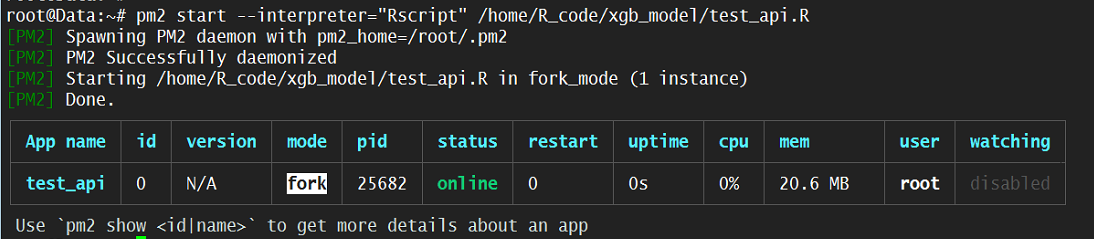
\includegraphics{pic/plumber/1.png}

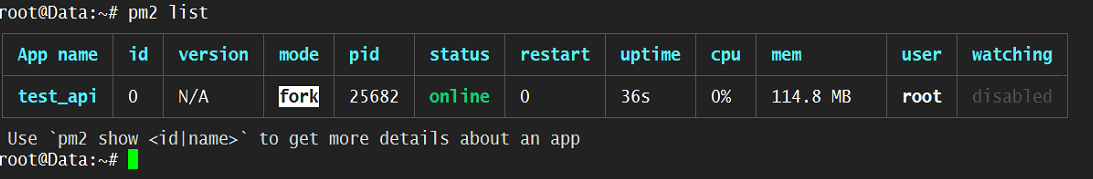
\includegraphics{pic/plumber/2.png}

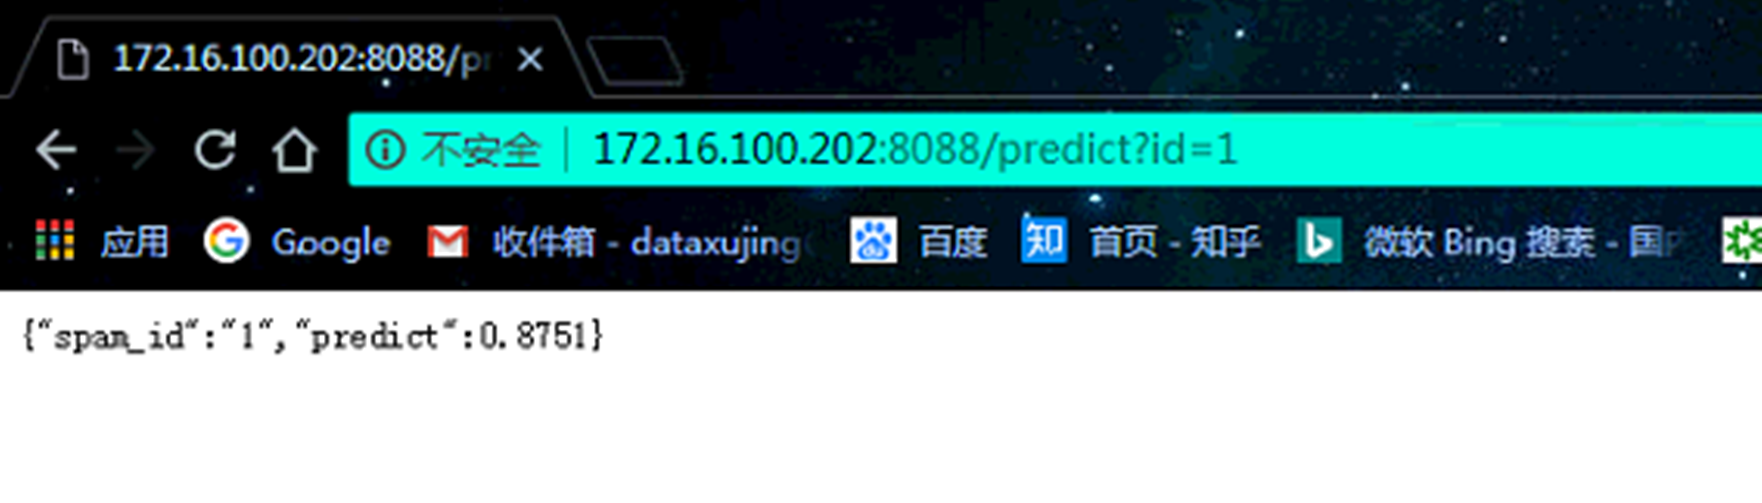
\includegraphics{pic/plumber/3.png}

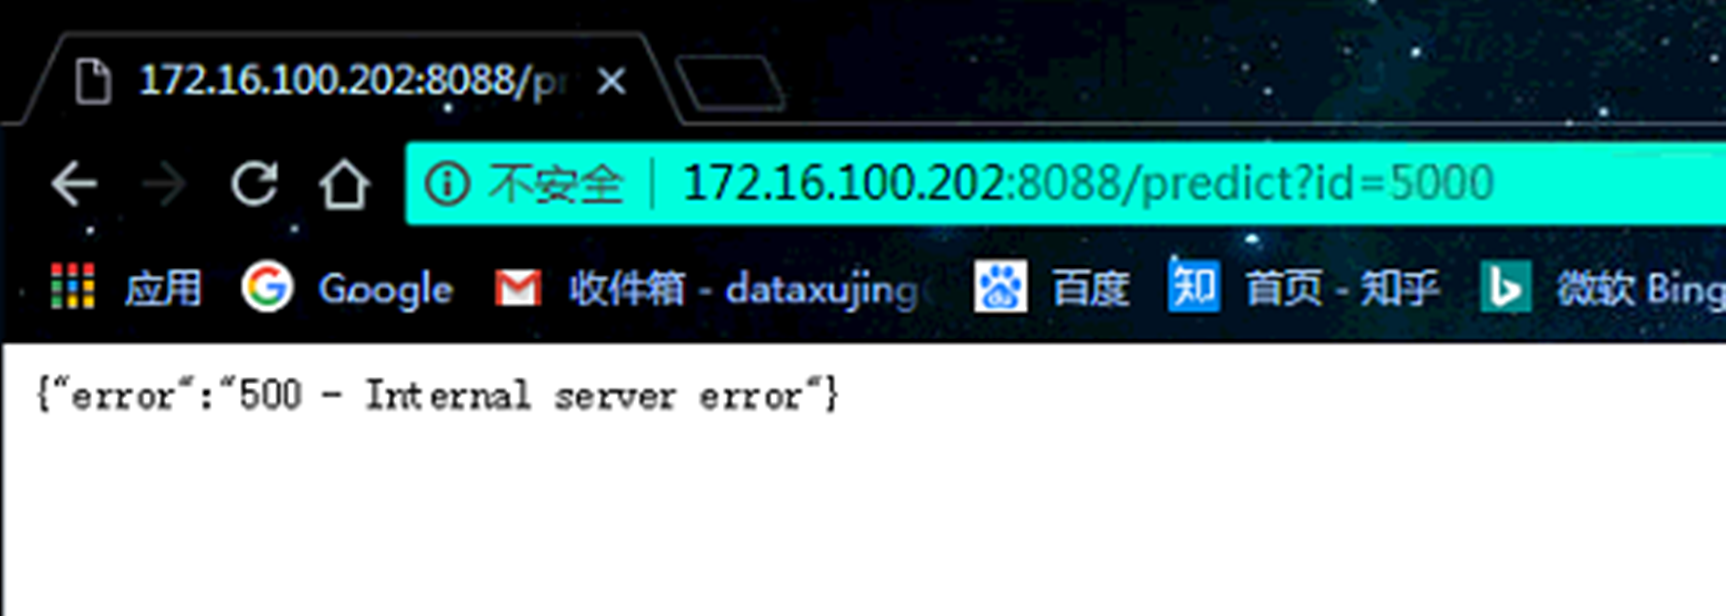
\includegraphics{pic/plumber/4.png}

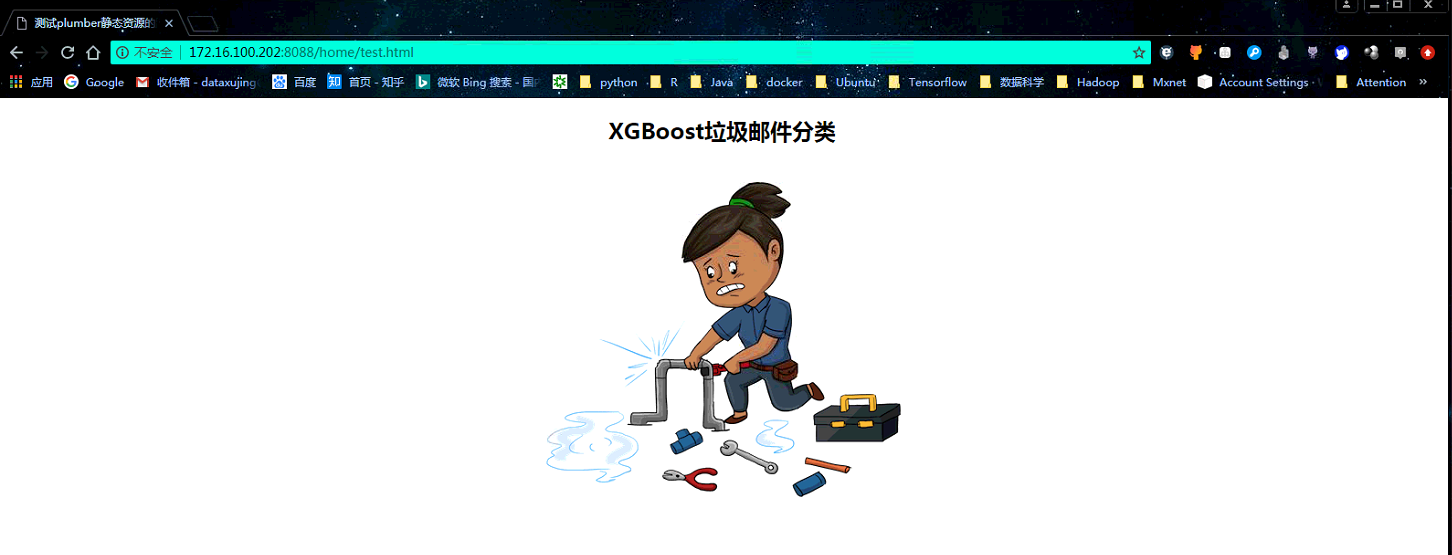
\includegraphics{pic/plumber/6.png}

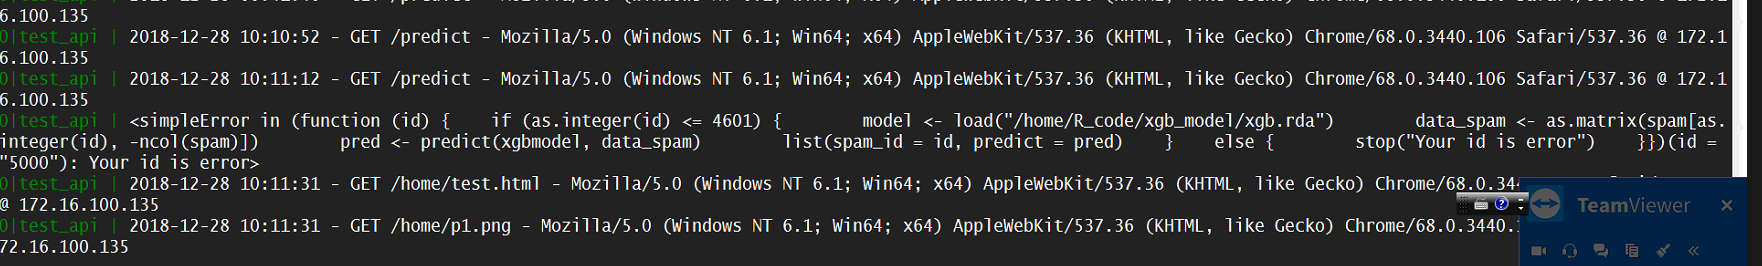
\includegraphics{pic/plumber/7.png}

\section{其他}

\subsection{环境}

当你plumb()是一个文件时,Plumber会调用source()该文件来评估你定义的任何顶级代码。

\begin{Shaded}
\begin{Highlighting}[]
\CommentTok{# Global code; gets executed at plumb() time.}
\NormalTok{counter <-}\StringTok{ }\DecValTok{0}

\CommentTok{#' @get /}
\ControlFlowTok{function}\NormalTok{()\{}
  \CommentTok{# Only gets evaluated when this endpoint is requested.}
\NormalTok{  counter <<-}\StringTok{ }\NormalTok{counter }\OperatorTok{+}\StringTok{ }\DecValTok{1}
\NormalTok{\}}
\end{Highlighting}
\end{Shaded}

counter则将创建变量,该变量将存在于为此API创建的环境中,每访问一次counter就加1,此技术允许所有端点和过滤器共享在API顶层定义的某些数据。

默认情况下,每个路由和子路由都会创建自己的环境,如果要共享环境,则在创建路由器时需要提供单个共享环境。关于环境的介绍可以参考我的R语言面向对象的编程。

\subsection{文件系统}

写入文件过程中的并发性是不可靠的,举个简单的例子,如果您已经将API水平扩展到五个R进程,那么两个转到write.csv()同时,你会看到一个进程的数据被另一个进程立即覆盖,或者
- 更糟糕的是 -
你可能最终得到一个无法读取的损坏的CSV文件。不要依赖文件系统来协调并发运行的单个R进程的共享状态。还有就是要注意,有些平台可能不具备磁盘持久化。

协调API状态时要考虑的最后一个选项是利用外部数据存储。这可以是关系数据库(如MySQL),非关系数据库(如MongoDB),也可以是Redis等事务数据存储。

任何这些选项的一个重要考虑因素是确保它们是``事务性的'',这意味着两个试图同时写入的Plumber进程不会相互覆盖。如果你对此感兴趣,可在\url{https://db.rstudio.com/}看一些的的介绍

如果在终止Plumber流程时有一个需要清理的数据库连接池。您可以使用exit钩子来定义这样的处理程序

\begin{Shaded}
\begin{Highlighting}[]
\NormalTok{pr <-}\StringTok{ }\KeywordTok{plumb}\NormalTok{(}\StringTok{"plumber.R"}\NormalTok{)}
\NormalTok{pr}\OperatorTok{$}\KeywordTok{registerHook}\NormalTok{(}\StringTok{"exit"}\NormalTok{, }\ControlFlowTok{function}\NormalTok{()\{}
  \KeywordTok{print}\NormalTok{(}\StringTok{"Bye bye!"}\NormalTok{)}
\NormalTok{\})}
\NormalTok{pr}\OperatorTok{$}\KeywordTok{run}\NormalTok{()}
\end{Highlighting}
\end{Shaded}

当您中断API时(例如,通过Escape按键或Ctrl+C),您将看到Bye
bye!打印到控制台。您甚至可以注册多个exit挂钩,它们将按照注册顺序运行。

\subsection{API的安全性}\label{api}

\subsubsection{网络和防火墙}

防火墙是一种阻止不受欢迎的网络流量的方法。大多数台式计算机和许多服务器都带有开箱即用的防火墙。这意味着如果要公开在端口8000上运行的API,则需要将防火墙配置为接受该端口上的传入连接。防火墙也可以在其他网络中介上配置,因此您可能需要配置多个防火墙以允许流量通过,以便向API客户端公开所需的端口。

\subsubsection{拒绝服务(DoS)}\label{dos}

使用拒绝服务(DoS)攻击是为了通过流量压缩服务器或服务来暂时关闭服务器或服务。DoS场景可能是由单个无知用户无意中发出可能要求服务器执行某项不可能完成任务的请求引起的,或者可能是由恶意行为者故意引入,利用大量机器重复发出昂贵的请求。服务器响应。

在设计Plumber
API时,应该采用一些做法,以便围绕API请求可能发起的工作提供安全保护。

\begin{Shaded}
\begin{Highlighting}[]
\CommentTok{#' This is an example of an UNSAFE endpoint which}
\CommentTok{#' is vulnerable to a DOS attack.}
\CommentTok{#' @get /}
\CommentTok{#' @png}
\ControlFlowTok{function}\NormalTok{(}\DataTypeTok{pts=}\DecValTok{10}\NormalTok{) \{}
  \CommentTok{# An example of an UNSAFE endpoint.}
  \KeywordTok{plot}\NormalTok{(}\DecValTok{1}\OperatorTok{:}\NormalTok{pts)}
\NormalTok{\}}
\end{Highlighting}
\end{Shaded}

\begin{Shaded}
\begin{Highlighting}[]
\CommentTok{#' This is an example of an safe endpoint which}
\CommentTok{#' checks user input to avoid a DOS attack}
\CommentTok{#' @get /}
\CommentTok{#' @png}
\ControlFlowTok{function}\NormalTok{(}\DataTypeTok{pts=}\DecValTok{10}\NormalTok{) \{}
  \ControlFlowTok{if}\NormalTok{ (pts }\OperatorTok{>}\StringTok{ }\DecValTok{1000}\NormalTok{)\{}
    \KeywordTok{stop}\NormalTok{(}\StringTok{"pts must be < 1,000"}\NormalTok{)}
\NormalTok{  \}}

  \KeywordTok{plot}\NormalTok{(}\DecValTok{1}\OperatorTok{:}\NormalTok{pts)}
\NormalTok{\}}
\end{Highlighting}
\end{Shaded}

在这里,可以看到我们只允许用户请求最多1,000个点的图表。超过该限制的任何请求将立即终止,无需进一步计算。

还有其他的,比如限制文件读取,跨站请求伪造等,可以详细参考一些前端的知识,如果你只是在企业内部内网环境中构建接口,可暂时不考虑这些内容。

\subsection{创建和控制路由器}

要以编程方式实例化新的Plumber路由器,您可以调用plumber\$new()。这将返回一个没有端点的空白Plumber路由器。您可以调用run()返回的对象来启动API,但它不知道如何响应任何请求,因此任何传入流量都会得到404响应。

\subsection{定义端点}

可以使用该handle()方法在路由器上定义端点。例如,要定义响应GET请求/和POST请求的Plumber
API /submit,您可以使用以下代码:

\begin{Shaded}
\begin{Highlighting}[]
\NormalTok{pr <-}\StringTok{ }\NormalTok{plumber}\OperatorTok{$}\KeywordTok{new}\NormalTok{()}
\NormalTok{pr}\OperatorTok{$}\KeywordTok{handle}\NormalTok{(}\StringTok{"GET"}\NormalTok{, }\StringTok{"/"}\NormalTok{, }\ControlFlowTok{function}\NormalTok{(req, res)\{}
  \CommentTok{# ...}
\NormalTok{\})}

\NormalTok{pr}\OperatorTok{$}\KeywordTok{handle}\NormalTok{(}\StringTok{"POST"}\NormalTok{, }\StringTok{"/submit"}\NormalTok{, }\ControlFlowTok{function}\NormalTok{(req, res)\{}
  \CommentTok{# ...}
\NormalTok{\})}
\end{Highlighting}
\end{Shaded}

如果使用注释来定义API,则在这些handle调用中定义的``处理程序''函数与您在plumber.R文件中定义的代码相同。

该handle()方法采用其他参数,允许您控制端点的细微差别行为,例如它可能抢占哪个过滤器或应该使用哪个序列化程序。例如,以下端点将使用Plumber的HTML序列化程序。

\begin{Shaded}
\begin{Highlighting}[]
\NormalTok{pr <-}\StringTok{ }\NormalTok{plumber}\OperatorTok{$}\KeywordTok{new}\NormalTok{()}
\NormalTok{pr}\OperatorTok{$}\KeywordTok{handle}\NormalTok{(}\StringTok{"GET"}\NormalTok{, }\StringTok{"/"}\NormalTok{, }\ControlFlowTok{function}\NormalTok{()\{}
  \StringTok{"<html><h1>Programmatic Plumber!</h1></html>"}
\NormalTok{\}, }\DataTypeTok{serializer=}\NormalTok{plumber}\OperatorTok{::}\KeywordTok{serializer_html}\NormalTok{())}
\end{Highlighting}
\end{Shaded}

\subsection{定义过滤器}

使用filter()Plumber路由器的方法定义新的过滤器:

\begin{Shaded}
\begin{Highlighting}[]
\NormalTok{pr <-}\StringTok{ }\NormalTok{plumber}\OperatorTok{$}\KeywordTok{new}\NormalTok{()}

\NormalTok{pr}\OperatorTok{$}\KeywordTok{filter}\NormalTok{(}\StringTok{"myFilter"}\NormalTok{, }\ControlFlowTok{function}\NormalTok{(req)\{}
\NormalTok{  req}\OperatorTok{$}\NormalTok{filtered <-}\StringTok{ }\OtherTok{TRUE}
  \KeywordTok{forward}\NormalTok{()}
\NormalTok{\})}

\NormalTok{pr}\OperatorTok{$}\KeywordTok{handle}\NormalTok{(}\StringTok{"GET"}\NormalTok{, }\StringTok{"/"}\NormalTok{, }\ControlFlowTok{function}\NormalTok{(req)\{}
  \KeywordTok{paste}\NormalTok{(}\StringTok{"Am I filtered?"}\NormalTok{, req}\OperatorTok{$}\NormalTok{filtered)}
\NormalTok{\})}
\end{Highlighting}
\end{Shaded}

\subsection{在路由器上注册钩子(*)}

plumber路由器支持``钩子''的概念,可以注册这些钩子以在请求的生命周期中的特定点执行某些代码。Plumber路由器目前支持四个钩子:

\begin{itemize}
\item
  preroute(data, req, res)
\item
  postroute(data, req, res, value)
\item
  preserialize(data, req, res, value)
\item
  postserialize(data, req, res, value)
\end{itemize}

在上述所有情况中,您可以访问data参数中的一次性环境,该参数作为每个请求的临时数据存储创建。钩子可以在这些钩子中存储临时数据,这些钩子可以被处理同一请求的其他钩子重用。

在Plumber路由器中定义钩子时的一个特性是能够修改返回的值。这种钩子的约定是:任何接受命名参数的函数value都应该返回新值。这可能是传入的值的未修改版本,也可能是变异值。但在任何一种情况下,如果你的钩子接受一个参数value,那么你的钩子返回的任何东西都将被用作响应的新值。

您可以使用该registerHook方法添加钩子,也可以使用registerHooks带有名称列表的方法一次添加多个钩子,其中名称是钩子的名称,值是处理程序本身。

\begin{Shaded}
\begin{Highlighting}[]

\NormalTok{pr <-}\StringTok{ }\NormalTok{plumber}\OperatorTok{$}\KeywordTok{new}\NormalTok{()}
\NormalTok{pr}\OperatorTok{$}\KeywordTok{registerHook}\NormalTok{(}\StringTok{"preroute"}\NormalTok{, }\ControlFlowTok{function}\NormalTok{(req)\{}
  \KeywordTok{cat}\NormalTok{(}\StringTok{"Routing a request for"}\NormalTok{, req}\OperatorTok{$}\NormalTok{PATH_INFO, }\StringTok{"...}\CharTok{\textbackslash{}n}\StringTok{"}\NormalTok{)}
\NormalTok{\})}
\NormalTok{pr}\OperatorTok{$}\KeywordTok{registerHooks}\NormalTok{(}\KeywordTok{list}\NormalTok{(}
  \DataTypeTok{preserialize=}\ControlFlowTok{function}\NormalTok{(req, value)\{}
    \KeywordTok{print}\NormalTok{(}\StringTok{"About to serialize this value:"}\NormalTok{)}
    \KeywordTok{print}\NormalTok{(value)}
    
    \CommentTok{# Must return the value since we took one in. Here we're not choosing}
    \CommentTok{# to mutate it, but we could.}
\NormalTok{    value}
\NormalTok{  \},}
  \DataTypeTok{postserialize=}\ControlFlowTok{function}\NormalTok{(res)\{}
    \KeywordTok{print}\NormalTok{(}\StringTok{"We serialized the value as:"}\NormalTok{)}
    \KeywordTok{print}\NormalTok{(res}\OperatorTok{$}\NormalTok{body)}
\NormalTok{  \}}
\NormalTok{))}

\NormalTok{pr}\OperatorTok{$}\KeywordTok{handle}\NormalTok{(}\StringTok{"GET"}\NormalTok{, }\StringTok{"/"}\NormalTok{, }\ControlFlowTok{function}\NormalTok{()\{ }\DecValTok{123}\NormalTok{ \})}
\end{Highlighting}
\end{Shaded}

发出GET请求/将从我们注册的三个事件中打印出各种信息。

\subsection{Mounting \& Static File
Routers(*)}\label{mounting-static-file-routers}

plumber路由器可以通过使用mount()方法通过路径划分API,这是将大型API分解为较小文件的绝佳技术。

\begin{Shaded}
\begin{Highlighting}[]
\NormalTok{root <-}\StringTok{ }\NormalTok{plumber}\OperatorTok{$}\KeywordTok{new}\NormalTok{()}

\NormalTok{users <-}\StringTok{ }\NormalTok{plumber}\OperatorTok{$}\KeywordTok{new}\NormalTok{(}\StringTok{"users.R"}\NormalTok{)}
\NormalTok{root}\OperatorTok{$}\KeywordTok{mount}\NormalTok{(}\StringTok{"/users"}\NormalTok{, users)}

\NormalTok{products <-}\StringTok{ }\NormalTok{plumber}\OperatorTok{$}\KeywordTok{new}\NormalTok{(}\StringTok{"products.R"}\NormalTok{)}
\NormalTok{root}\OperatorTok{$}\KeywordTok{mount}\NormalTok{(}\StringTok{"/products"}\NormalTok{, products)}
\end{Highlighting}
\end{Shaded}

这与用于定义提供静态文件目录的路由器的方法相同。静态文件路由器只是使用创建的Plumber路由器的一个特例PlumberStatic\$new()。例如

\begin{Shaded}
\begin{Highlighting}[]
\NormalTok{pr <-}\StringTok{ }\NormalTok{plumber}\OperatorTok{$}\KeywordTok{new}\NormalTok{()}

\NormalTok{stat <-}\StringTok{ }\NormalTok{PlumberStatic}\OperatorTok{$}\KeywordTok{new}\NormalTok{(}\StringTok{"./myfiles"}\NormalTok{)}

\NormalTok{pr}\OperatorTok{$}\KeywordTok{mount}\NormalTok{(}\StringTok{"/assets"}\NormalTok{, stat)}
\end{Highlighting}
\end{Shaded}

这将使存储在./myfiles目录中的文件和目录在API的/assets/路径下可用。

\subsection{自定义路由器}

还可以使用以下任何一种方法修改路由器的行为:

\begin{itemize}
\tightlist
\item
  setSerializer() - 设置路由器的默认序列化程序。
\item
  setErrorHandler() -
  设置在任何过滤器或端点生成错误时调用的错误处理程序。
\item
  set404Handler() -
  设置在任何过滤器,端点或子路由器无法提供传入请求时调用的处理程序。
\end{itemize}

\subsection{调试}

\subsubsection{打印调试}

大多数程序员首先通过在代码中添加print语句来进行调试,以便在某些时候检查状态。在R中,print()或者cat()可以用来打印出一些状态。例如,cat(``i
is currently:'',
i)可以在代码中插入,以帮助您确保变量i是代码中该位置的变量。

这种方法在Plumber同样可行。在交互式环境中开发Plumber
API时,此调试输出将记录到您调用run()API
的同一终端。在非交互式生产环境中,这些消息将包含在API服务器日志中以供以后检查。

\subsubsection{交互式调试}

在本地开发API时通过browser()在其中一个过滤器或端点中添加调用,然后在客户端中访问API来利用。当您想要检查多个不同的变量或与函数内部的当前状态进行交互时,这提供了一种强大的技术。

\begin{Shaded}
\begin{Highlighting}[]
\CommentTok{#' @get /}
\ControlFlowTok{function}\NormalTok{(req, res)\{}
  \KeywordTok{browser}\NormalTok{()}
  
  \KeywordTok{list}\NormalTok{(}\DataTypeTok{a=}\DecValTok{123}\NormalTok{)}
\NormalTok{\}}
\end{Highlighting}
\end{Shaded}

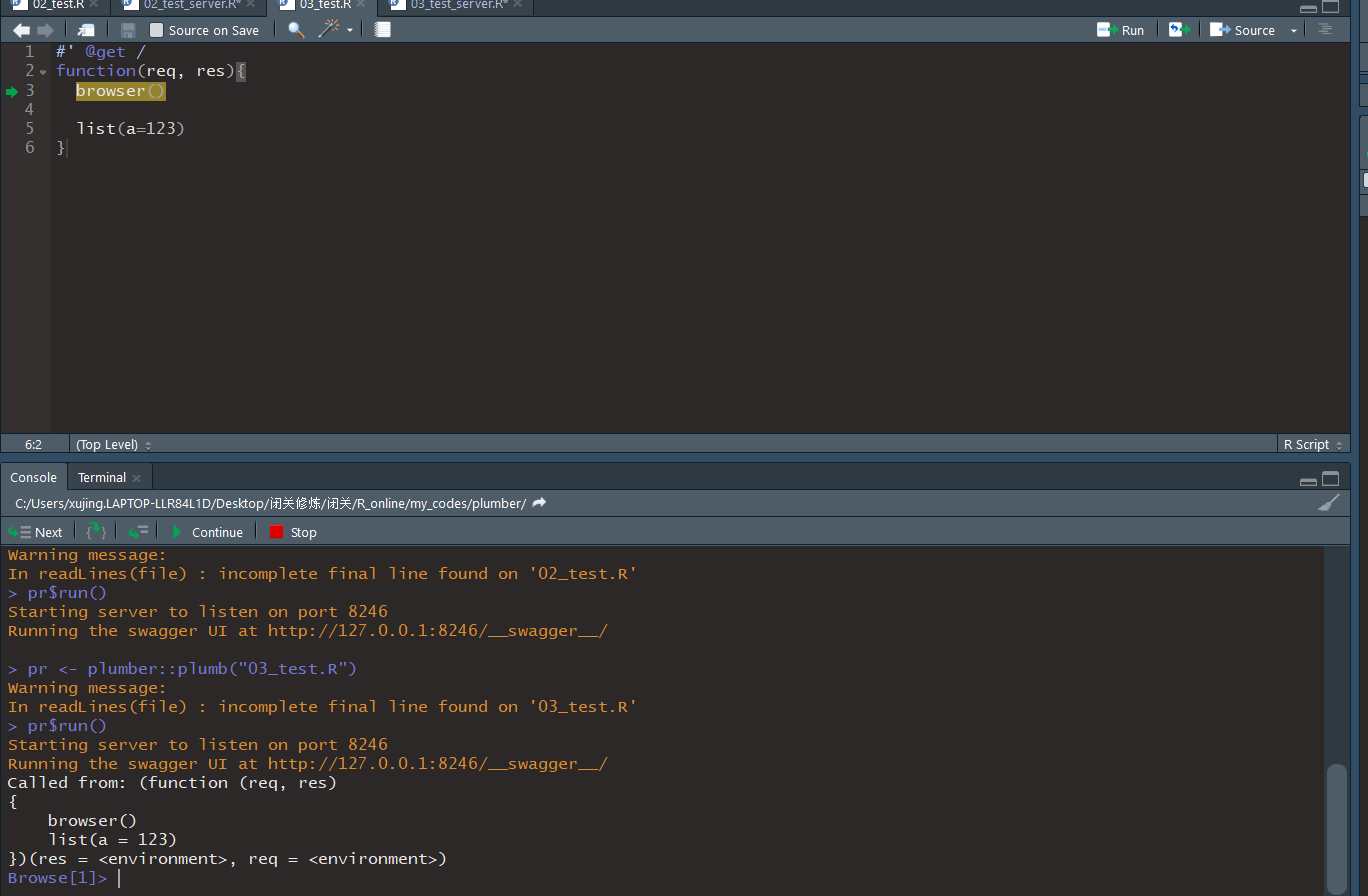
\includegraphics{pic/plumber/p6.png}

\chapter{jug}\label{jug}

\section{What is jug?}\label{what-is-jug}

jug是一个微型的轻量级的框架,基于httpuv包,为的是部署你的R代码更简单。

jug不会是一个高效的框架,它的作用是让你轻松的为你的R代码创建API,
jug的简单灵活,理论上你可以用其构建一个更一般的Web应用。

\hypertarget{install-and-hello-world}{\section{Install and Hello
World}\label{install-and-hello-world}}

要安装最新版本,请使用devtools:

\begin{Shaded}
\begin{Highlighting}[]
\NormalTok{devtools}\OperatorTok{::}\KeywordTok{install_github}\NormalTok{(}\StringTok{"Bart6114/jug"}\NormalTok{)}

\CommentTok{# jug.parallel允许jug并行处理请求}
\NormalTok{devtools }\OperatorTok{::}\StringTok{ }\NormalTok{install_github(“Bart6114}\OperatorTok{/}\NormalTok{jug.parallel”)}
\end{Highlighting}
\end{Shaded}

或者安装CRAN版本:

\begin{Shaded}
\begin{Highlighting}[]
\KeywordTok{install.packags}\NormalTok{(}\StringTok{"jug"}\NormalTok{)}
\end{Highlighting}
\end{Shaded}

加载库:

\begin{Shaded}
\begin{Highlighting}[]
\KeywordTok{library}\NormalTok{(jug)}
\KeywordTok{library}\NormalTok{(jug.parallel)}
\end{Highlighting}
\end{Shaded}

\begin{Shaded}
\begin{Highlighting}[]
\CommentTok{# Example1}
\KeywordTok{jug}\NormalTok{()}
\end{Highlighting}
\end{Shaded}

\begin{Shaded}
\begin{Highlighting}[]
\CommentTok{# Example2}
\KeywordTok{library}\NormalTok{(jug)}

\KeywordTok{jug}\NormalTok{() }\OperatorTok
\StringTok{  }\KeywordTok{get}\NormalTok{(}\StringTok{"/"}\NormalTok{, }\ControlFlowTok{function}\NormalTok{(req, res, err)\{}
    \StringTok{"Hello World!"}
\NormalTok{  \}) }\OperatorTok
\StringTok{  }\KeywordTok{simple_error_handler_json}\NormalTok{() }\OperatorTok
\StringTok{  }\KeywordTok{serve_it}\NormalTok{()}
\end{Highlighting}
\end{Shaded}

\begin{Shaded}
\begin{Highlighting}[]
\CommentTok{# Example3}
\KeywordTok{library}\NormalTok{(jug)}

\KeywordTok{jug}\NormalTok{() }\OperatorTok
\StringTok{  }\KeywordTok{get}\NormalTok{(}\StringTok{"/"}\NormalTok{, }\ControlFlowTok{function}\NormalTok{(req, res, err)\{}
    \StringTok{"Hello World!"}
\NormalTok{  \}) }\OperatorTok
\StringTok{  }\KeywordTok{simple_error_handler_json}\NormalTok{() }\OperatorTok
\StringTok{  }\KeywordTok{serve_it_parallel}\NormalTok{(}\DataTypeTok{processes=}\DecValTok{8}\NormalTok{)}
\end{Highlighting}
\end{Shaded}

\begin{Shaded}
\begin{Highlighting}[]
\KeywordTok{kill_servers}\NormalTok{()}
\end{Highlighting}
\end{Shaded}

jug与magrittr(\%\textgreater{}\%)的管道功能密切配合。

\section{Middleware(中间件)}\label{middleware}

在中间件方面,jug有遵循中间件的规范Express。在jug中,中间件是一个可以访问\texttt{request(req)},\texttt{response(res)}和\texttt{error(err)}对象的函数。

可以定义多个中间件。中间件的添加顺序很重要。请求将从添加的第一个中间件(更具体地说是在其中指定的函数
-
请参见下一段)开始。它将继续通过添加的中间件传递,直到中间件不返回NULL。

\subsection{方法不敏感的中间件}

该\texttt{use}函数是一个方法不敏感的中间件说明符。虽然它对方法不敏感,但它可以绑定到特定路径。如果path参数(接受带grepl设置的正则表达式字符串perl=TRUE)如果设置为NULL,它也会变得路径不敏感,并将处理每个请求。

路径不敏感的栗子:

\begin{Shaded}
\begin{Highlighting}[]
\KeywordTok{jug}\NormalTok{() }\OperatorTok
\StringTok{  }\KeywordTok{use}\NormalTok{(}\DataTypeTok{path =} \OtherTok{NULL}\NormalTok{, }\ControlFlowTok{function}\NormalTok{(req, res, err)\{}
    \StringTok{"test 1,2,3!"}
\NormalTok{    \}) }\OperatorTok
\StringTok{  }\KeywordTok{serve_it}\NormalTok{()}
  
\end{Highlighting}
\end{Shaded}

\begin{Shaded}
\begin{Highlighting}[]
\OperatorTok{$}\StringTok{ }\NormalTok{curl }\FloatTok{127.0}\NormalTok{.}\FloatTok{0.1}\OperatorTok{:}\DecValTok{8080}\OperatorTok{/}\NormalTok{xyz}
\NormalTok{test }\DecValTok{1}\NormalTok{,}\DecValTok{2}\NormalTok{,}\DecValTok{3}\OperatorTok{!}
\end{Highlighting}
\end{Shaded}

同样的栗子,但是路径敏感:

\begin{Shaded}
\begin{Highlighting}[]
\KeywordTok{jug}\NormalTok{() }\OperatorTok
\StringTok{  }\KeywordTok{use}\NormalTok{(}\DataTypeTok{path =} \StringTok{"/"}\NormalTok{, }\ControlFlowTok{function}\NormalTok{(req, res, err)\{}
    \StringTok{"test 1,2,3!"}
\NormalTok{    \}) }\OperatorTok
\StringTok{  }\KeywordTok{serve_it}\NormalTok{()}
\end{Highlighting}
\end{Shaded}

\begin{Shaded}
\begin{Highlighting}[]
\OperatorTok{$}\StringTok{ }\NormalTok{curl }\FloatTok{127.0}\NormalTok{.}\FloatTok{0.1}\OperatorTok{:}\DecValTok{8080}\OperatorTok{/}\NormalTok{xyz}
\NormalTok{curl}\OperatorTok{:}\StringTok{ }\NormalTok{(}\DecValTok{52}\NormalTok{) Empty reply from server}

\OperatorTok{$}\StringTok{ }\NormalTok{curl }\FloatTok{127.0}\NormalTok{.}\FloatTok{0.1}\OperatorTok{:}\DecValTok{8080}
\NormalTok{test }\DecValTok{1}\NormalTok{,}\DecValTok{2}\NormalTok{,}\DecValTok{3}\OperatorTok{!}
\end{Highlighting}
\end{Shaded}

请注意,在上面的示例中,缺少错误/缺少路由处理(服务器可能崩溃/不响应),稍后将详细介绍.

\subsection{方法敏感的中间件}

与请求方法不敏感的中间件相同的样式,有可用的请求方法敏感中间件。更具体地讲,您可以使用\texttt{get},\texttt{post},\texttt{put}和\texttt{delete}功能。

此类中间件使用path参数绑定到路径。如果path设置为NULL,它将绑定到路径的每个请求,对应相应的请求方法。

\begin{Shaded}
\begin{Highlighting}[]
\KeywordTok{jug}\NormalTok{() }\OperatorTok
\StringTok{  }\KeywordTok{get}\NormalTok{(}\DataTypeTok{path =} \StringTok{"/"}\NormalTok{, }\ControlFlowTok{function}\NormalTok{(req, res, err)\{}
    \StringTok{"get test 1,2,3!"}
\NormalTok{    \}) }\OperatorTok
\StringTok{  }\KeywordTok{serve_it}\NormalTok{()}
\end{Highlighting}
\end{Shaded}

\begin{Shaded}
\begin{Highlighting}[]
\OperatorTok{$}\StringTok{ }\NormalTok{curl }\FloatTok{127.0}\NormalTok{.}\FloatTok{0.1}\OperatorTok{:}\DecValTok{8080}
\NormalTok{get test }\DecValTok{1}\NormalTok{,}\DecValTok{2}\NormalTok{,}\DecValTok{3}\OperatorTok{!}
\end{Highlighting}
\end{Shaded}

中间件意味着被链接,因此要将不同的功能绑定到不同的路径:

\begin{Shaded}
\begin{Highlighting}[]
\KeywordTok{jug}\NormalTok{() }\OperatorTok
\StringTok{  }\KeywordTok{get}\NormalTok{(}\DataTypeTok{path =} \StringTok{"/"}\NormalTok{, }\ControlFlowTok{function}\NormalTok{(req, res, err)\{}
    \StringTok{"get test 1,2,3 on path /"}
\NormalTok{    \}) }\OperatorTok
\StringTok{  }\KeywordTok{get}\NormalTok{(}\DataTypeTok{path =} \StringTok{"/my_path"}\NormalTok{, }\ControlFlowTok{function}\NormalTok{(req, res, err)\{}
    \StringTok{"get test 1,2,3 on path /my_path"}
\NormalTok{    \}) }\OperatorTok
\StringTok{  }\KeywordTok{serve_it}\NormalTok{()}
\end{Highlighting}
\end{Shaded}

\begin{Shaded}
\begin{Highlighting}[]
\OperatorTok{$}\StringTok{ }\NormalTok{curl }\FloatTok{127.0}\NormalTok{.}\FloatTok{0.1}\OperatorTok{:}\DecValTok{8080}
\NormalTok{get test }\DecValTok{1}\NormalTok{,}\DecValTok{2}\NormalTok{,}\DecValTok{3}\NormalTok{ on path }\OperatorTok{/}

\ErrorTok{$}\StringTok{ }\NormalTok{curl }\FloatTok{127.0}\NormalTok{.}\FloatTok{0.1}\OperatorTok{:}\DecValTok{8080}\OperatorTok{/}\NormalTok{my_path}
\NormalTok{get test }\DecValTok{1}\NormalTok{,}\DecValTok{2}\NormalTok{,}\DecValTok{3}\NormalTok{ on path }\OperatorTok{/}\NormalTok{my_path}
\end{Highlighting}
\end{Shaded}

\subsection{Websocket协议}\label{websocket}

默认情况下,所有中间件便利功能都绑定到http协议。但是,您可以使用websocket中间件功能通过websocket访问jug服务器ws。下面是回传传入消息的示例。

\begin{Shaded}
\begin{Highlighting}[]
\KeywordTok{jug}\NormalTok{() }\OperatorTok
\StringTok{   }\KeywordTok{ws}\NormalTok{(}\StringTok{"/echo_message"}\NormalTok{, }\ControlFlowTok{function}\NormalTok{(binary, message, res, err)\{}
\NormalTok{    message}
\NormalTok{  \}) }\OperatorTok
\StringTok{  }\KeywordTok{serve_it}\NormalTok{()}
\end{Highlighting}
\end{Shaded}

打开连接并向ws://127.0.0.1:8080/echo\_message其发送例如消息test将返回该值test。

请注意,websocket支持在此阶段是实验性的,尽量不使用jug操作websocket

\subsection{include定义其他位置的中间件}\label{include}

为了使代码更加模块化,您可以将其他定义的中间件链包含到您的jug实例中。为此,您可以使用\texttt{collector()}和\texttt{include()}功能的组合。

下面是一个collector本地定义(在相同的R脚本中)和include栗子:

\begin{Shaded}
\begin{Highlighting}[]
\NormalTok{ collected_mw<-}
\StringTok{    }\KeywordTok{collector}\NormalTok{() }\OperatorTok
\StringTok{    }\KeywordTok{get}\NormalTok{(}\StringTok{"/"}\NormalTok{, }\ControlFlowTok{function}\NormalTok{(req,res,err)\{}
      \KeywordTok{return}\NormalTok{(}\StringTok{"test"}\NormalTok{)}
\NormalTok{    \})}

\NormalTok{  res<-}\KeywordTok{jug}\NormalTok{() }\OperatorTok
\StringTok{    }\KeywordTok{include}\NormalTok{(collected_mw) }\OperatorTok
\StringTok{    }\KeywordTok{serve_it}\NormalTok{()}
\end{Highlighting}
\end{Shaded}

然而,也有可能include一个collector是在另一个.R文件中定义。

让我们说下面是文件my\_middlewares.R:

\begin{Shaded}
\begin{Highlighting}[]
\KeywordTok{library}\NormalTok{(jug)}

\NormalTok{collected_mw<-}
\StringTok{  }\KeywordTok{collector}\NormalTok{() }\OperatorTok
\StringTok{  }\KeywordTok{get}\NormalTok{(}\StringTok{"/"}\NormalTok{, }\ControlFlowTok{function}\NormalTok{(req,res,err)\{}
    \KeywordTok{return}\NormalTok{(}\StringTok{"test2"}\NormalTok{)}
\NormalTok{  \})}
\end{Highlighting}
\end{Shaded}

我们可以include如下:

\begin{Shaded}
\begin{Highlighting}[]
\NormalTok{res<-}\KeywordTok{jug}\NormalTok{() }\OperatorTok
\StringTok{  }\KeywordTok{include}\NormalTok{(collected_mw, }\StringTok{"my_middlewares.R"}\NormalTok{) }\OperatorTok
\StringTok{  }\KeywordTok{serve_it}\NormalTok{()}
\end{Highlighting}
\end{Shaded}

\section{预定义的中间件}

\subsection{错误处理}\label{-1}

一个简单的错误处理中间件(simple\_error\_handler/
simple\_error\_handler\_json),它捕获未绑定的路径和func评估错误。如果您没有实现自定义错误处理程序,我建议您将其中任何一个添加到您的jug实例中。simple\_error\_handler返回一个HTML错误页面而simple\_error\_handler\_json返回一个JSON消息。

\begin{Shaded}
\begin{Highlighting}[]
\KeywordTok{jug}\NormalTok{() }\OperatorTok
\StringTok{  }\KeywordTok{simple_error_handler}\NormalTok{() }\OperatorTok
\StringTok{  }\KeywordTok{serve_it}\NormalTok{()}
\end{Highlighting}
\end{Shaded}

\begin{Shaded}
\begin{Highlighting}[]
\OperatorTok{$}\StringTok{ }\NormalTok{curl }\FloatTok{127.0}\NormalTok{.}\FloatTok{0.1}\OperatorTok{:}\DecValTok{8080}
\OperatorTok{<!}\NormalTok{DOCTYPE html}\OperatorTok{>}
\ErrorTok{<}\NormalTok{html lang=}\StringTok{"en"}\OperatorTok{>}
\StringTok{  }\ErrorTok{<}\NormalTok{head}\OperatorTok{>}
\StringTok{    }\ErrorTok{<}\NormalTok{meta charset=}\StringTok{"utf-8"}\OperatorTok{>}
\StringTok{    }\ErrorTok{<}\NormalTok{title}\OperatorTok{>}\NormalTok{Not found}\OperatorTok{<}\ErrorTok{/}\NormalTok{title}\OperatorTok{>}
\StringTok{  }\ErrorTok{</}\NormalTok{head}\OperatorTok{>}
\StringTok{  }\ErrorTok{<}\NormalTok{body}\OperatorTok{>}
\StringTok{    }\ErrorTok{<}\NormalTok{p}\OperatorTok{>}\NormalTok{No handler bound to path}\OperatorTok{<}\ErrorTok{/}\NormalTok{p}\OperatorTok{>}
\StringTok{  }\ErrorTok{</}\NormalTok{body}\OperatorTok{>}
\ErrorTok{</}\NormalTok{html}\OperatorTok{>}
\end{Highlighting}
\end{Shaded}

如果要实现自己的自定义错误处理,只需查看这些简单错误处理中间件的代码即可。

请注意,通常您希望在指定所有其他中间件后将错误处理程序中间件附加到jug实例。

\subsection{轻松使用自己的函数}

创建jug的主要原因是可以轻松访问您自己的自定义R函数。功能decorate专门为此目的而构建。如果decorate您自己的函数,它会将请求的查询字符串中传递的所有参数转换为函数的参数。它还将所有头文件作为参数传递给函数。如果您的函数不接受\texttt{...}参数,则会删除函数未明确请求的所有查询/标头参数。如果您的功能请求req,res或err参数(或\ldots{})相应的对象将被传递。

\begin{Shaded}
\begin{Highlighting}[]
\NormalTok{say_hello<-}\ControlFlowTok{function}\NormalTok{(name)\{}\KeywordTok{paste}\NormalTok{(}\StringTok{"hello"}\NormalTok{,name,}\StringTok{"!"}\NormalTok{)\}}

\KeywordTok{jug}\NormalTok{() }\OperatorTok
\StringTok{  }\KeywordTok{get}\NormalTok{(}\StringTok{"/"}\NormalTok{, }\KeywordTok{decorate}\NormalTok{(say_hello)) }\OperatorTok
\StringTok{  }\KeywordTok{serve_it}\NormalTok{()}
\end{Highlighting}
\end{Shaded}

如果在上面,您通过name查询字符串或GET请求中的标头传递参数,它将返回如下例所示。

\begin{Shaded}
\begin{Highlighting}[]
\OperatorTok{$}\StringTok{ }\NormalTok{curl }\FloatTok{127.0}\NormalTok{.}\FloatTok{0.1}\OperatorTok{:}\DecValTok{8080}\OperatorTok{/}\NormalTok{?name=Bart}
\NormalTok{hello Bart }\OperatorTok{!}
\end{Highlighting}
\end{Shaded}

\subsection{静态文件服务器}

serve\_static\_file中间件可以提供静态文件。

\begin{Shaded}
\begin{Highlighting}[]
\KeywordTok{jug}\NormalTok{() }\OperatorTok
\StringTok{  }\KeywordTok{serve_static_files}\NormalTok{() }\OperatorTok
\StringTok{  }\KeywordTok{serve_it}\NormalTok{()}
\end{Highlighting}
\end{Shaded}

默认根目录是返回的目录,\texttt{setwd()}可以通过向中间件提供root\_path参数来指定serve\_static\_files.

除了开发之外,我不建议使用jug来提供静态文件。

\subsection{CORS功能(*)}\label{cors}

\href{https://developer.mozilla.org/en-US/docs/Web/HTTP/CORS}{CORS功能}(跨源资源共享)由cors()中间件功能引入。

请考虑以下示例。

\begin{Shaded}
\begin{Highlighting}[]
\KeywordTok{jug}\NormalTok{() }\OperatorTok
\StringTok{  }\KeywordTok{cors}\NormalTok{() }\OperatorTok
\StringTok{  }\KeywordTok{get}\NormalTok{(}\StringTok{"/"}\NormalTok{, }\ControlFlowTok{function}\NormalTok{(req, res, err)\{}
    \StringTok{"Hello World!"}
\NormalTok{  \}) }\OperatorTok
\StringTok{  }\KeywordTok{serve_it}\NormalTok{()}
\end{Highlighting}
\end{Shaded}

\begin{Shaded}
\begin{Highlighting}[]
\OperatorTok{$}\StringTok{ }\NormalTok{curl }\OperatorTok{-}\NormalTok{v }\FloatTok{127.0}\NormalTok{.}\FloatTok{0.1}\OperatorTok{:}\DecValTok{8080}\OperatorTok{/}
\ErrorTok{*}\StringTok{   }\NormalTok{Trying }\FloatTok{127.0}\NormalTok{.}\FloatTok{0.1}\NormalTok{...}
\OperatorTok{*}\StringTok{ }\NormalTok{Connected to }\FloatTok{127.0}\NormalTok{.}\FloatTok{0.1}\NormalTok{ (}\FloatTok{127.0}\NormalTok{.}\FloatTok{0.1}\NormalTok{) port }\DecValTok{8080}\NormalTok{ (}\CommentTok{#0)}
\OperatorTok{>}\StringTok{ }\NormalTok{GET }\OperatorTok{/}\StringTok{ }\NormalTok{HTTP}\OperatorTok{/}\FloatTok{1.1}
\OperatorTok{>}\StringTok{ }\NormalTok{Host}\OperatorTok{:}\StringTok{ }\FloatTok{127.0}\NormalTok{.}\FloatTok{0.1}\OperatorTok{:}\DecValTok{8080}
\OperatorTok{>}\StringTok{ }\NormalTok{User}\OperatorTok{-}\NormalTok{Agent}\OperatorTok{:}\StringTok{ }\NormalTok{curl}\OperatorTok{/}\FloatTok{7.43}\NormalTok{.}\DecValTok{0}
\OperatorTok{>}\StringTok{ }\NormalTok{Accept}\OperatorTok{:}\StringTok{ }\ErrorTok{*/*}
\ErrorTok{>}\StringTok{ }
\ErrorTok{<}\StringTok{ }\NormalTok{HTTP}\OperatorTok{/}\FloatTok{1.1} \DecValTok{200}\NormalTok{ OK}
\OperatorTok{<}\StringTok{ }\NormalTok{Content}\OperatorTok{-}\NormalTok{Type}\OperatorTok{:}\StringTok{ }\NormalTok{text}\OperatorTok{/}\NormalTok{html}
\OperatorTok{<}\StringTok{ }\NormalTok{Access}\OperatorTok{-}\NormalTok{Control}\OperatorTok{-}\NormalTok{Allow}\OperatorTok{-}\NormalTok{Origin}\OperatorTok{:}\StringTok{ }\ErrorTok{*}
\ErrorTok{<}\StringTok{ }\NormalTok{Access}\OperatorTok{-}\NormalTok{Control}\OperatorTok{-}\NormalTok{Allow}\OperatorTok{-}\NormalTok{Methods}\OperatorTok{:}\StringTok{ }\NormalTok{POST,GET,PUT,OPTIONS,DELETE,PATCH}
\OperatorTok{<}\StringTok{ }\NormalTok{Content}\OperatorTok{-}\NormalTok{Length}\OperatorTok{:}\StringTok{ }\DecValTok{12}
\OperatorTok{<}\StringTok{ }
\ErrorTok{*}\StringTok{ }\NormalTok{Connection }\CommentTok{#0 to host 127.0.0.1 left intact}
\end{Highlighting}
\end{Shaded}

如您所见,这会添加一些默认的CORS标头。查看?cors配置选项,请注意您还可以通过指定path参数将CORS标头添加到特定路径。

\subsection{认证}

目前,只有通过中间件功能内置支持基本身份验证\url{https://www.httpwatch.com/httpgallery/authentication/}
auth\_basic,间件将检查有效用户名/密码组合的请求。如果传递了无效组合,它将返回401状态,WWW-Authenticate标题和文本正文,指出存在身份验证错误。

首先,您需要定义一个接受username和password参数的函数。TRUE如果组合有效且FALSE组合无效,则应返回功能。一个虚拟的例子如下所示。注意,此功能还可以检查例如数据库以验证组合。

\begin{Shaded}
\begin{Highlighting}[]
\CommentTok{# dummy account checker}
\NormalTok{account_checker <-}\StringTok{ }\ControlFlowTok{function}\NormalTok{(username, password)\{}
  \CommentTok{# do something to verify the username and password and return TRUE if combination OK}
  \KeywordTok{all}\NormalTok{(username }\OperatorTok{==}\StringTok{ "test_user"}\NormalTok{, }
\NormalTok{      password }\OperatorTok{==}\StringTok{ "test_password"}\NormalTok{)}
\NormalTok{\}}
\end{Highlighting}
\end{Shaded}

接下来,您需要auth\_basic在中间件链中实例化中间件。该auth\_basic函数接受用户名/密码验证功能作为第一个参数。下面给出两个例子。第一个显示如何对特定路径(/test)进行身份验证。

\begin{Shaded}
\begin{Highlighting}[]
\KeywordTok{jug}\NormalTok{() }\OperatorTok
\StringTok{  }\KeywordTok{get}\NormalTok{(}\StringTok{"/"}\NormalTok{, }\ControlFlowTok{function}\NormalTok{(req, res, err)\{}
    \StringTok{"/ req"}
\NormalTok{  \}) }\OperatorTok
\StringTok{  }\KeywordTok{get}\NormalTok{(}\StringTok{"/test"}\NormalTok{, }\KeywordTok{auth_basic}\NormalTok{(account_checker), }\ControlFlowTok{function}\NormalTok{(req, res, err)\{}
    \StringTok{"/test req"}
\NormalTok{  \}) }\OperatorTok
\StringTok{  }\KeywordTok{serve_it}\NormalTok{()}
\end{Highlighting}
\end{Shaded}

下面的第二个示例显示了如何为jug实例中的所有路径激活基本身份验证。

\begin{Shaded}
\begin{Highlighting}[]
\KeywordTok{jug}\NormalTok{() }\OperatorTok
\StringTok{  }\KeywordTok{use}\NormalTok{(}\OtherTok{NULL}\NormalTok{, }\KeywordTok{auth_basic}\NormalTok{(account_checker)) }\OperatorTok
\StringTok{  }\KeywordTok{get}\NormalTok{(}\StringTok{"/"}\NormalTok{, }\ControlFlowTok{function}\NormalTok{(req, res, err)\{}
    \StringTok{"/ req"}
\NormalTok{  \}) }\OperatorTok
\StringTok{  }\KeywordTok{serve_it}\NormalTok{()}
\end{Highlighting}
\end{Shaded}

\section{事件监听}

从版本0.1.7.902开始,事件监听的概念已经可用。由于中间件不足以实现强大的Logger,因此引入了事件和事件监听的概念。目前,侦听器可以绑定到事件,下面给出一个示例:

\begin{Shaded}
\begin{Highlighting}[]
\KeywordTok{jug}\NormalTok{() }\OperatorTok
\StringTok{  }\KeywordTok{get}\NormalTok{(}\StringTok{"/"}\NormalTok{, }\ControlFlowTok{function}\NormalTok{(req,res,err)\{}\StringTok{"foo"}\NormalTok{\}) }\OperatorTok
\StringTok{  }\KeywordTok{on}\NormalTok{(}\StringTok{"finish"}\NormalTok{, }\ControlFlowTok{function}\NormalTok{(req, res, err)\{}
    \KeywordTok{print}\NormalTok{(}\StringTok{"the finish event was received; request processing finished!"}\NormalTok{)\}}
\NormalTok{    ) }\OperatorTok
\StringTok{  }\KeywordTok{serve_it}\NormalTok{()}
\end{Highlighting}
\end{Shaded}

目前有三项活动:

\begin{itemize}
\tightlist
\item
  start:一旦收到新请求,就会触发此事件
\item
  finish:一旦请求完全处理,就会触发此事件
\item
  error:一旦在中间件内引发错误,就会触发此事件
\end{itemize}

start和finish事件将传递的当前状态req,res以及err对象。error事件将传递第四个参数,即错误消息的字符表示。

\section{预定义的事件侦听器}

\subsection{Logger}\label{logger}

\texttt{futile.logger}

\begin{Shaded}
\begin{Highlighting}[]
\KeywordTok{jug}\NormalTok{() }\OperatorTok
\StringTok{  }\KeywordTok{get}\NormalTok{(}\StringTok{"/"}\NormalTok{, }\ControlFlowTok{function}\NormalTok{(req,res,err)\{}\StringTok{"foo"}\NormalTok{\}) }\OperatorTok
\StringTok{  }\KeywordTok{get}\NormalTok{(}\StringTok{"/err"}\NormalTok{, }\ControlFlowTok{function}\NormalTok{(req,res,err)\{}\KeywordTok{stop}\NormalTok{(}\StringTok{"bar"}\NormalTok{)\}) }\OperatorTok
\StringTok{  }\KeywordTok{logger}\NormalTok{(}\DataTypeTok{threshold =}\NormalTok{ futile.logger}\OperatorTok{::}\NormalTok{DEBUG, }\DataTypeTok{log_file=}\StringTok{'logfile.log'}\NormalTok{, }\DataTypeTok{console=}\OtherTok{TRUE}\NormalTok{) }\OperatorTok
\StringTok{  }\KeywordTok{simple_error_handler_json}\NormalTok{() }\OperatorTok
\StringTok{  }\KeywordTok{serve_it}\NormalTok{()}
\end{Highlighting}
\end{Shaded}

在上面的示例中,Logger阈值设置futile.logger::DEBUG为我们将在执行期间接收详细信息,在这个例子中,Logger将写入logfile.log
和将输出到控制台.有关Logger阈值的更多信息,请查看该futile.logger包的文档。

\section{请求,响应和错误对象}

\subsection{Request(req)对象}\label{requestreq}

该req对象包含请求规范。它有不同的属性:

\begin{itemize}
\tightlist
\item
  \texttt{req\$params}
  由查询字符串,JSON正文,URL参数或多部分表单传递的参数的命名列表
\item
  \texttt{req\$path} 请求路径
\item
  \texttt{req\$method} 请求方法
\item
  \texttt{req\$raw} 传递的原始请求对象 httpuv
\item
  \texttt{req\$body} 完整的请求正文作为字符串
\item
  \texttt{req\$protocol}无论是http或websocket
\item
  \texttt{req\$headers}
  请求中的标头的命名列表(作为小写并从HTTP\_底层httpuv框架提供的前缀中剥离)
\end{itemize}

它附带以下功能:

\begin{itemize}
\tightlist
\item
  \texttt{req\$get\_header(key)}返回与请求中指定键关联的值(无需担心HTTP\_前缀)
\item
  \texttt{req\$set\_header(key,\ value)}
  允许在处理请求时设置/更改标头(对于将数据传递到下一个中间件可能很有用)
\item
  \texttt{req\$attach(key,\ value)} 将变量附加到 \texttt{req\$params}
\end{itemize}

\subsection{Response(res)对象}\label{responseres}

该res对象包含响应规范。它有不同的属性:

\begin{itemize}
\tightlist
\item
  \texttt{res\$headers} 一个命名的标题列表
\item
  \texttt{res\$status} 响应的状态(默认为200)
\item
  \texttt{res\$body}响应的主体(自动设置为不NULL返回的中间件的内容或通过诸如此类的方法\texttt{res\$json()})
\end{itemize}

它还有一组功能:

\begin{itemize}
\tightlist
\item
  \texttt{res\$set\_header(key,\ value)} 设置自定义标头
\item
  \texttt{res\$content\_type(type}) 设置自己的内容类型(MIME)
\item
  \texttt{res\$set\_status(status)} 设置响应的状态
\item
  \texttt{res\$text(body)} 明确地设定反应的主体
\item
  \texttt{res\$json(obj,\ auto\_unbox=TRUE)}
  将对象转换为JSON,将其设置为正文并设置正确的内容类型
\item
  \texttt{res\$plot(plot\_obj,\ base64=TRUE)}
  方便函数将绘图对象作为响应体返回,返回的绘图可以是图像的base64表示(默认)或实际的二进制数据
\end{itemize}

\subsection{Error(err)对象}\label{errorerr}

该err对象包含可通过的错误列表\texttt{err\$errrors}。您可以通过调用将错误添加到此列表中\texttt{err\$set(error)}。错误将转换为字符。有关更多详细信息,请参阅``错误处理''。

\section{URL调度}\label{url}

在路径参数get,post,\ldots{}功能被处理为正则表达式模式。

如果路径定义中有命名的捕获组,则它们将附加到该\texttt{req\$params}对象。例如,模式\texttt{/test/(?\textless{}id\textgreater{}.*)/(?\textless{}id2\textgreater{}.*)}将导致变量id和id2(及其各自的值)绑定到req\$params对象。

如果路径模式未以字符串\^{}正则表达式标记的开头启动或以字符串标记的结尾结束\texttt{\$},则将分别在路径模式规范的开头和结尾处明确地插入这些模式。例如,路径模式/将转换为\texttt{\^{}/\$}

\section{启动jug实例}\label{jug}

只需serve\_it()在管道链的末端调用(参见\protect\hyperlink{install-and-hello-world}{Install
and Hello World !}示例)

\section{线性回归模型的API举栗}\label{api}

训练mtcars数据集上的线性回归模型,并假设我们的目标是mpg根据输入gear和预测每加仑英里或变量hp。

\begin{Shaded}
\begin{Highlighting}[]
\KeywordTok{head}\NormalTok{(mtcars)}
\end{Highlighting}
\end{Shaded}

\begin{verbatim}
##                    mpg cyl disp  hp drat    wt  qsec vs am gear carb
## Mazda RX4         21.0   6  160 110 3.90 2.620 16.46  0  1    4    4
## Mazda RX4 Wag     21.0   6  160 110 3.90 2.875 17.02  0  1    4    4
## Datsun 710        22.8   4  108  93 3.85 2.320 18.61  1  1    4    1
## Hornet 4 Drive    21.4   6  258 110 3.08 3.215 19.44  1  0    3    1
## Hornet Sportabout 18.7   8  360 175 3.15 3.440 17.02  0  0    3    2
## Valiant           18.1   6  225 105 2.76 3.460 20.22  1  0    3    1
\end{verbatim}

\begin{Shaded}
\begin{Highlighting}[]
\NormalTok{mpg_model <-}\StringTok{ }\KeywordTok{lm}\NormalTok{(mpg}\OperatorTok{~}\NormalTok{gear}\OperatorTok{+}\NormalTok{hp, }\DataTypeTok{data=}\NormalTok{mtcars)}

\KeywordTok{summary}\NormalTok{(mpg_model)}
\end{Highlighting}
\end{Shaded}

\begin{verbatim}
## 
## Call:
## lm(formula = mpg ~ gear + hp, data = mtcars)
## 
## Residuals:
##     Min      1Q  Median      3Q     Max 
## -4.7977 -2.4288 -0.7685  2.2405  7.5943 
## 
## Coefficients:
##              Estimate Std. Error t value Pr(>|t|)    
## (Intercept) 17.755144   3.241809   5.477 6.74e-06 ***
## gear         3.176520   0.762584   4.165 0.000255 ***
## hp          -0.063931   0.008206  -7.791 1.36e-08 ***
## ---
## Signif. codes:  0 '***' 0.001 '**' 0.01 '*' 0.05 '.' 0.1 ' ' 1
## 
## Residual standard error: 3.108 on 29 degrees of freedom
## Multiple R-squared:  0.7513, Adjusted R-squared:  0.7341 
## F-statistic: 43.79 on 2 and 29 DF,  p-value: 1.731e-09
\end{verbatim}

建立一个最小预测函数。

\begin{Shaded}
\begin{Highlighting}[]
\NormalTok{predict_mpg <-}\StringTok{ }\ControlFlowTok{function}\NormalTok{(gear, hp)\{}
  \KeywordTok{predict}\NormalTok{(mpg_model, }
          \DataTypeTok{newdata =} \KeywordTok{data.frame}\NormalTok{(}\DataTypeTok{gear=}\KeywordTok{as.numeric}\NormalTok{(gear), }
                               \DataTypeTok{hp=}\KeywordTok{as.numeric}\NormalTok{(hp)))[[}\DecValTok{1}\NormalTok{]]}
\NormalTok{\}}
\end{Highlighting}
\end{Shaded}

我们可以通过提供gear和hp参数来测试函数。

\begin{Shaded}
\begin{Highlighting}[]
\KeywordTok{predict_mpg}\NormalTok{(}\DataTypeTok{gear =} \DecValTok{4}\NormalTok{, }\DataTypeTok{hp =} \DecValTok{80}\NormalTok{)}
\end{Highlighting}
\end{Shaded}

\begin{verbatim}
## [1] 25.34671
\end{verbatim}

现在,要将此函数公开为Web
API,我们需要构建一个jug实例。我们可以使用内置的decorate中间件来简化predict\_mpg功能的集成。下面是一个最小的例子。

\begin{Shaded}
\begin{Highlighting}[]
\KeywordTok{jug}\NormalTok{() }\OperatorTok
\StringTok{  }\KeywordTok{post}\NormalTok{(}\StringTok{"/predict-mpg"}\NormalTok{, }\KeywordTok{decorate}\NormalTok{(predict_mpg)) }\OperatorTok
\StringTok{  }\KeywordTok{simple_error_handler_json}\NormalTok{() }\OperatorTok
\StringTok{  }\KeywordTok{serve_it}\NormalTok{()}
\end{Highlighting}
\end{Shaded}

我们现在可以向http://127.0.0.1:8080/predict-mpgURL 发送http
POST请求,它将返回预测值!它开箱即用,带有JSON主体中的参数,multipart/form-data或者作为一个x-www-form-urlencoded。

JSON正文

\begin{Shaded}
\begin{Highlighting}[]
\NormalTok{curl }\OperatorTok{-}\NormalTok{X POST \textbackslash{}}
\NormalTok{  http}\OperatorTok{:}\ErrorTok{//}\FloatTok{127.0}\NormalTok{.}\FloatTok{0.1}\OperatorTok{:}\DecValTok{8080}\OperatorTok{/}\NormalTok{predict}\OperatorTok{-}\NormalTok{mpg \textbackslash{}}
  \OperatorTok{-}\NormalTok{H }\StringTok{'content-type: application/json'}\NormalTok{ \textbackslash{}}
  \OperatorTok{-}\NormalTok{d }\StringTok{'\{"hp": 80, "gear": 4\}'}
\end{Highlighting}
\end{Shaded}

多部分形式

\begin{Shaded}
\begin{Highlighting}[]
\NormalTok{curl }\OperatorTok{-}\NormalTok{X POST \textbackslash{}}
\NormalTok{  http}\OperatorTok{:}\ErrorTok{//}\FloatTok{127.0}\NormalTok{.}\FloatTok{0.1}\OperatorTok{:}\DecValTok{8080}\OperatorTok{/}\NormalTok{predict}\OperatorTok{-}\NormalTok{mpg \textbackslash{}}
  \OperatorTok{-}\NormalTok{H }\StringTok{'content-type: multipart/form-data; boundary=----WebKitFormBoundary7MA4YWxkTrZu0gW'}\NormalTok{ \textbackslash{}}
  \OperatorTok{-}\NormalTok{F hp=}\DecValTok{80}\NormalTok{ \textbackslash{}}
  \OperatorTok{-}\NormalTok{F gear=}\DecValTok{4}
  
\end{Highlighting}
\end{Shaded}

urlencode表单

\begin{Shaded}
\begin{Highlighting}[]
\NormalTok{curl }\OperatorTok{-}\NormalTok{X POST \textbackslash{}}
\NormalTok{  http}\OperatorTok{:}\ErrorTok{//}\FloatTok{127.0}\NormalTok{.}\FloatTok{0.1}\OperatorTok{:}\DecValTok{8080}\OperatorTok{/}\NormalTok{predict}\OperatorTok{-}\NormalTok{mpg \textbackslash{}}
  \OperatorTok{-}\NormalTok{H }\StringTok{'content-type: application/x-www-form-urlencoded'}\NormalTok{ \textbackslash{}}
  \OperatorTok{-}\NormalTok{d }\StringTok{'gear=4&hp=80'}
\end{Highlighting}
\end{Shaded}

\section{官方栗子}

\url{https://github.com/Bart6114/jug-crud-example}

\chapter{fiery}\label{fiery}

\chapter{Rserve}\label{rserve}

\chapter{RestRserve}\label{restrserve}

\chapter{mailR}\label{mailr}

mailR是一个比较小的包,主要解决的问题是R与邮件发送的问题,该包就一个方法:send.mail()
方法调用方式为:

\begin{Shaded}
\begin{Highlighting}[]
\KeywordTok{send.mail}\NormalTok{(from, to, }\DataTypeTok{subject =} \StringTok{""}\NormalTok{, }\DataTypeTok{body =} \StringTok{""}\NormalTok{, }\DataTypeTok{encoding =} \StringTok{"iso-8859-1"}\NormalTok{,}
\DataTypeTok{html =} \OtherTok{FALSE}\NormalTok{, }\DataTypeTok{inline =} \OtherTok{FALSE}\NormalTok{, }\DataTypeTok{smtp =} \KeywordTok{list}\NormalTok{(), }\DataTypeTok{authenticate =} \OtherTok{FALSE}\NormalTok{,}
\DataTypeTok{send =} \OtherTok{TRUE}\NormalTok{, }\DataTypeTok{attach.files =} \OtherTok{NULL}\NormalTok{, }\DataTypeTok{debug =} \OtherTok{FALSE}\NormalTok{, ...)}
\end{Highlighting}
\end{Shaded}

参数列表:

\begin{itemize}
\item
  from 有效的发送者的邮箱
\item
  to 目标接收的邮箱
\item
  subject 邮箱主题
\item
  body 邮件体
\item
  encoding 邮件内容字符编码 支持包括 iso-8859-1 (default), utf-8,
  us-ascii, and koi8-r
\item
  html bool值,是否把邮箱体解析成html
\item
  inline 布尔值,HTML文件中的图像是否应该嵌入内联。
\item
  smtp lsit类型,链接邮箱的smtp
\item
  authenticate 一个布尔变量,用于指示是否需要授权连接到
  SMTP服务器。如果设置为true,请参阅SMTP参数所需参数的详细信息。
  发送一个布尔值,指示电子邮件是否应该在函数的末尾发送。
  (默认行为)。如果设置为false,函数将电子邮件对象返回给父 环境。
\item
  attach.files 链接到文件的文件系统中路径的字符向量或\emph{有效}
  URL到附加到电子邮件(详见更多信息附加URL)
\item
  debug bool值,是否查看debug的真实细节
\item
  \ldots{} Optional arguments to be passed related to file attachments.
  See details for more
\end{itemize}

Example1:

\begin{Shaded}
\begin{Highlighting}[]
\NormalTok{mailR}\OperatorTok{::}\KeywordTok{send.mail}\NormalTok{(}
  \DataTypeTok{from =} \StringTok{'sender@tuandai.com'}\NormalTok{, }\CommentTok{# 发送人}
  \DataTypeTok{to =} \StringTok{'sendee@tuandai.com'}\NormalTok{, }\CommentTok{# 接收人}
  \DataTypeTok{cc =} \StringTok{'carboncopy@tuandai.com'}\NormalTok{, }\CommentTok{# 抄送人}
  \DataTypeTok{subject =} \StringTok{'邮件标题'}\NormalTok{,}
  \DataTypeTok{body =} \KeywordTok{as.character}\NormalTok{(}
    \StringTok{'<div style = "color:red">邮件正文,可以为HTML格式</div>'}
\NormalTok{  ),}
  \DataTypeTok{attach.files =} \OtherTok{NULL}\NormalTok{, }\CommentTok{# 附件的路径}
  \DataTypeTok{encoding =} \StringTok{"utf-8"}\NormalTok{,}
  \DataTypeTok{smtp =} \KeywordTok{list}\NormalTok{(}
    \DataTypeTok{host.name =} \StringTok{'smtp.exmail.qq.com'}\NormalTok{, }\CommentTok{# 邮件服务器IP地址}
    \DataTypeTok{port =} \DecValTok{465}\NormalTok{, }\CommentTok{# 邮件服务器端口}
    \DataTypeTok{user.name =} \StringTok{'senderName'}\NormalTok{, }\CommentTok{# 发送人名称}
    \DataTypeTok{passwd =} \StringTok{'yourpassword'}\NormalTok{, }\CommentTok{# 密码}
    \DataTypeTok{ssl =}\NormalTok{ T),}
  \DataTypeTok{html =}\NormalTok{ T, }\DataTypeTok{inline =}\NormalTok{ T, }\DataTypeTok{authenticate =}\NormalTok{ T, }\DataTypeTok{send =}\NormalTok{ T, }\DataTypeTok{debug =}\NormalTok{ F}
\NormalTok{)}
\end{Highlighting}
\end{Shaded}

Example2:

\begin{Shaded}
\begin{Highlighting}[]
\KeywordTok{send.mail}\NormalTok{(}\DataTypeTok{from =} \StringTok{"sender@gmail.com"}\NormalTok{,}
          \DataTypeTok{to =} \KeywordTok{c}\NormalTok{(}\StringTok{"Recipient 1 <recipient1@gmail.com>"}\NormalTok{, }\StringTok{"recipient2@gmail.com"}\NormalTok{),}
          \DataTypeTok{cc =} \KeywordTok{c}\NormalTok{(}\StringTok{"CC Recipient <cc.recipient@gmail.com>"}\NormalTok{),}
          \DataTypeTok{bcc =} \KeywordTok{c}\NormalTok{(}\StringTok{"BCC Recipient <bcc.recipient@gmail.com>"}\NormalTok{),}
          \DataTypeTok{subject=}\StringTok{"Subject of the email"}\NormalTok{,}
          \DataTypeTok{body =} \StringTok{"Body of the email"}\NormalTok{,}
          \DataTypeTok{smtp =} \KeywordTok{list}\NormalTok{(}\DataTypeTok{host.name =} \StringTok{"aspmx.l.google.com"}\NormalTok{, }\DataTypeTok{port =} \DecValTok{25}\NormalTok{),}
          \DataTypeTok{authenticate =} \OtherTok{FALSE}\NormalTok{,}
          \DataTypeTok{send =} \OtherTok{TRUE}\NormalTok{)}
\end{Highlighting}
\end{Shaded}

Example3:

\begin{Shaded}
\begin{Highlighting}[]
\KeywordTok{send.mail}\NormalTok{(}\DataTypeTok{from =} \StringTok{"sender@gmail.com"}\NormalTok{,}
          \DataTypeTok{to =} \KeywordTok{c}\NormalTok{(}\StringTok{"recipient1@gmail.com"}\NormalTok{, }\StringTok{"recipient2@gmail.com"}\NormalTok{),}
          \DataTypeTok{subject =} \StringTok{"Subject of the email"}\NormalTok{,}
          \DataTypeTok{body =} \StringTok{"Body of the email"}\NormalTok{,}
          \DataTypeTok{smtp =} \KeywordTok{list}\NormalTok{(}\DataTypeTok{host.name =} \StringTok{"smtp.gmail.com"}\NormalTok{, }\DataTypeTok{port =} \DecValTok{465}\NormalTok{, }\DataTypeTok{user.name =} \StringTok{"gmail_username"}\NormalTok{, }\DataTypeTok{passwd =} \StringTok{"password"}\NormalTok{, }\DataTypeTok{ssl =} \OtherTok{TRUE}\NormalTok{),}
          \DataTypeTok{authenticate =} \OtherTok{TRUE}\NormalTok{,}
          \DataTypeTok{send =} \OtherTok{TRUE}\NormalTok{)}
\end{Highlighting}
\end{Shaded}

Example4:

\begin{Shaded}
\begin{Highlighting}[]

\NormalTok{email <-}\StringTok{ }\KeywordTok{send.mail}\NormalTok{(}\DataTypeTok{from =} \StringTok{"Sender Name <sender@gmail.com>"}\NormalTok{,}
                   \DataTypeTok{to =} \StringTok{"recipient@gmail.com"}\NormalTok{,}
                   \DataTypeTok{subject =} \StringTok{"A quote from Gandhi"}\NormalTok{,}
                   \DataTypeTok{body =} \StringTok{"In Hindi :  थोडा सा अभ्यास बहुत सारे उपदेशों से बेहतर है।}
\StringTok{                   English translation: An ounce of practice is worth more than tons of preaching."}\NormalTok{,}
                   \DataTypeTok{encoding =} \StringTok{"utf-8"}\NormalTok{,}
                   \DataTypeTok{smtp =} \KeywordTok{list}\NormalTok{(}\DataTypeTok{host.name =} \StringTok{"smtp.gmail.com"}\NormalTok{, }\DataTypeTok{port =} \DecValTok{465}\NormalTok{, }\DataTypeTok{user.name =} \StringTok{"gmail_username"}\NormalTok{, }\DataTypeTok{passwd =} \StringTok{"password"}\NormalTok{, }\DataTypeTok{ssl =}\NormalTok{ T),}
               \DataTypeTok{authenticate =} \OtherTok{TRUE}\NormalTok{,}
                   \DataTypeTok{send =} \OtherTok{TRUE}\NormalTok{)}
\end{Highlighting}
\end{Shaded}

Example5:

\begin{Shaded}
\begin{Highlighting}[]

\KeywordTok{send.mail}\NormalTok{(}\DataTypeTok{from =} \StringTok{"sender@gmail.com"}\NormalTok{,}
          \DataTypeTok{to =} \KeywordTok{c}\NormalTok{(}\StringTok{"recipient1@gmail.com"}\NormalTok{, }\StringTok{"recipient2@gmail.com"}\NormalTok{),}
          \DataTypeTok{subject =} \StringTok{"Subject of the email"}\NormalTok{,}
          \DataTypeTok{body =} \StringTok{"Body of the email"}\NormalTok{,}
          \DataTypeTok{smtp =} \KeywordTok{list}\NormalTok{(}\DataTypeTok{host.name =} \StringTok{"smtp.gmail.com"}\NormalTok{, }\DataTypeTok{port =} \DecValTok{465}\NormalTok{, }\DataTypeTok{user.name =} \StringTok{"gmail_username"}\NormalTok{, }\DataTypeTok{passwd =} \StringTok{"password"}\NormalTok{, }\DataTypeTok{ssl =} \OtherTok{TRUE}\NormalTok{),}
          \DataTypeTok{authenticate =} \OtherTok{TRUE}\NormalTok{,}
          \DataTypeTok{send =} \OtherTok{TRUE}\NormalTok{,}
          \DataTypeTok{attach.files =} \KeywordTok{c}\NormalTok{(}\StringTok{"./download.log"}\NormalTok{, }\StringTok{"upload.log"}\NormalTok{),}
          \DataTypeTok{file.names =} \KeywordTok{c}\NormalTok{(}\StringTok{"Download log"}\NormalTok{, }\StringTok{"Upload log"}\NormalTok{), }\CommentTok{# optional parameter}
          \DataTypeTok{file.descriptions =} \KeywordTok{c}\NormalTok{(}\StringTok{"Description for download log"}\NormalTok{, }\StringTok{"Description for upload log"}\NormalTok{))}
\end{Highlighting}
\end{Shaded}

Example6:

\begin{Shaded}
\begin{Highlighting}[]
\KeywordTok{send.mail}\NormalTok{(}\DataTypeTok{from =} \StringTok{"sender@gmail.com"}\NormalTok{,}
          \DataTypeTok{to =} \KeywordTok{c}\NormalTok{(}\StringTok{"recipient1@gmail.com"}\NormalTok{, }\StringTok{"recipient2@gmail.com"}\NormalTok{),}
          \DataTypeTok{subject =} \StringTok{"Subject of the email"}\NormalTok{,}
          \DataTypeTok{body =} \StringTok{"<html>The apache logo - <img src=}\CharTok{\textbackslash{}"}\StringTok{http://www.apache.org/images/asf_logo_wide.gif}\CharTok{\textbackslash{}"}\StringTok{></html>"}\NormalTok{, }\CommentTok{# can also point to local file (see next example)}
          \DataTypeTok{html =} \OtherTok{TRUE}\NormalTok{,}
          \DataTypeTok{smtp =} \KeywordTok{list}\NormalTok{(}\DataTypeTok{host.name =} \StringTok{"smtp.gmail.com"}\NormalTok{, }\DataTypeTok{port =} \DecValTok{465}\NormalTok{, }\DataTypeTok{user.name =} \StringTok{"gmail_username"}\NormalTok{, }\DataTypeTok{passwd =} \StringTok{"password"}\NormalTok{, }\DataTypeTok{ssl =} \OtherTok{TRUE}\NormalTok{),}
          \DataTypeTok{authenticate =} \OtherTok{TRUE}\NormalTok{,}
          \DataTypeTok{send =} \OtherTok{TRUE}\NormalTok{)}
\end{Highlighting}
\end{Shaded}

Example7:

\begin{Shaded}
\begin{Highlighting}[]
\KeywordTok{send.mail}\NormalTok{(}\DataTypeTok{from =} \StringTok{"sender@gmail.com"}\NormalTok{,}
          \DataTypeTok{to =} \KeywordTok{c}\NormalTok{(}\StringTok{"recipient1@gmail.com"}\NormalTok{, }\StringTok{"recipient2@gmail.com"}\NormalTok{),}
          \DataTypeTok{subject =} \StringTok{"Subject of the email"}\NormalTok{,}
          \DataTypeTok{body =} \StringTok{"path.to.local.html.file"}\NormalTok{,}
          \DataTypeTok{html =} \OtherTok{TRUE}\NormalTok{,}
          \DataTypeTok{inline =} \OtherTok{TRUE}\NormalTok{,}
          \DataTypeTok{smtp =} \KeywordTok{list}\NormalTok{(}\DataTypeTok{host.name =} \StringTok{"smtp.gmail.com"}\NormalTok{, }\DataTypeTok{port =} \DecValTok{465}\NormalTok{, }\DataTypeTok{user.name =} \StringTok{"gmail_username"}\NormalTok{, }\DataTypeTok{passwd =} \StringTok{"password"}\NormalTok{, }\DataTypeTok{ssl =} \OtherTok{TRUE}\NormalTok{),}
          \DataTypeTok{authenticate =} \OtherTok{TRUE}\NormalTok{,}
          \DataTypeTok{send =} \OtherTok{TRUE}\NormalTok{)}
\end{Highlighting}
\end{Shaded}

\chapter{Rweixin(*)}\label{rweixin}

关于RWeixin,这里不做介绍,可以参考:

\begin{itemize}
\item
  \url{https://github.com/Lchiffon/Rweixin}
\item
  \url{https://dataxujing.github.io/assets/bowen20/slide_langdawei.pdf}
\end{itemize}

\chapter{参考文献}\label{reference}

\section{opencpu}\label{opencpu-1}

\begin{itemize}
\tightlist
\item
  \href{https://www.opencpu.org/}{opencpu API文档}
\item
  \href{https://jeroen.github.io/opencpu-slides/\#1}{The opencpu
  Systerm}
\item
  \href{http://www.bjt.name/2017/04/28/opencpu-application.html}{利用 R
  和 opencpu 搭建高可用的 HTTP 服务---刘思喆}
\item
  \href{https://cosx.org/2018/12/model-deployment-in-action-with-r/}{R
  语言实战之模型部署}
\end{itemize}

\section{plumber}\label{plumber-1}

\begin{itemize}
\tightlist
\item
  \href{https://www.rplumber.io/}{plumber官方教程}
\item
  \href{https://mp.weixin.qq.com/s/RtP4AXp33XkA9e99hjW-BQ}{R工程化---Rest
  API 之plumber包}
\end{itemize}

\section{jug}\label{jug-1}

\begin{itemize}
\tightlist
\item
  \href{http://bart6114.github.io/jug/articles/jug.html}{jug官方教程}
\end{itemize}

\bibliography{book.bib,packages.bib}


\end{document}
